% Created 2021-10-30 Sat 23:10
% Intended LaTeX compiler: pdflatex
\documentclass[10pt, xcolor=svgnames]{beamer}
\usepackage[utf8]{inputenc}
\usepackage[T1]{fontenc}
\usepackage{graphicx}
\usepackage{grffile}
\usepackage{longtable}
\usepackage{wrapfig}
\usepackage{rotating}
\usepackage[normalem]{ulem}
\usepackage{amsmath}
\usepackage{textcomp}
\usepackage{amssymb}
\usepackage{capt-of}
\usepackage{hyperref}
\usepackage{tikz}
\usetikzlibrary{calc}
\usetikzlibrary{tikzmark}
\usepackage[beamer]{hf-tikz}
\usetikzlibrary{arrows} % For nice arrow tips (Align-BDD)
\setbeamertemplate{blocks}[rounded][shadow=false]
\usepackage{bibentry}
\nobibliography*
% This file determines notation
% and defines various helper commands.
% (loaded after all packages)

% some common notation
% \newcommand{\defeq}{\stackrel{\text{def}}{=}} % and my heart is broken as I
% comment this out... :(
\newcommand{\defeq}{=}

% Notation specific to Align-BDD project
\renewcommand{\vec}[1]{\mathbf{#1}} % just bold vectors, no arrows
\newcommand{\sn}[0]{\textbf{Step  \arabic{ALG@line}.}}
\newcommand{\swap}[0]{\texttt{swap}}
\newcommand{\sift}[0]{\texttt{sift}}
\newcommand{\Ninst}[0]{$10,048$}
\newcommand{\PVAL}[0]{0.6}

% some code needed for algorithms description (appendix) >>>
\newcommand{\CL}{\texttt{current-layer}}
\newcommand{\NL}{\texttt{next-layer}}
\newcommand{\IFN}{\texttt{infeasible-node}}
\newcommand{\add}[3]{\textbf{add node} to $D$: #1
  $\overset{\textrm{#2}}\longrightarrow$ \textit{(new)} #3}
\newcommand{\link}[3]{\textbf{add arc} to $D$: #1
  $\overset{\textrm{#3}}\longrightarrow$ #2 }
\newcommand{\state}{\texttt{state}}
\newcommand{\crit}{\texttt{critical-nodes}}
\newcommand{\nstate}{\texttt{next-state}}
\newcommand{\cov}{\texttt{C}}
\newcommand{\type}{\texttt{T}}
\newcommand{\hi}[1]{\texttt{HI(#1)}}
\newcommand{\lo}[1]{\texttt{LO(#1)}}

\newcommand{\F}{\textbf{F}}
\newcommand{\T}{\textbf{T}}
\newcommand{\HI}{\texttt{HI}}
\newcommand{\LO}{\texttt{LO}}
\newcommand{\ROOT}{\texttt{r}}
\newcommand{\N}{\mathcal{N}}
\newcommand{\var}{\textrm{var}}
\newcommand{\true}{\texttt{True}}
\newcommand{\false}{\texttt{False}}
\newcommand{\BN}{\mathbb{B}^N}
\newcommand{\X}{\mathbb{X}^N}
\newcommand{\orig}{\ref{probl:ap}$(A,B;T^*)$}
\newcommand{\simpl}{\ref{probl:ap}$(S_A,S_B;T_\VS^*)$}
\newcommand{\SN}{\mathbb{S}^N}
\newcommand{\VS}{\textrm{VS}}
\newcommand{\erem}{\hfill \Halmos}    % ends a remark or an example
\newcommand{\vv}{\vec{v}}

% \algdef{SE}[SUBALG]{Indent}{EndIndent}{}{\algorithmicend\ }%
% \algtext*{Indent}
% \algtext*{EndIndent}

% One style for all TikZ pictures for working with overlays:
% \tikzset{every picture/.style=remember picture}
% % Define a TikZ node for math content:
% \newcommand{\mathnode}[2]{%
%   \mathord{\tikz[baseline=(#2.base), inner sep = 0pt]{\node (#2) {$#1$};}}}

% Notation specific to DSPI algorithms notation
\newcommand{\ahat}{\widehat{\alpha}}
\newcommand{\bhat}{\widehat{\beta}}

\newcommand{\rnode}{\texttt{root}}
\newcommand{\argmin}{\textrm{argmin}}
\newcommand{\argmax}{\textrm{argmax}}
\newcommand{\und}{\textrm{ and }}
\newcommand{\isnot}[1]{\textrm{ is not }\textit{#1}} %{\not\sim\textrm{ ``#1''}}
\newcommand{\is}[1]{\sim\textrm{ ``#1''}}
\newcommand{\mrk}[1]{\texttt{mark}(#1)}

% # tree / algo specific notation
\newcommand{\actions}[1]{\texttt{actions}(#1)}
\newcommand{\children}[1]{\texttt{children}(#1)}
\newcommand{\pos}[1]{\textrm{p}(#1)}
\newcommand{\FS}[1]{\textrm{FS}(#1)}

\makeatletter
\def\LB{\@ifstar\@LB\@@LB}
\def\@LB{\textit{LB}}
\def\@@LB#1{\textit{LB}(#1)}

\def\UB{\@ifstar\@UB\@@UB}
\def\@UB{\textit{UB}}
\def\@@UB#1{\textit{UB}(#1)}
\makeatother

\newcommand{\newnode}[1]{\textrm{\textbf{create node}(#1)}}

% Horizontal algo phase section separation
\newcommand{\panelsep}{\vspace{0.7em} {\color{lightgray}\hrule} \vspace{0.7em}}
\newcommand{\psep}{\vspace{0.5em}}
\beamertemplatenavigationsymbolsempty
\usetheme{Darmstadt}
\author{Alexey Bochkarev}
\date{2021-11-02 Tue, 08-30, Zoom / Freeman Hall 129}
\title{Selected Topics in Network Optimization: Aligning BDDs for a Facility Location Problem and a Search Tree Method for DSPI.}
\subtitle{Dissertation defense}
\hypersetup{
 pdfauthor={Alexey Bochkarev},
 pdftitle={Selected Topics in Network Optimization: Aligning BDDs for a Facility Location Problem and a Search Tree Method for DSPI.},
 pdfkeywords={},
 pdfsubject={},
 pdfcreator={Emacs 28.0.50 (Org mode 9.4.5)}, 
 pdflang={English}}
\begin{document}

\maketitle
{%<--- Start local changes
\setbeamertemplate{navigation symbols}{}
\usebackgroundtemplate{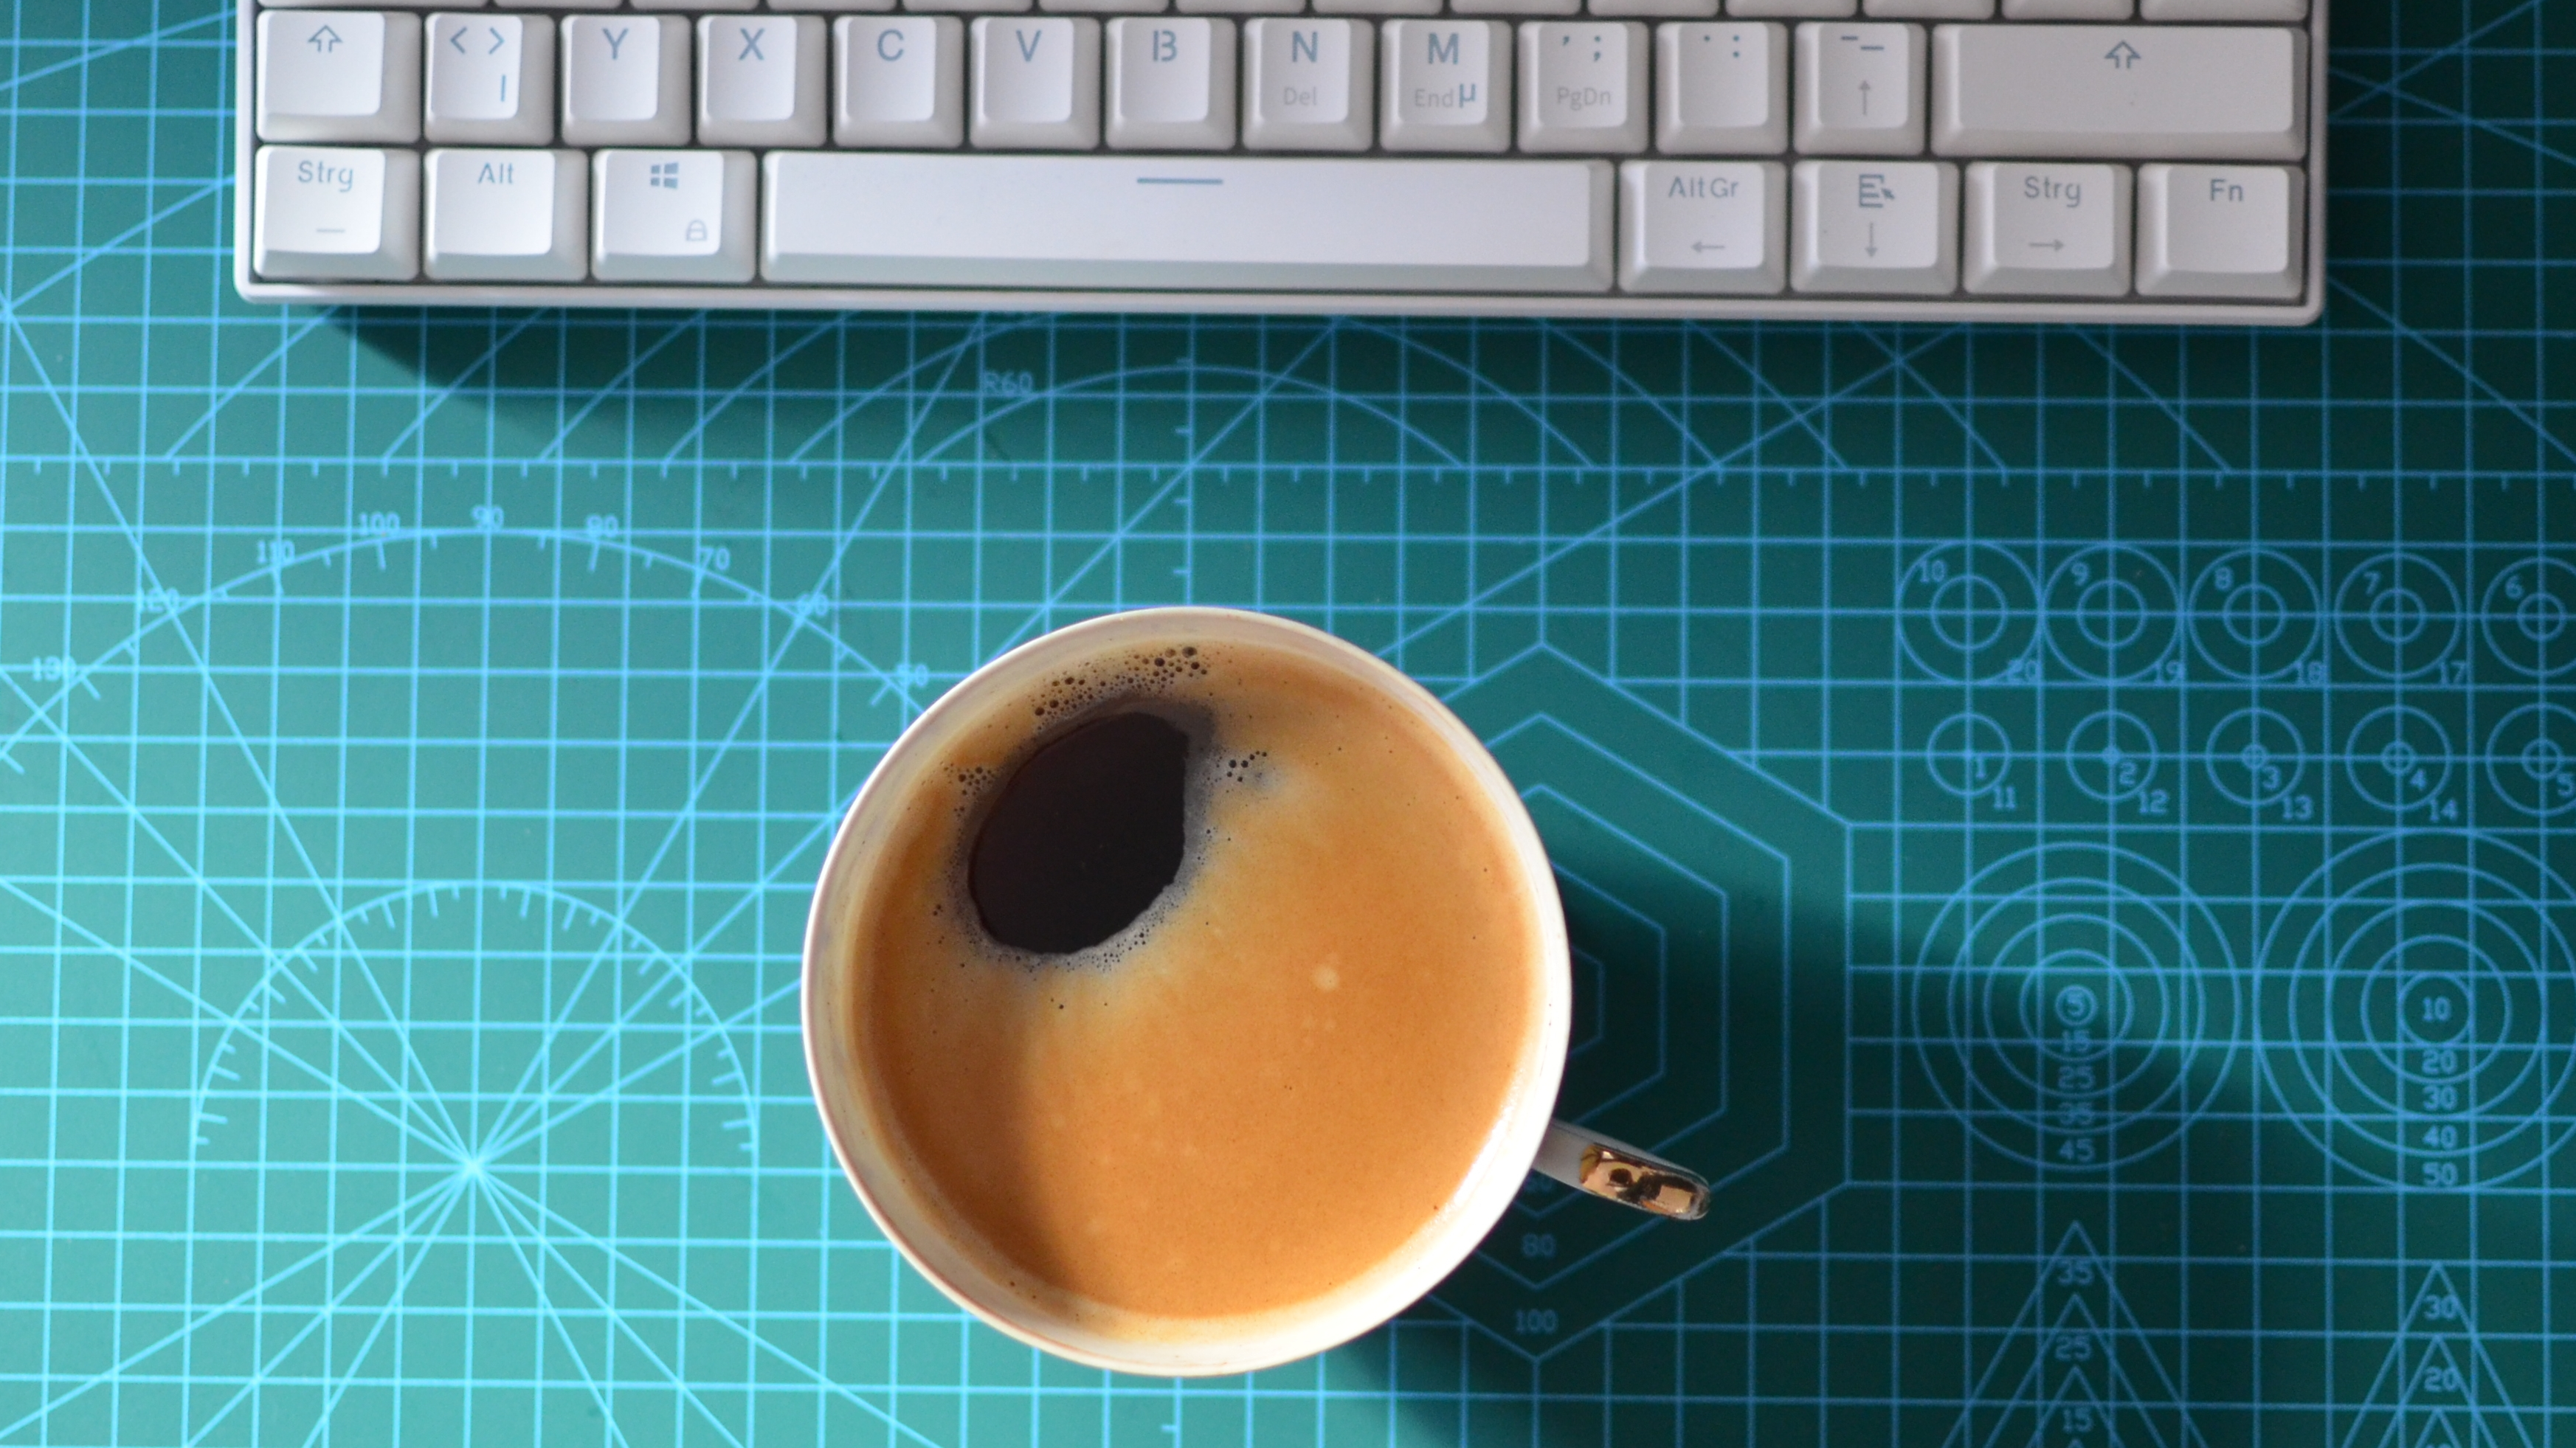
\includegraphics[width=\paperwidth]{./img/coffee.JPG}}
\begin{frame}[plain,b]
\centering
\LARGE Thanks for joining in the morning!\vspace{4ex}
\end{frame}
}%<---- Finish local changes

\begin{frame}[label={sec:orgb62bcd2}]{Presentation outline}
\tableofcontents
\end{frame}

\section{{\bfseries\sffamily TODO} Aligning BDDs}
\label{sec:orgb902488}
\subsection{On BDD representations}
\label{sec:org2db8d43}
\begin{frame}[label={sec:org6053e5a}]{What is an (O)BDD?}
\begin{columns}
\begin{column}[t]{0.40\columnwidth}
\textbf{In a nutshell:}
\begin{itemize}
\item A (maybe weighted) layered (D)AG
\item Two outgoing arcs from each node
\item One root, two terminals\vspace{2ex}

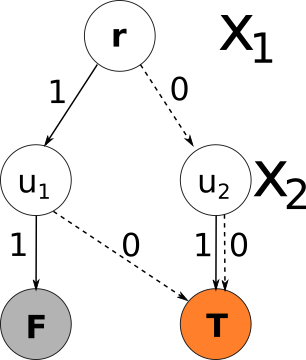
\includegraphics[width=0.6\textwidth]{./img/simple-BDD.png}
\end{itemize}
\end{column}
\begin{column}[t]{0.5\columnwidth}
\textbf{Applications:}
\begin{itemize}
\item Can encode a Boolean function \ldots{}
\item \ldots{} or a combinatorial opt problem.
\end{itemize}

\textbf{How it works:}
\begin{itemize}
\item A layer corresponds to a ``decision'' (binary variable),
\item \alert{one-arc} (or yes-arc) -- \(x_i=1\),
\item \alert{zero-arc} (or no-arc) -- \(x_i=0\).
\item A \alert{path} from root to terminal corresponds to an assignment of all
variables.
\end{itemize}
\end{column}
\end{columns}
\end{frame}
\begin{frame}[label={sec:org1601c04}]{Order of variables matters: a MIS example}
\begin{columns}
\begin{column}{0.2\columnwidth}
\centering
\textbf{Original graph:}\vspace{2ex}
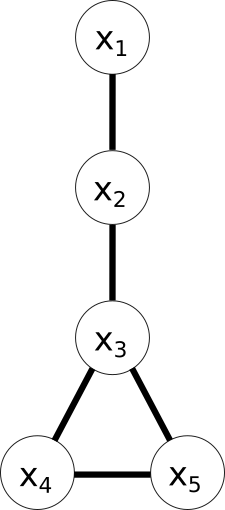
\includegraphics[height=0.6\textheight]{./img/BDDsampleGraph.png}
\end{column}
\begin{column}{0.35\columnwidth}
\centering
\textbf{14 nodes:}\vspace{2ex}
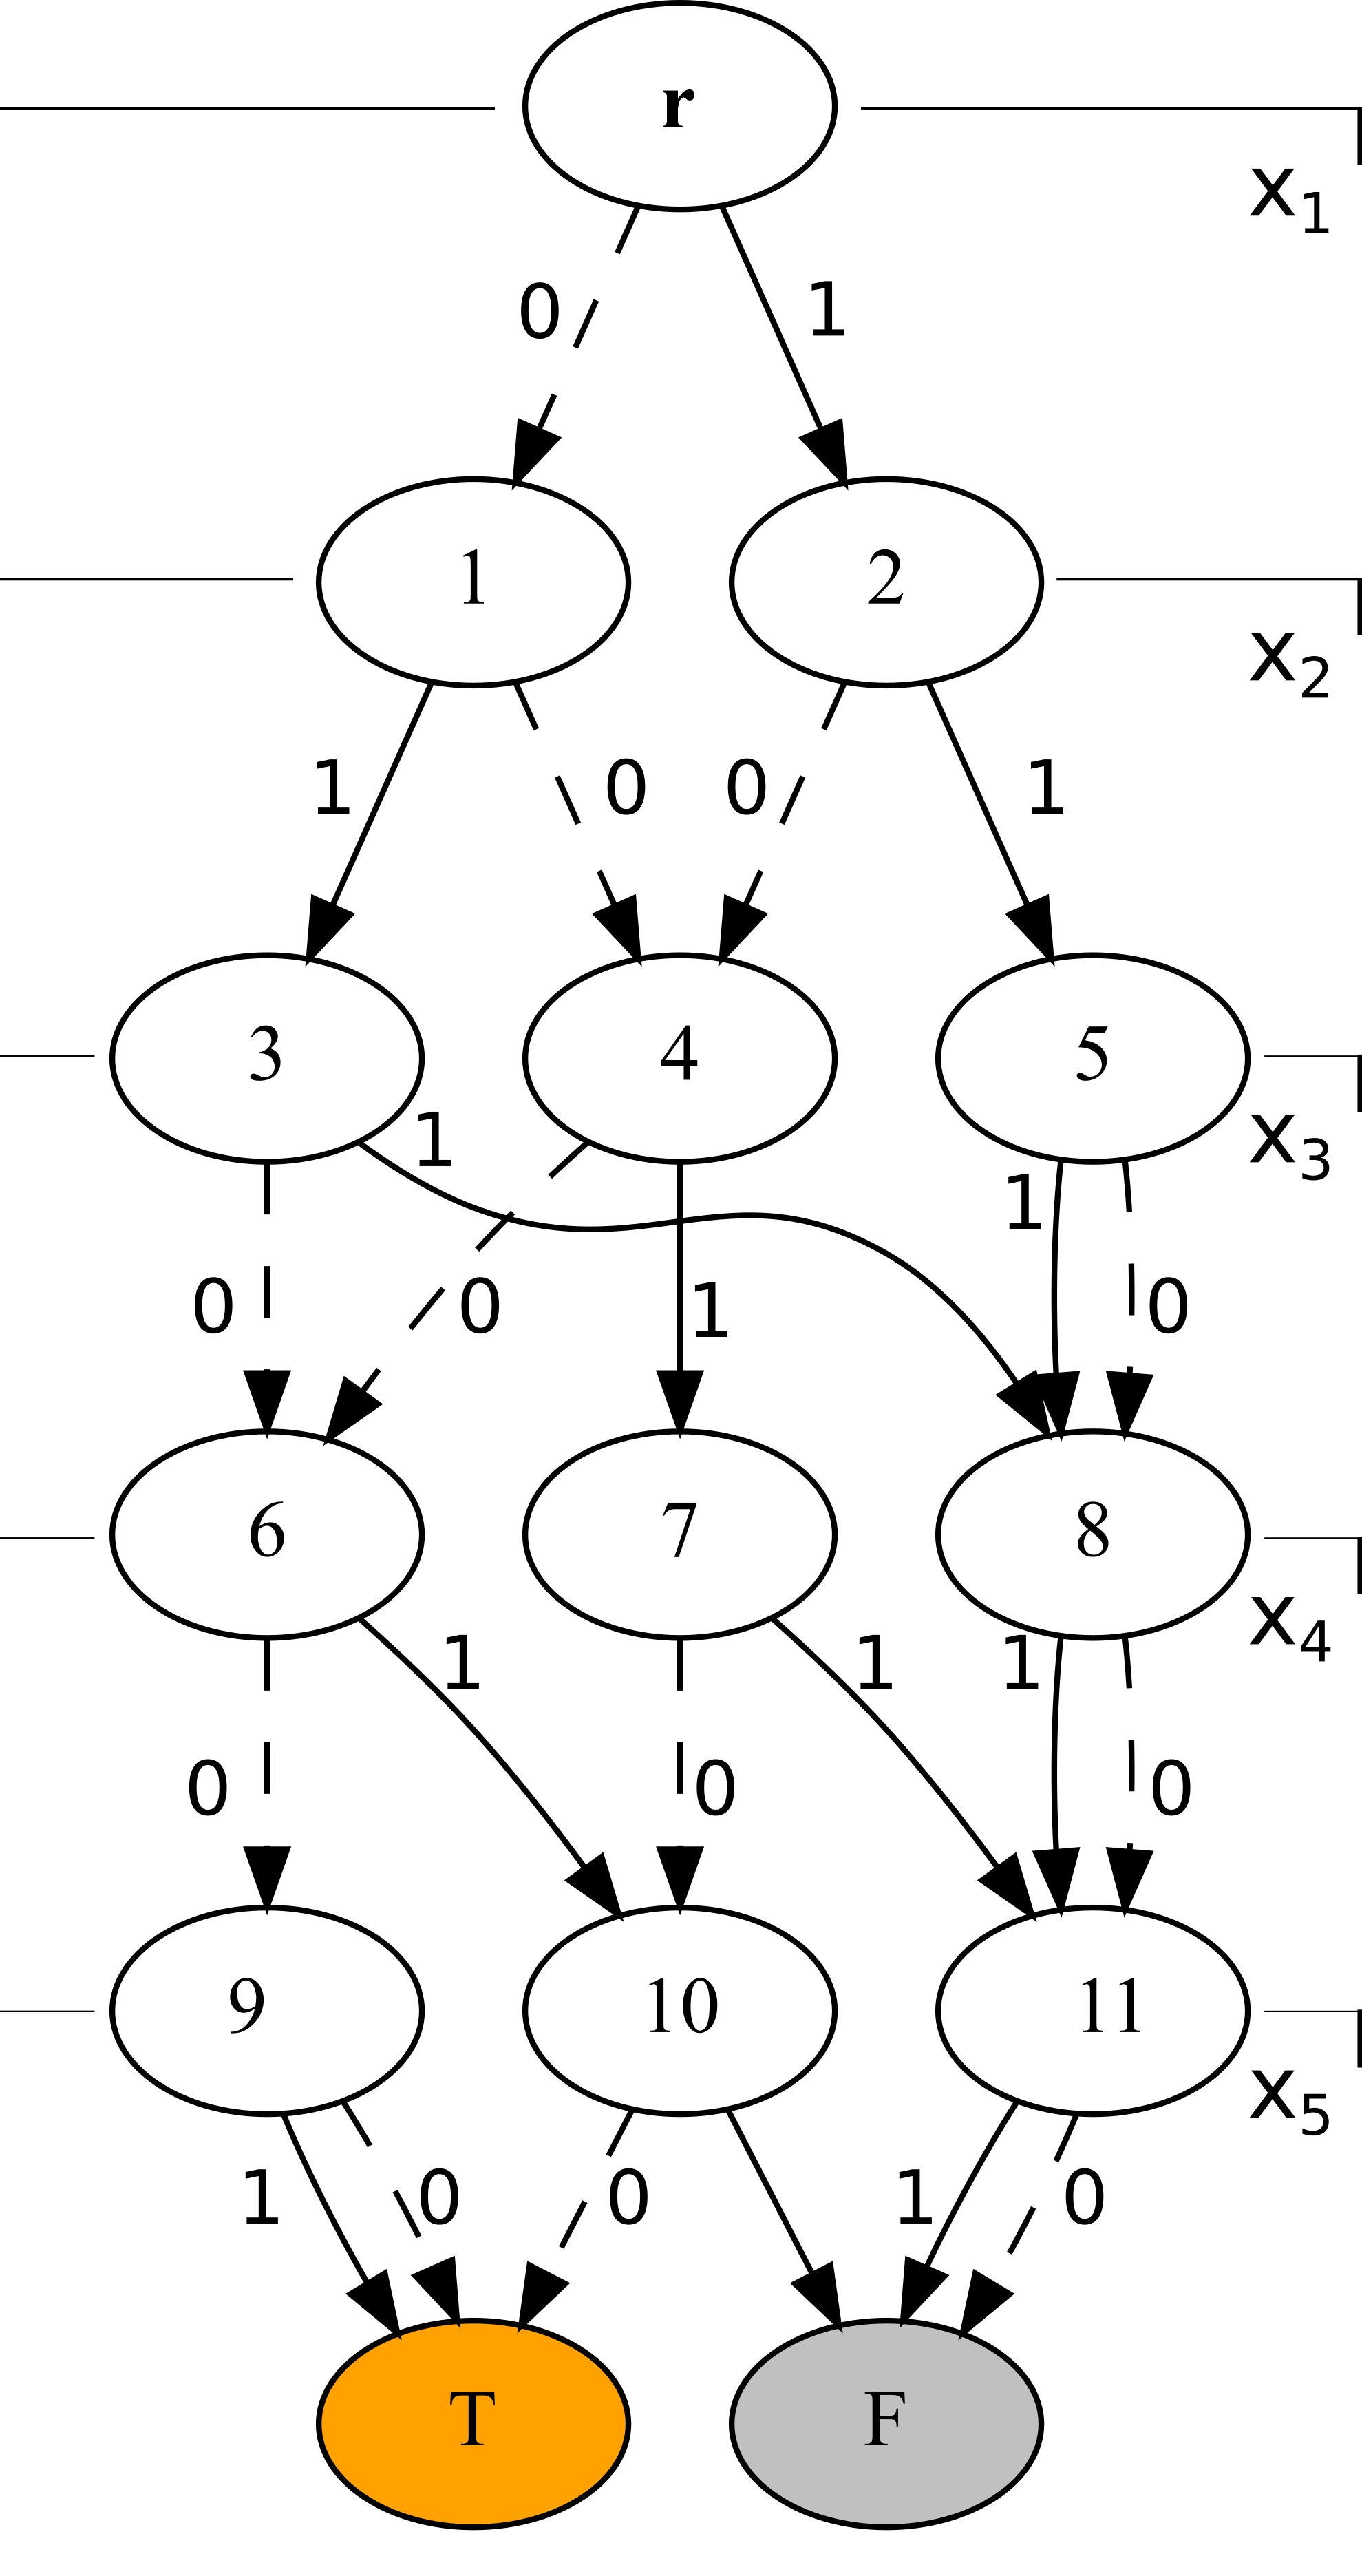
\includegraphics[height=0.7\textheight]{./img/BDDsampleRep1.png}
\end{column}
\begin{column}{0.55\columnwidth}
\centering
\textbf{17 nodes:}\vspace{2ex}
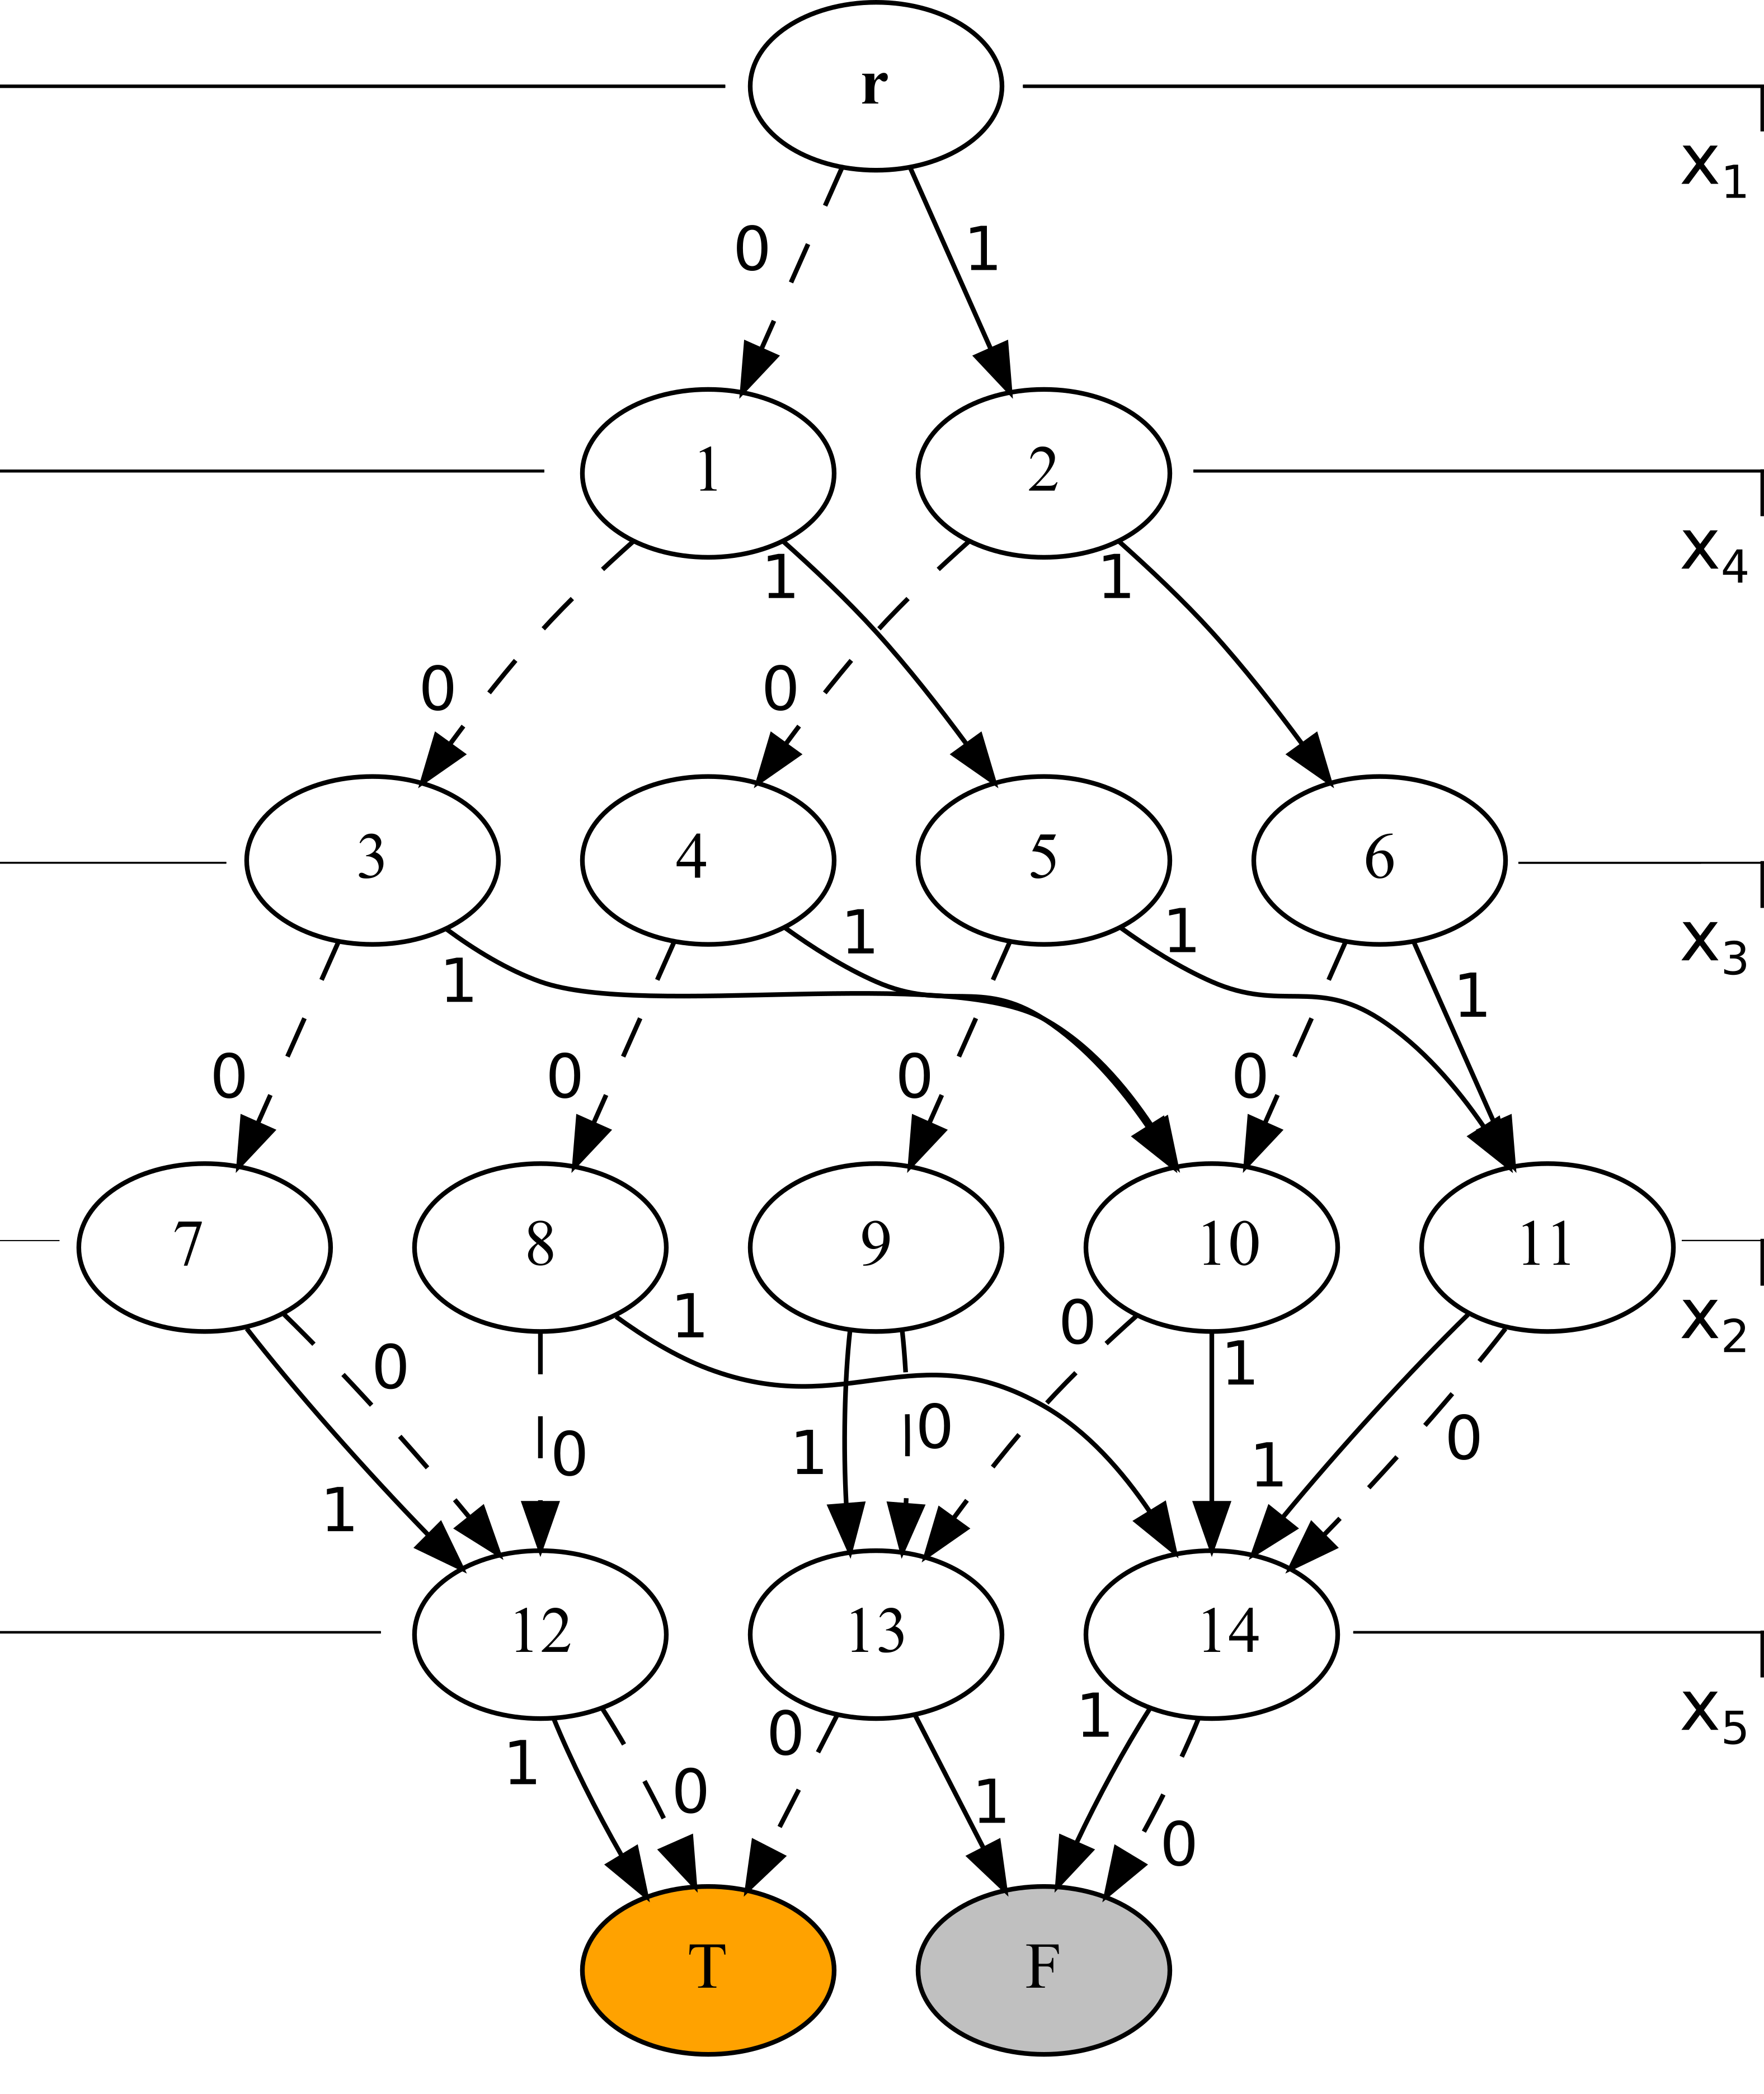
\includegraphics[height=0.7\textheight]{./img/BDDsampleRep2.png}
\end{column}
\end{columns}
\end{frame}
\begin{frame}[label={sec:org1898885}]{The \alert{same} order of variables also matters}
\begin{itemize}
\item Many problems can be reformulated as a set of (connected) instances
over a collection of BDDs.
\item If we have the same order of variables: \cite{lozano2020} proposed an algorithm
how to tackle such instances.
\item So, finding a good shared order of variables might be desirable.
\end{itemize}
\end{frame}
\begin{frame}[label={sec:org4d7d61c}]{A motivating example: t-UFLP}
\begin{columns}
\begin{column}{0.2\columnwidth}
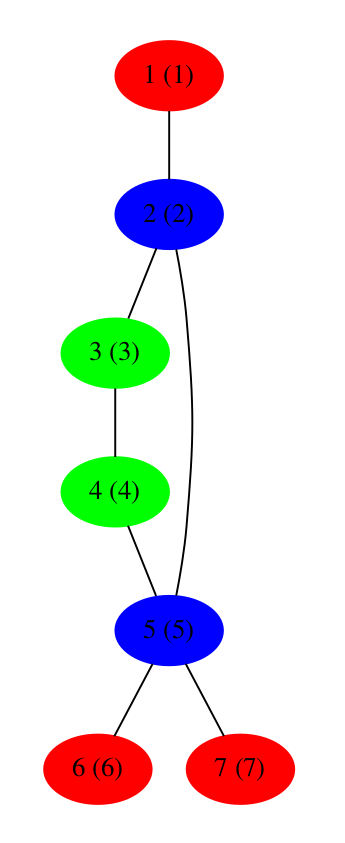
\includegraphics[height=0.8\textheight]{./img/tUFLP.png}
\end{column}
\begin{column}{0.8\columnwidth}
\textbf{Assume:}
\begin{itemize}
\item A graph; can \alert{locate} a facility at any point,
\item A located facility \alert{covers} all neighboring points.
\end{itemize}

\textbf{Objective:} cover all points at min cost.

\textbf{Constraints:}
\begin{itemize}
\item Each point implies a facility \alert{``type''},
\item There is a limit on number of facilities by type.
\end{itemize}
\end{column}
\end{columns}
\end{frame}
\begin{frame}[label={sec:org2eb9891}]{How to merge two diagrams?}
\centering
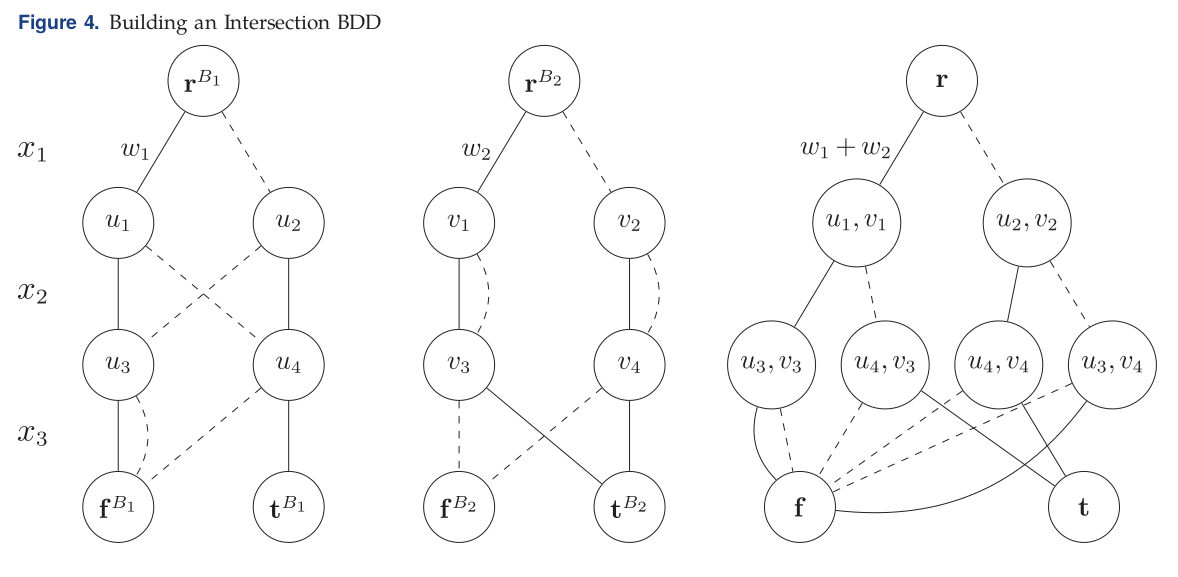
\includegraphics[width=\textwidth]{./img/merging.png}

Source: \cite{lozano2020}
\end{frame}
\begin{frame}[label={sec:org6d0673a}]{A motivating example: t-UFLP}
\begin{columns}
\begin{column}{0.2\columnwidth}
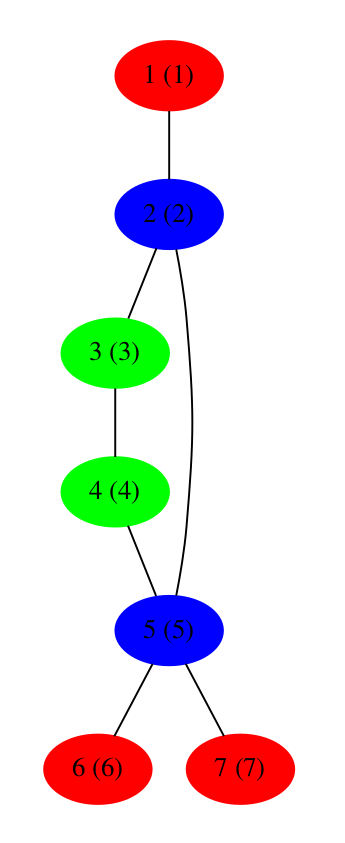
\includegraphics[height=0.8\textheight]{./img/tUFLP.png}
\end{column}
\begin{column}{0.8\columnwidth}
\textbf{Plan of attack:}
\begin{itemize}
\item Formulate the problem with two BDDs,
\item \tikzmarkin<2->{this}Enforce the shared order of variables\tikzmarkend{this}, \onslide<2->{\alert{$\leftarrow$ this part}}
\item Merge (``intersect'') the two diagrams into one*
\item Solve a shortest-path in the intersection DD.
\end{itemize}
\end{column}
\end{columns}
\end{frame}
\begin{frame}[label={sec:orgcc66cfb}]{In this section:}
\begin{itemize}
\item BDD alignment problem,
\item A simplified model / heuristic,
\item Numerical experiments on aligning BDDs.
\end{itemize}
\end{frame}
\subsection{BDD alignment (``original'') problem}
\label{sec:orgcf1ab80}
\begin{frame}[label={sec:org39e79f7}]{BDD alignment problem}
Let us denote \(T^*[D,\vec{v}]\) -- a ``transformed'' version of BDD \(D\) to variable order \(\vec{v}=(v_1,\ldots,v_N)\). Then:
\begin{block}{BDD Alignment Problem / ``original'' problem}
\begin{align*}
     s^* = \min_{\vec{v}} \Big\{ |T^*[A, \vec{v}]| + |T^*[B, \vec{v}]| \Big\},
\end{align*}
\end{block}
where \(|D|\) is the number of nodes in diagram \(D\). The problem is NP-hard (because the min single BDD is NP-hard).
\end{frame}
\begin{frame}[label={sec:orgb5f21dd}]{Research context}
\begin{itemize}
\item Vast literature on minimizing single BDD.
\item One of the central ideas: ``Dynamic variable reordering'' / \alert{Sifting} algorithm (we will use it as a baseline).
\item Limited consideration of the multi-BDD version, and all working with BDDs (obviously).
\end{itemize}
\begin{block}{The purpose of this work}
Try to avoid manipulations with BDD as much as possible, by introducing a
``simpler'' auxiliary problem.
\end{block}
\end{frame}
\subsection{The simplified problem}
\label{sec:org8e8be28}
\begin{frame}[label={sec:org0bdb032}]{How the BDDs are transformed?}
\end{frame}
\begin{frame}[label={sec:org2822e2c}]{The simplified problem}
\end{frame}
\begin{frame}[label={sec:orgf09fe1d}]{Plan of attack with the simplified problem}
\end{frame}
\begin{frame}[label={sec:org8d50c31}]{How to solve it now? Key properties}
\end{frame}
\begin{frame}[label={sec:org467ae60}]{Branch\ldots{}}
\end{frame}
\begin{frame}[label={sec:org82dba8f}]{\ldots{} and bound.}
\end{frame}
\subsection{Numerical experiments}
\label{sec:org345e588}
\begin{frame}[label={sec:org9d133b2}]{Numerical experiments: strategy}
\begin{itemize}
\item First: consider the simplified problem in detail.
\item Then: solve the original problem, benchmark vs the baseline and consider scaling.
\item Analyze the solutions: original vs. simplified, problem structure.
\end{itemize}
\end{frame}

\begin{frame}[label={sec:org4cd5e49}]{Simplified problem: optima}
\begin{columns}
\begin{column}{0.5\columnwidth}
\centering
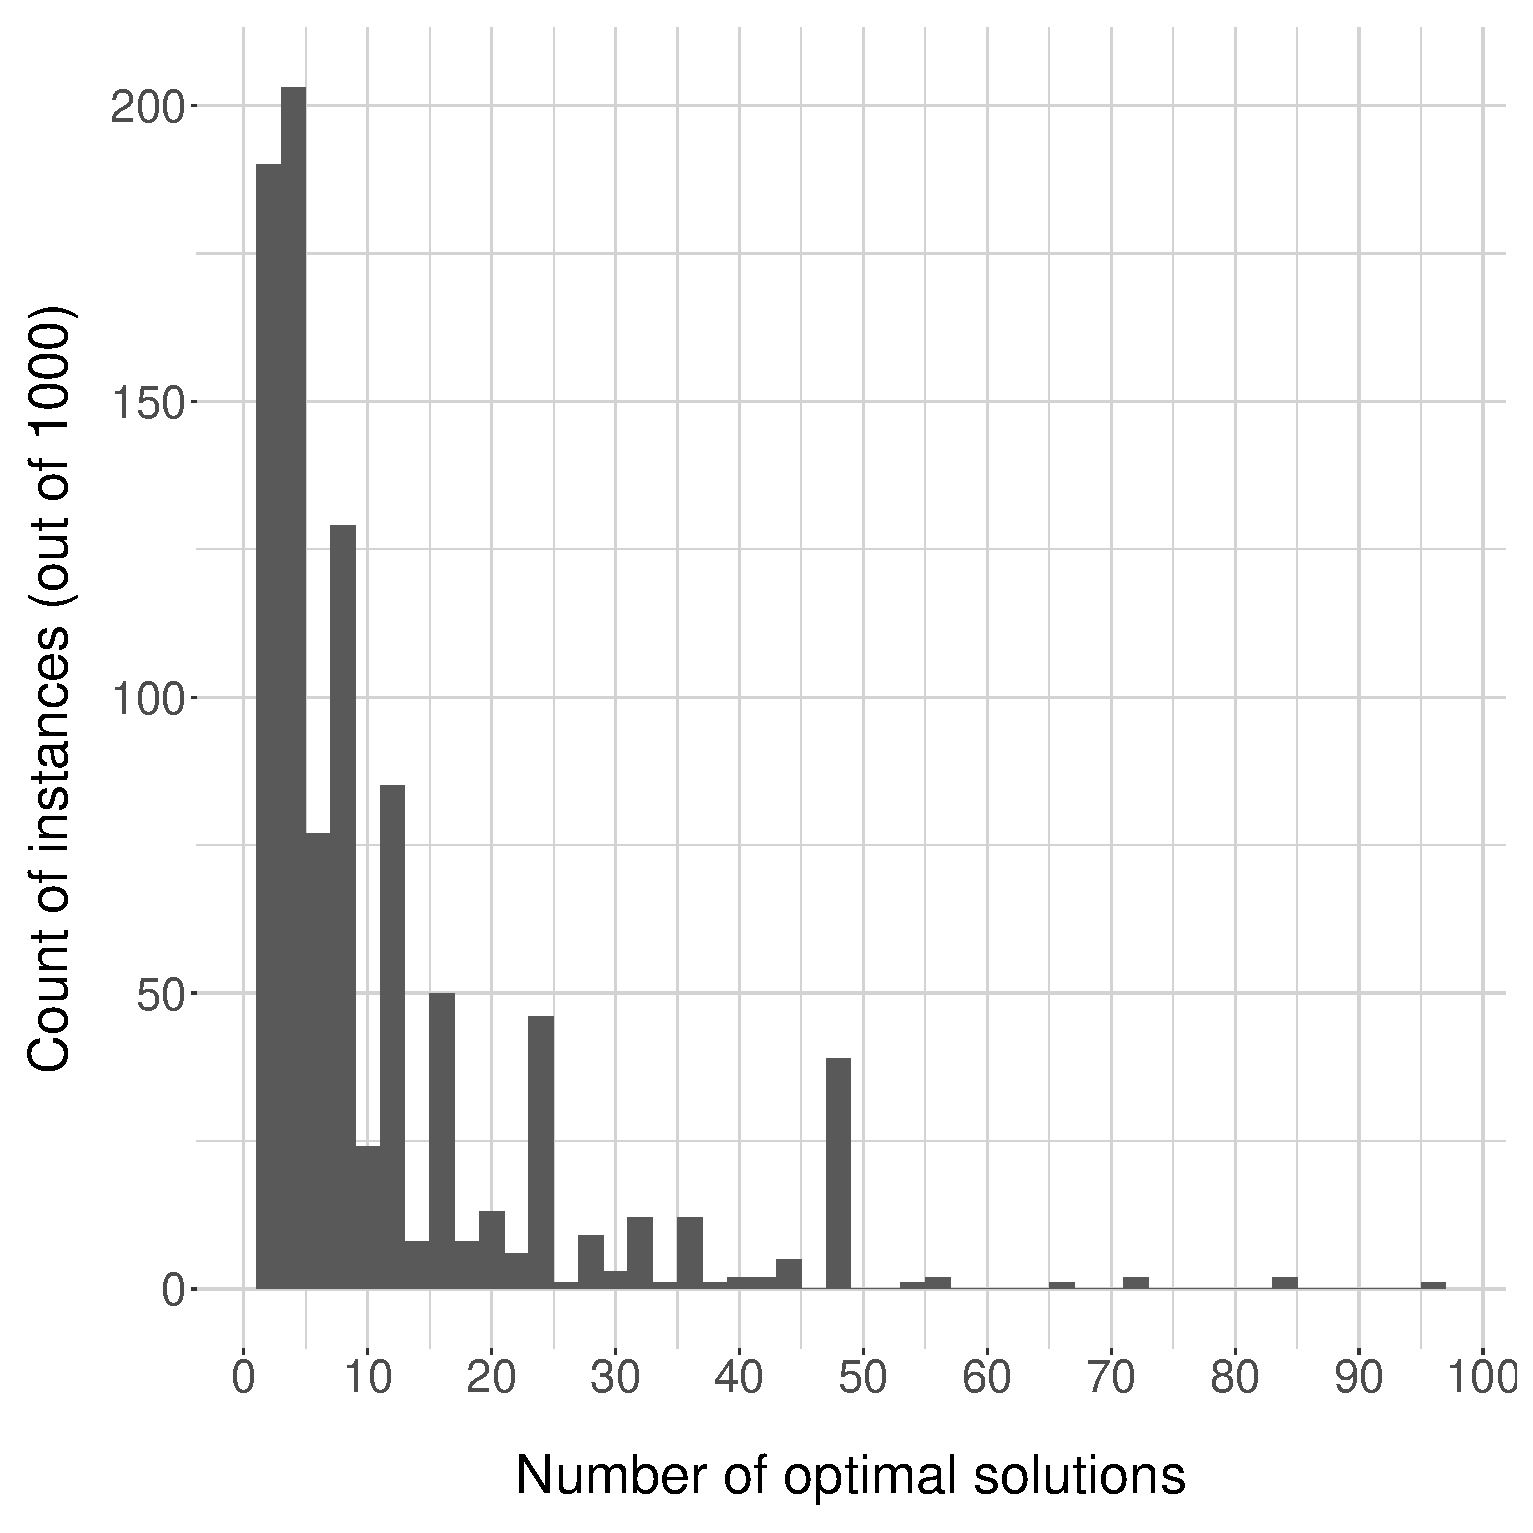
\includegraphics[width=\textwidth]{./img/no_opts.eps}
\end{column}
\begin{column}{0.5\columnwidth}
\centering
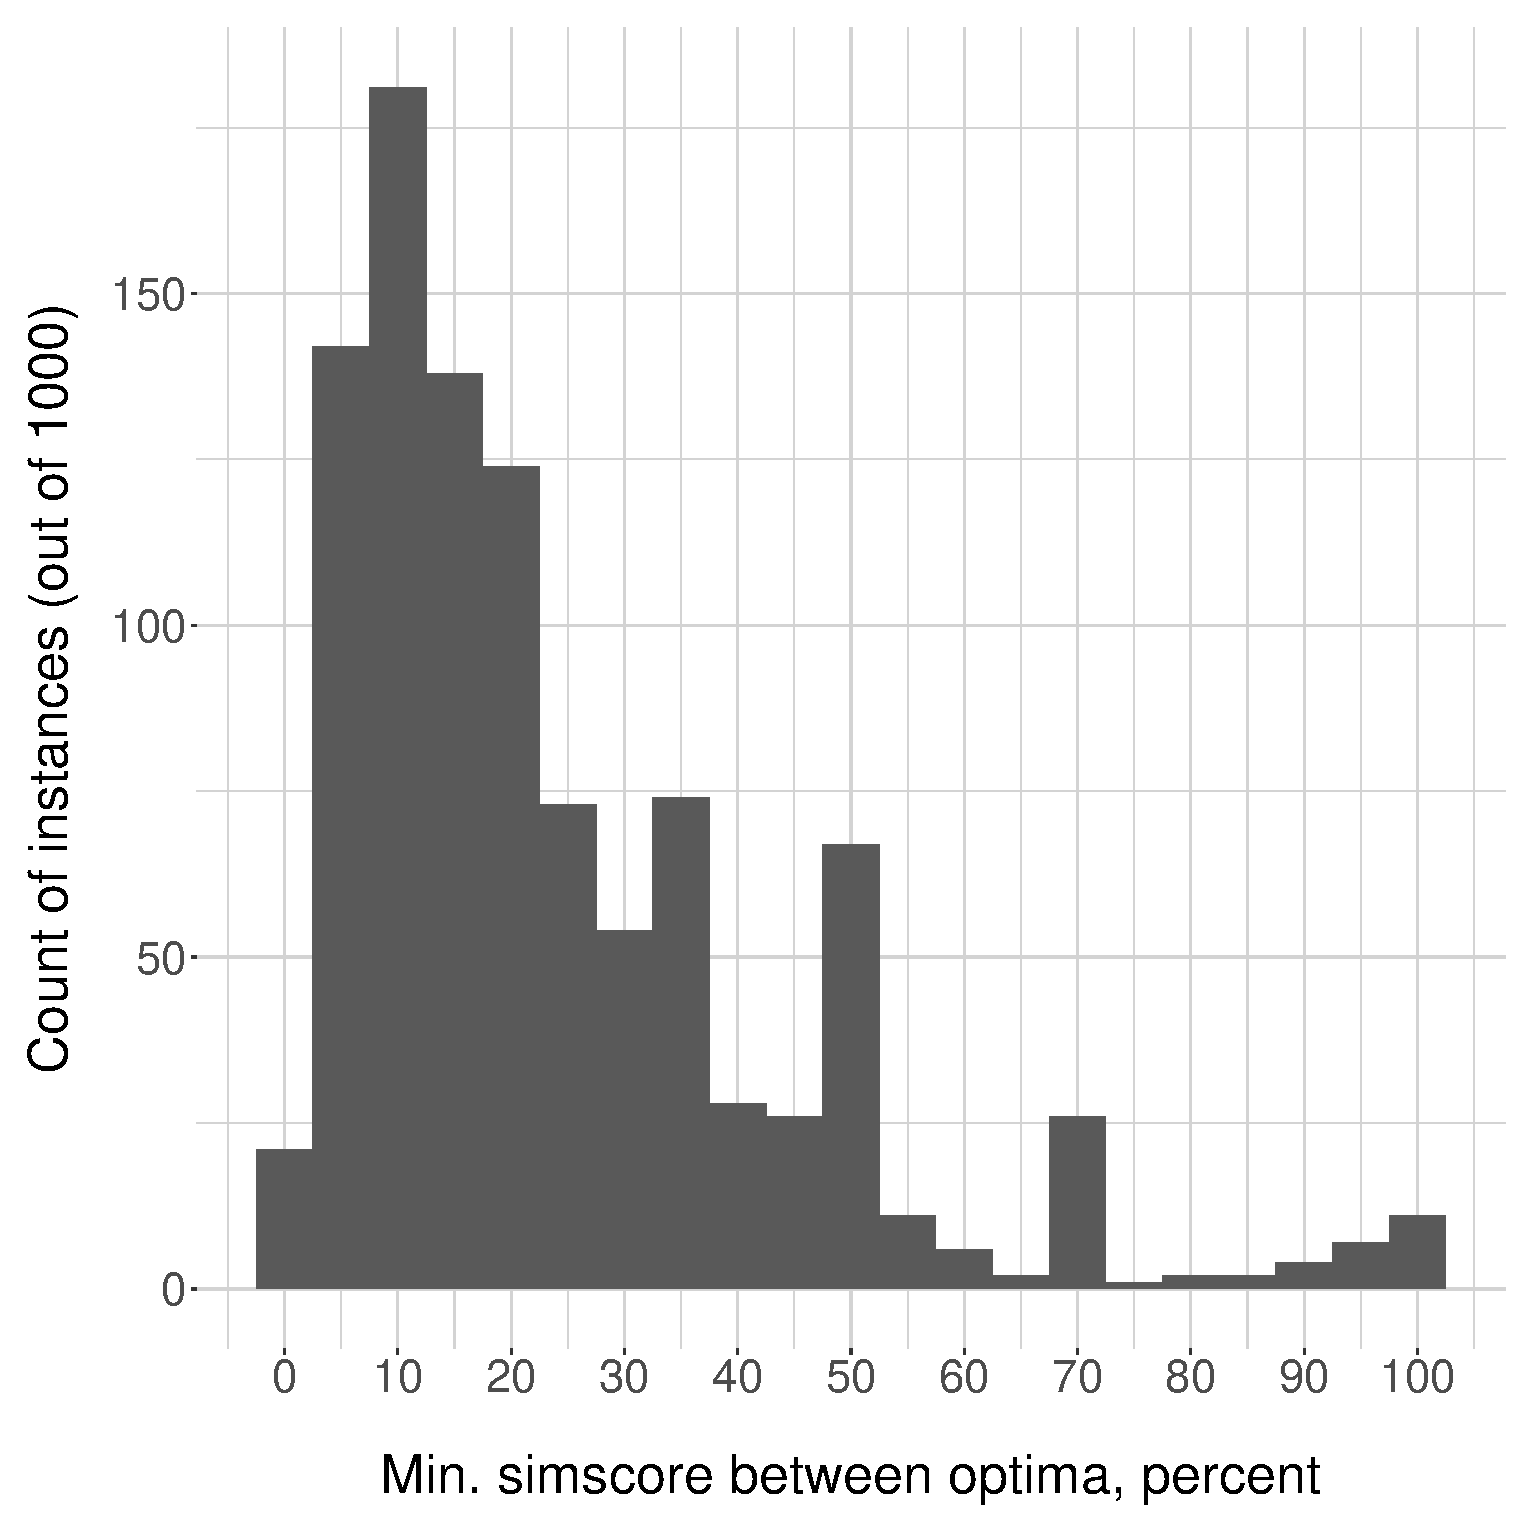
\includegraphics[width=\textwidth]{./img/opts_diam.eps}
\end{column}
\end{columns}
\end{frame}
\begin{frame}[label={sec:orgf8e88aa}]{Simplified problem: heuristics}
\centering
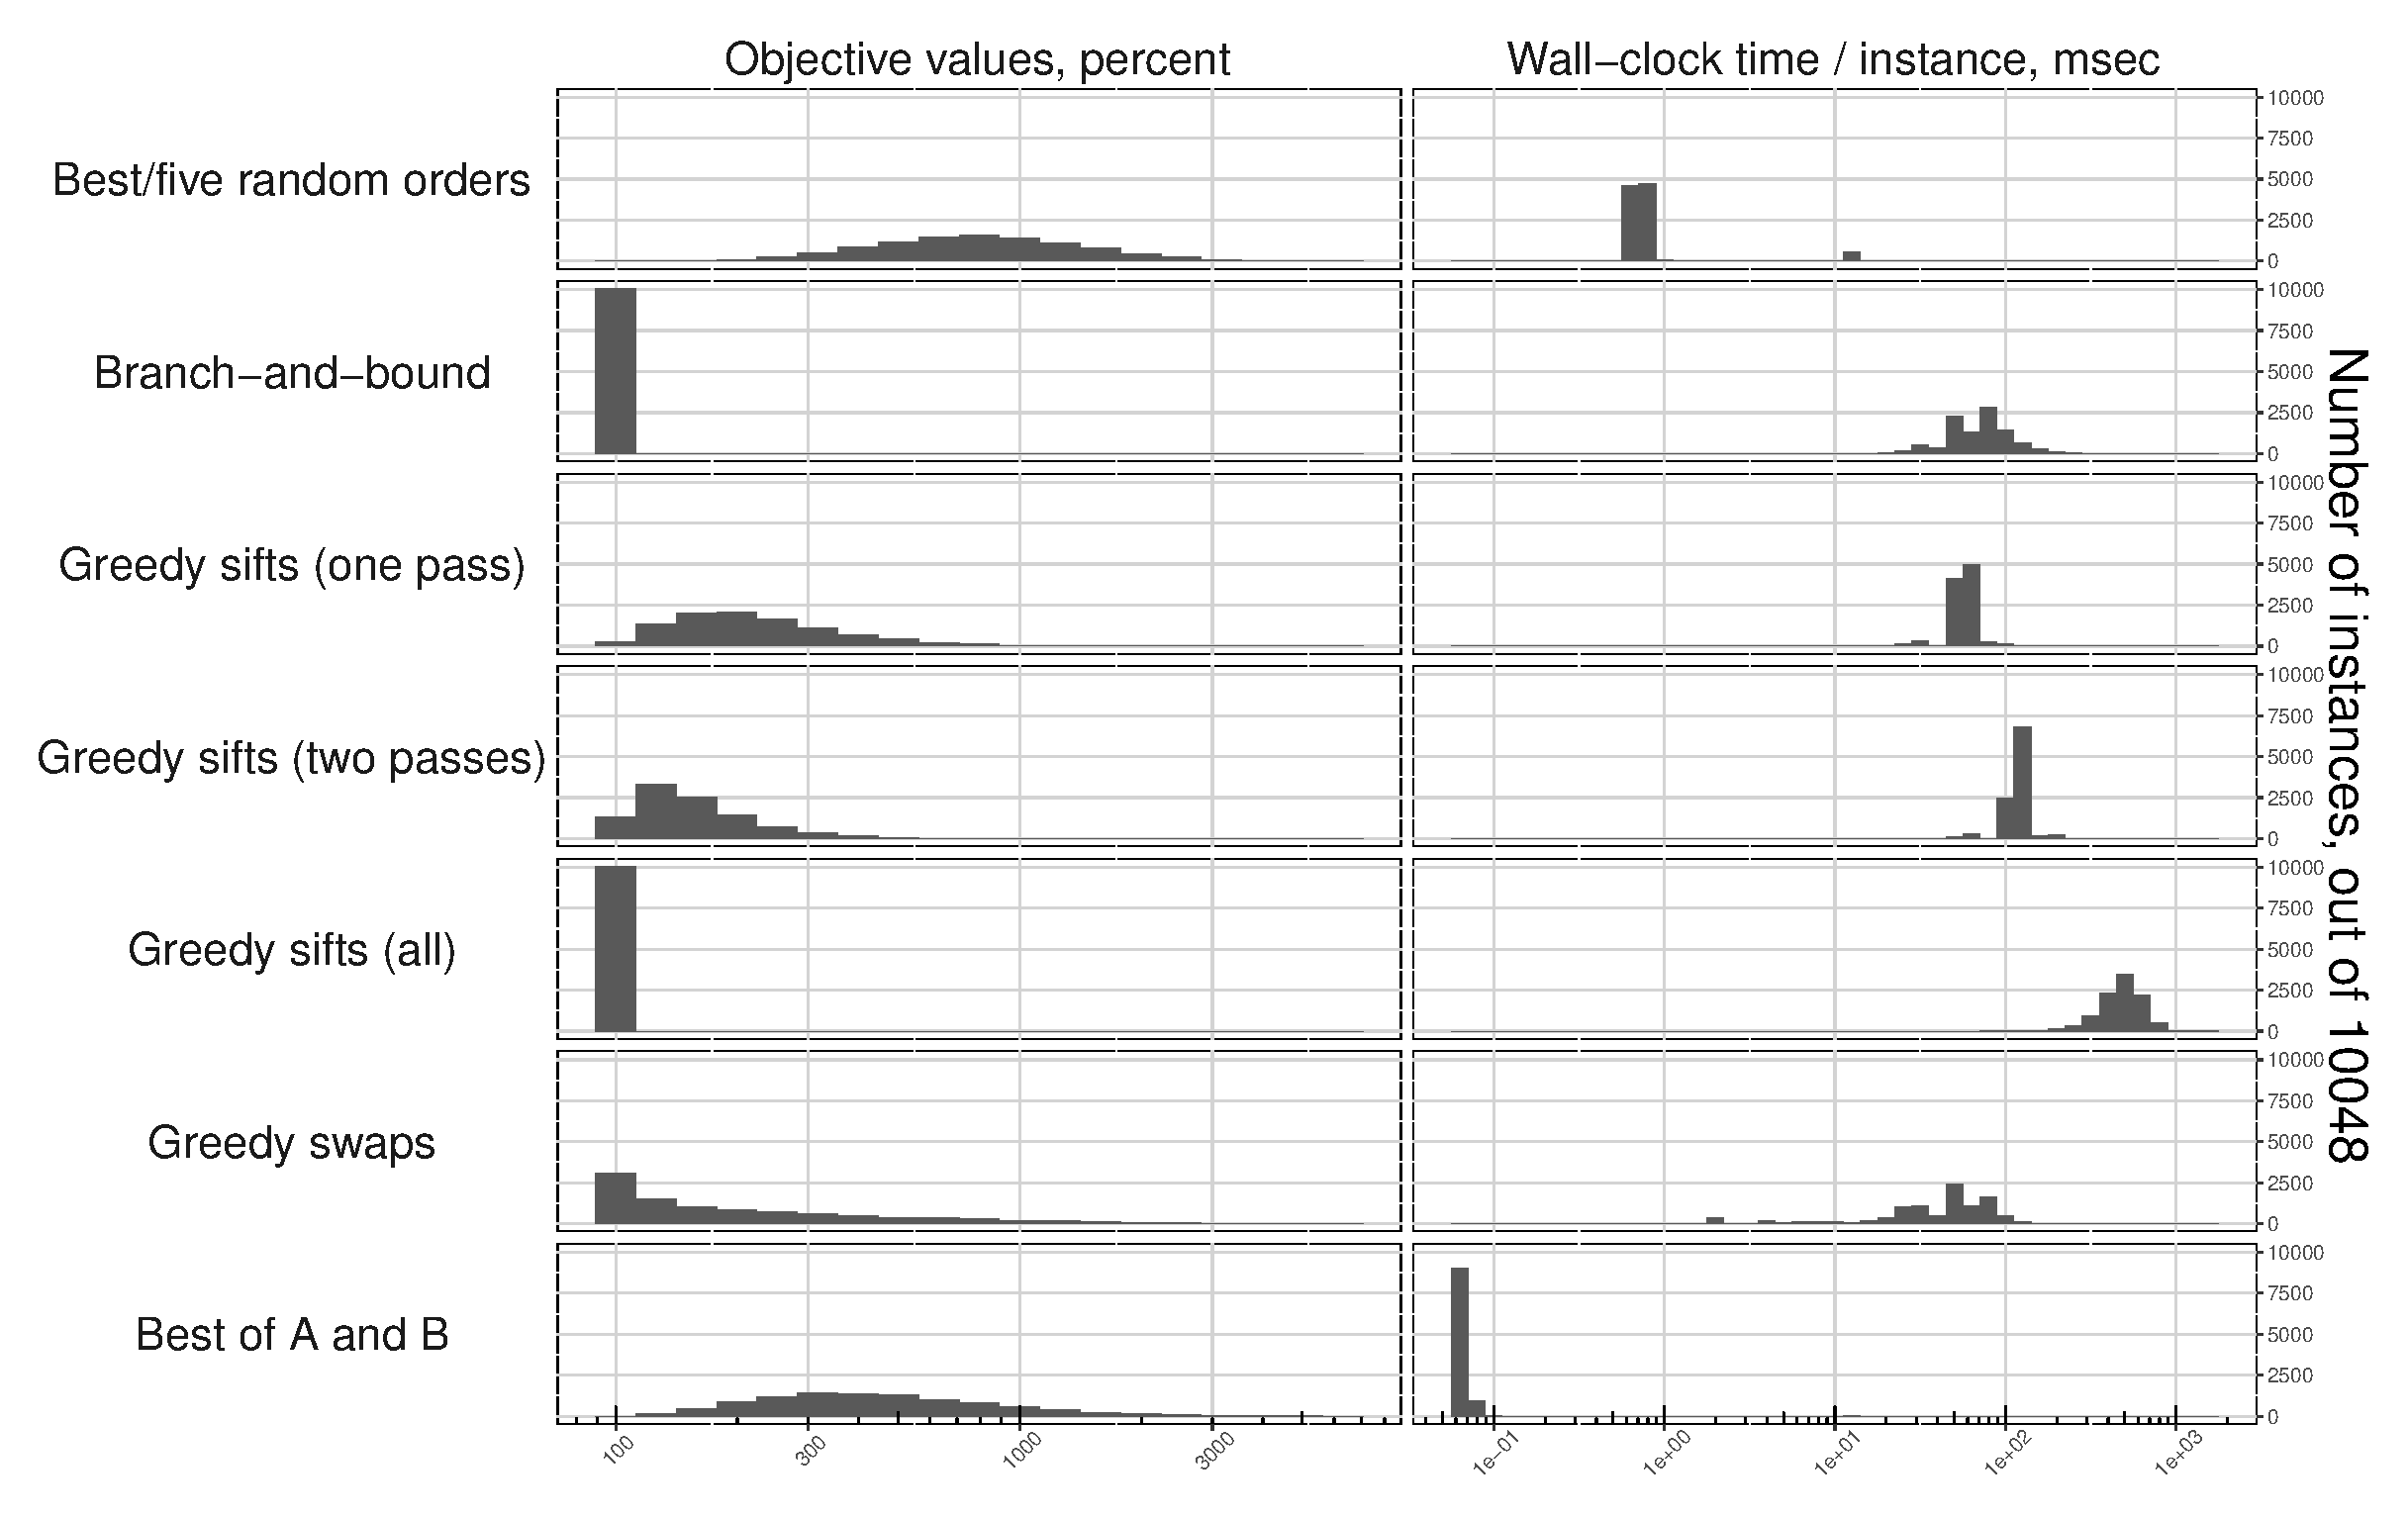
\includegraphics[width=\textwidth]{./img/simpl_heuristics.eps}
\end{frame}
\begin{frame}[label={sec:orgfe77061}]{Objectives relative to the ``greedy sifts''}
\centering
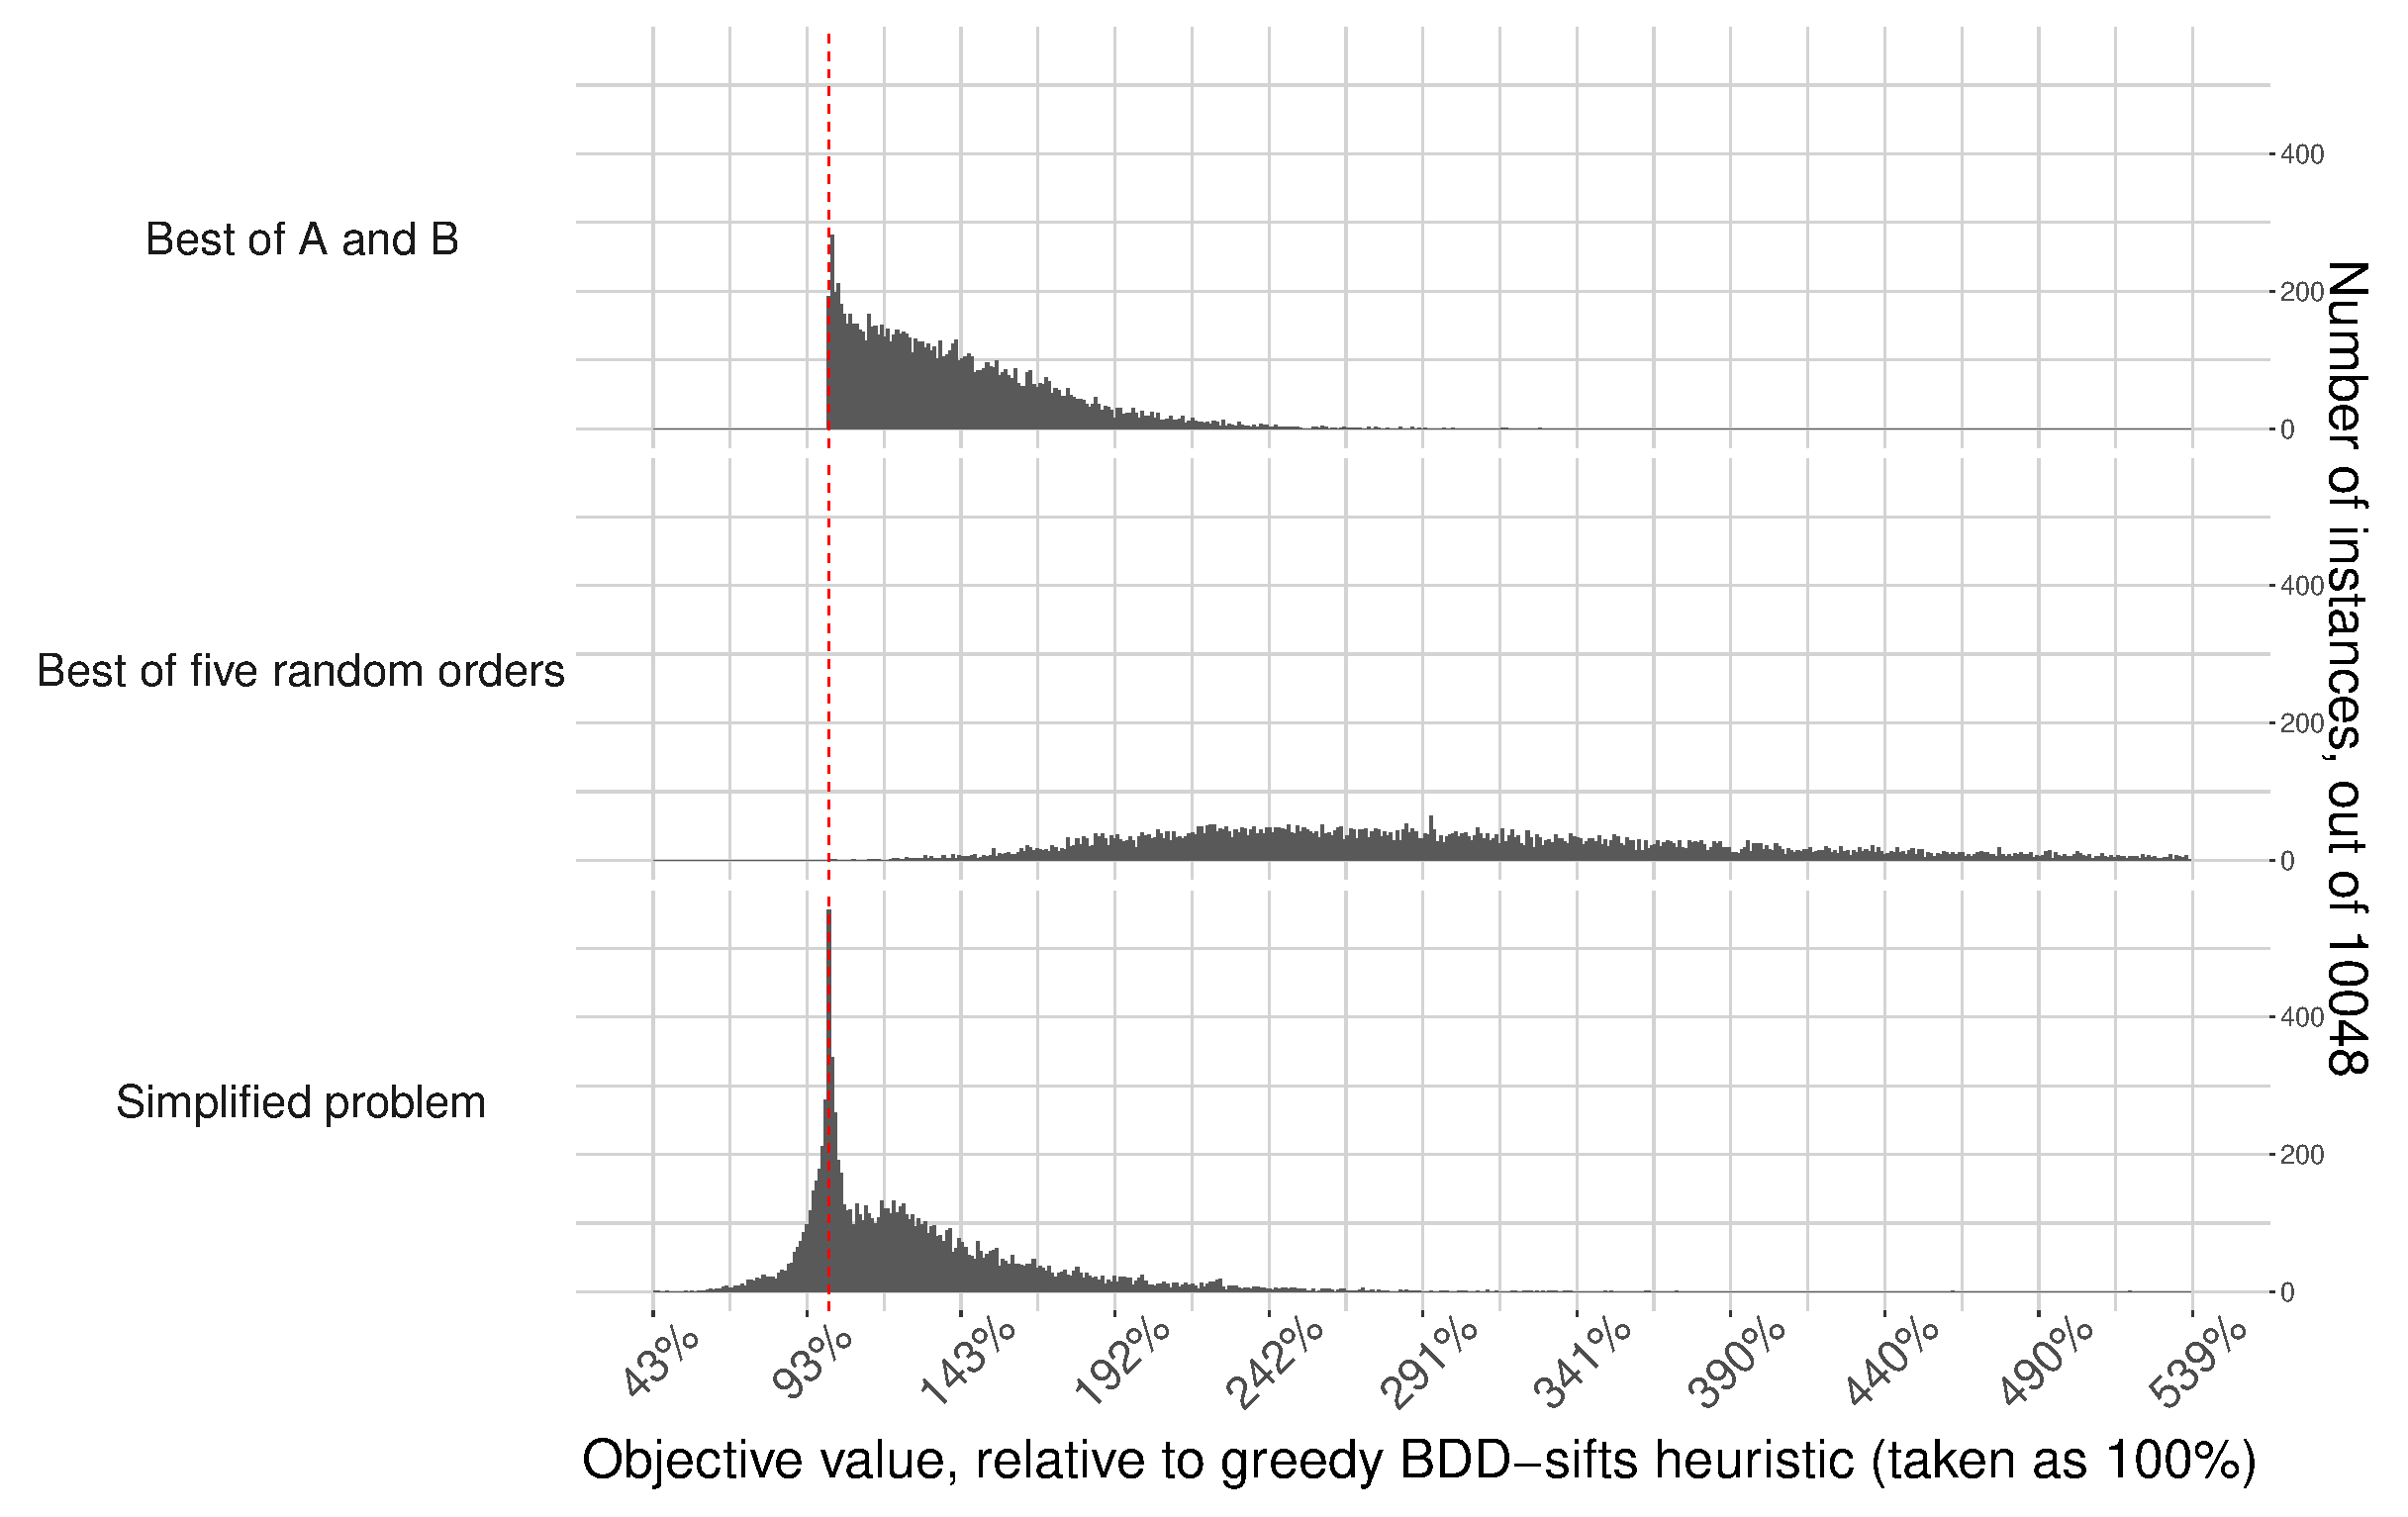
\includegraphics[width=\textwidth]{./img/orig_obj_histograms.eps}
\end{frame}
\begin{frame}[label={sec:org6158082}]{Scaling with the problem size}
\centering
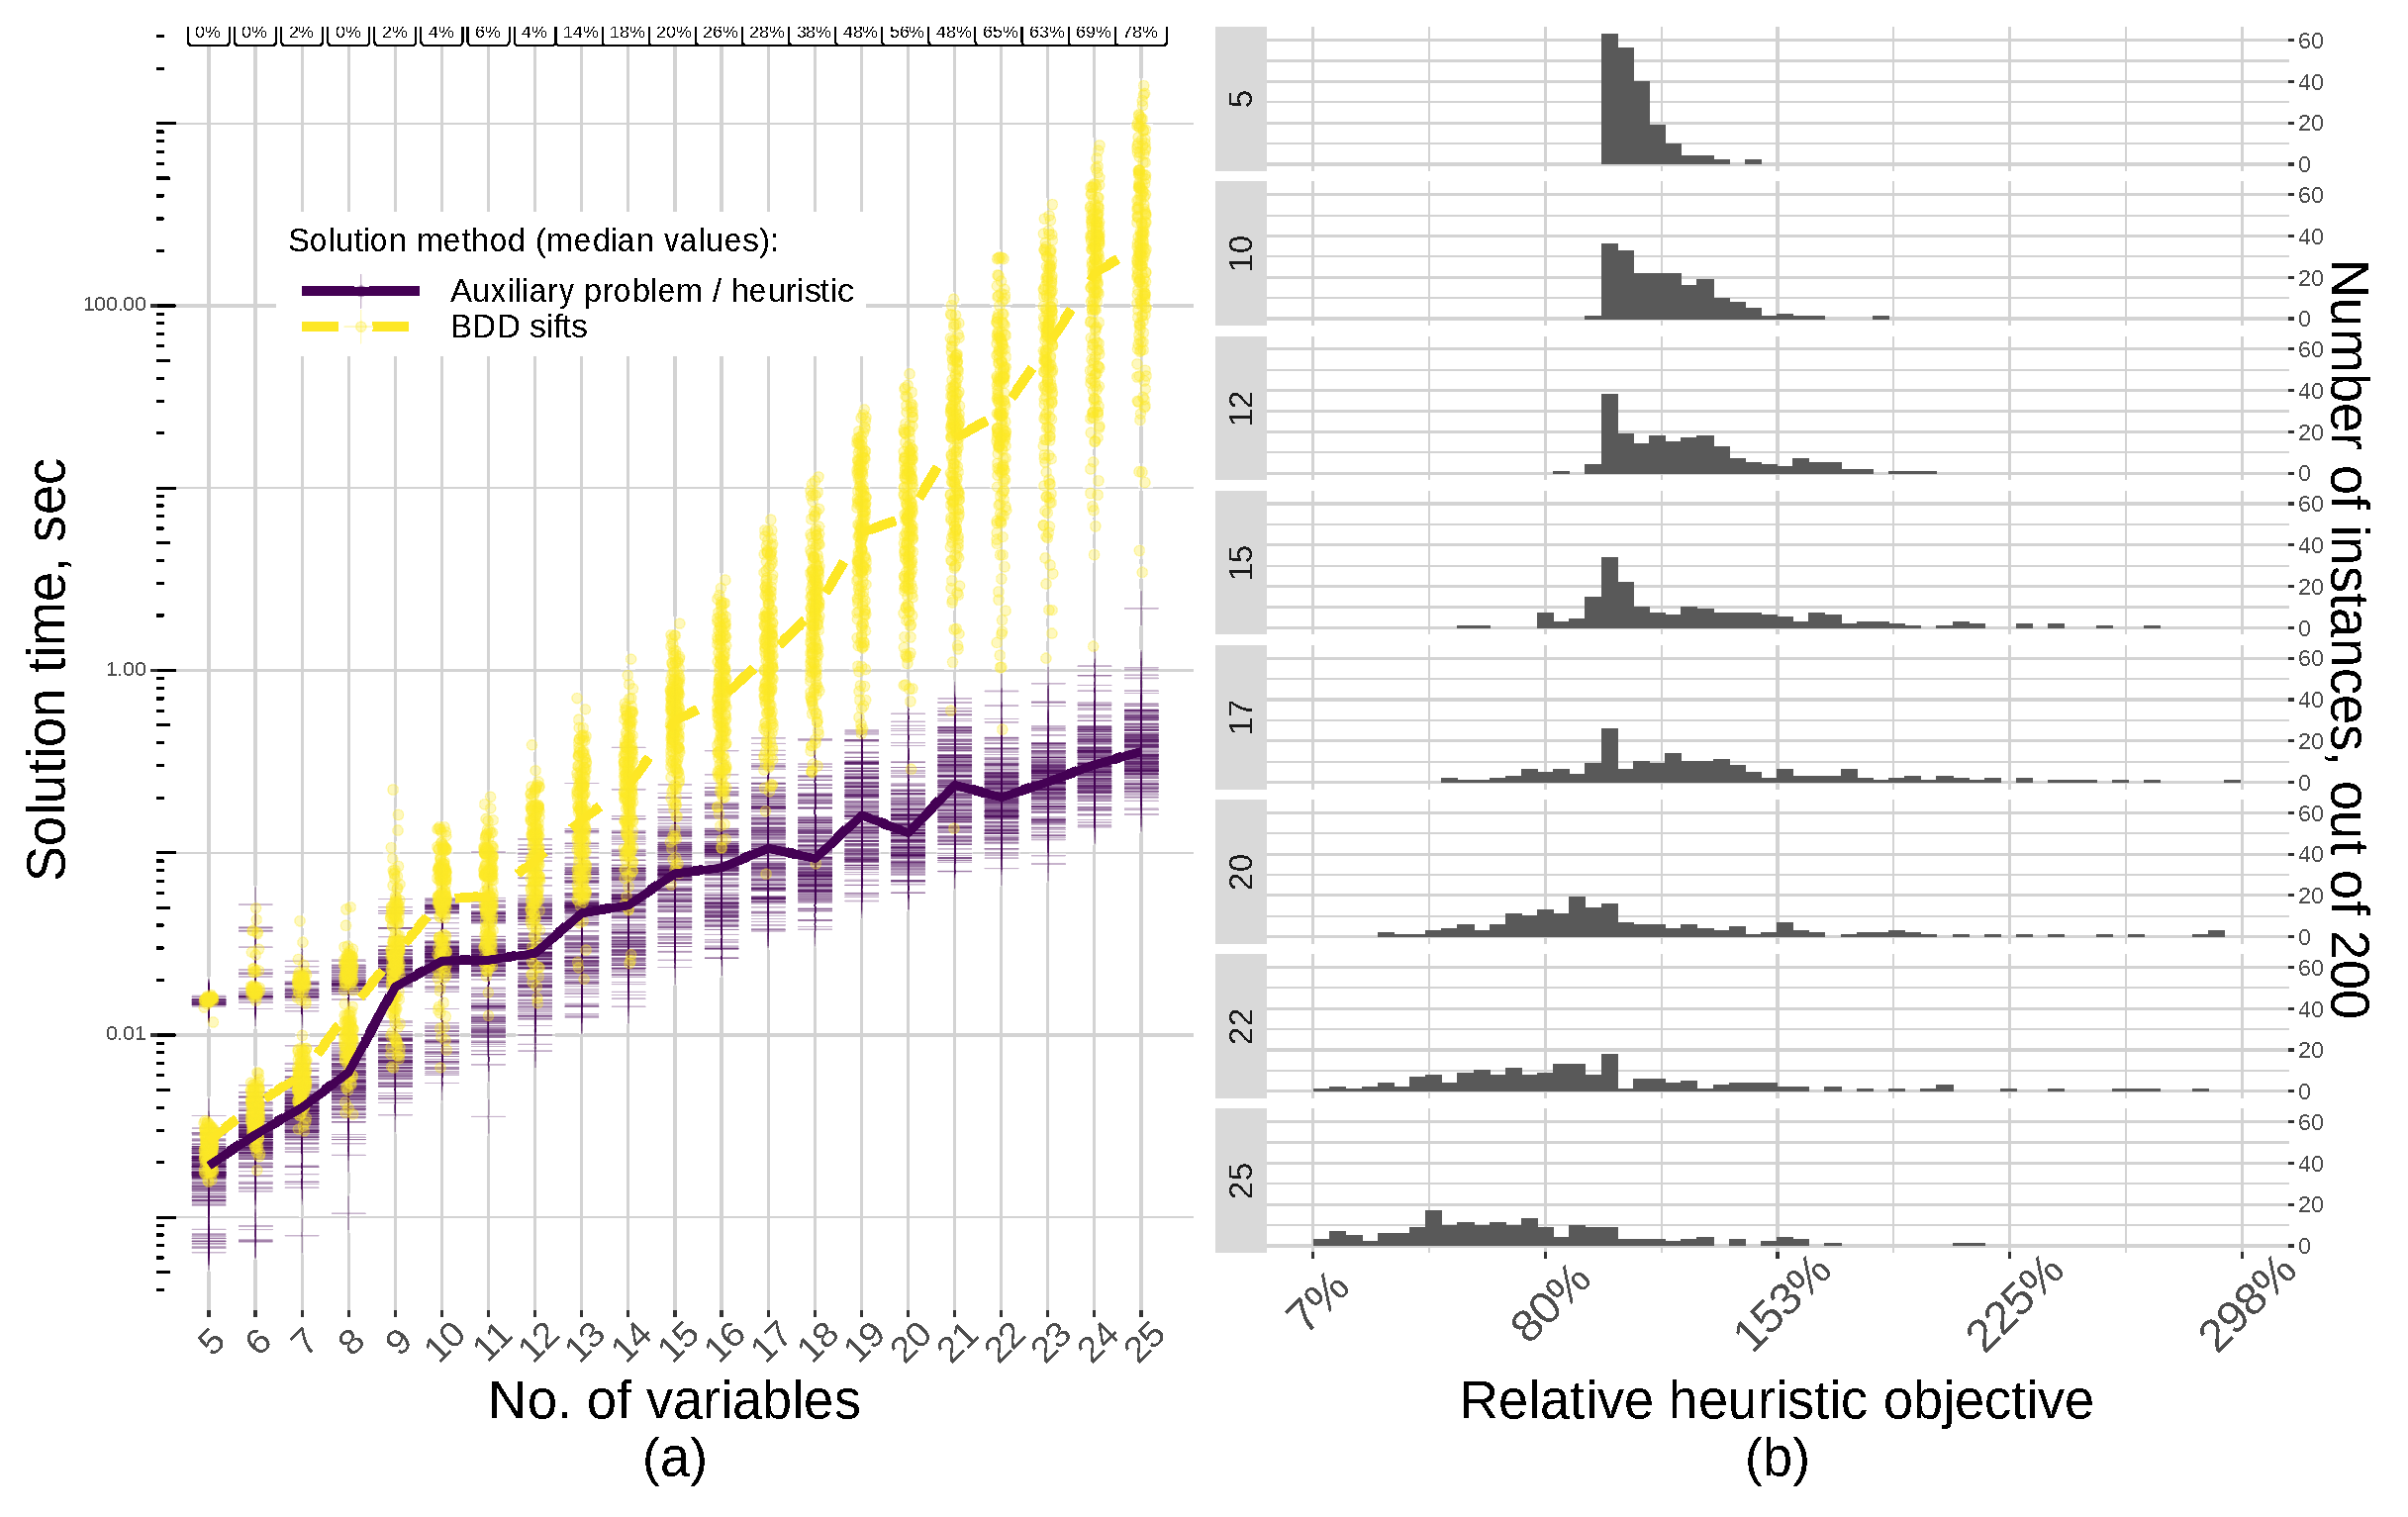
\includegraphics[width=\textwidth]{./img/orig_runtimes.eps}
\end{frame}

\begin{frame}[label={sec:org17b7fc5}]{Simplified vs. Original problem solutions}
\centering
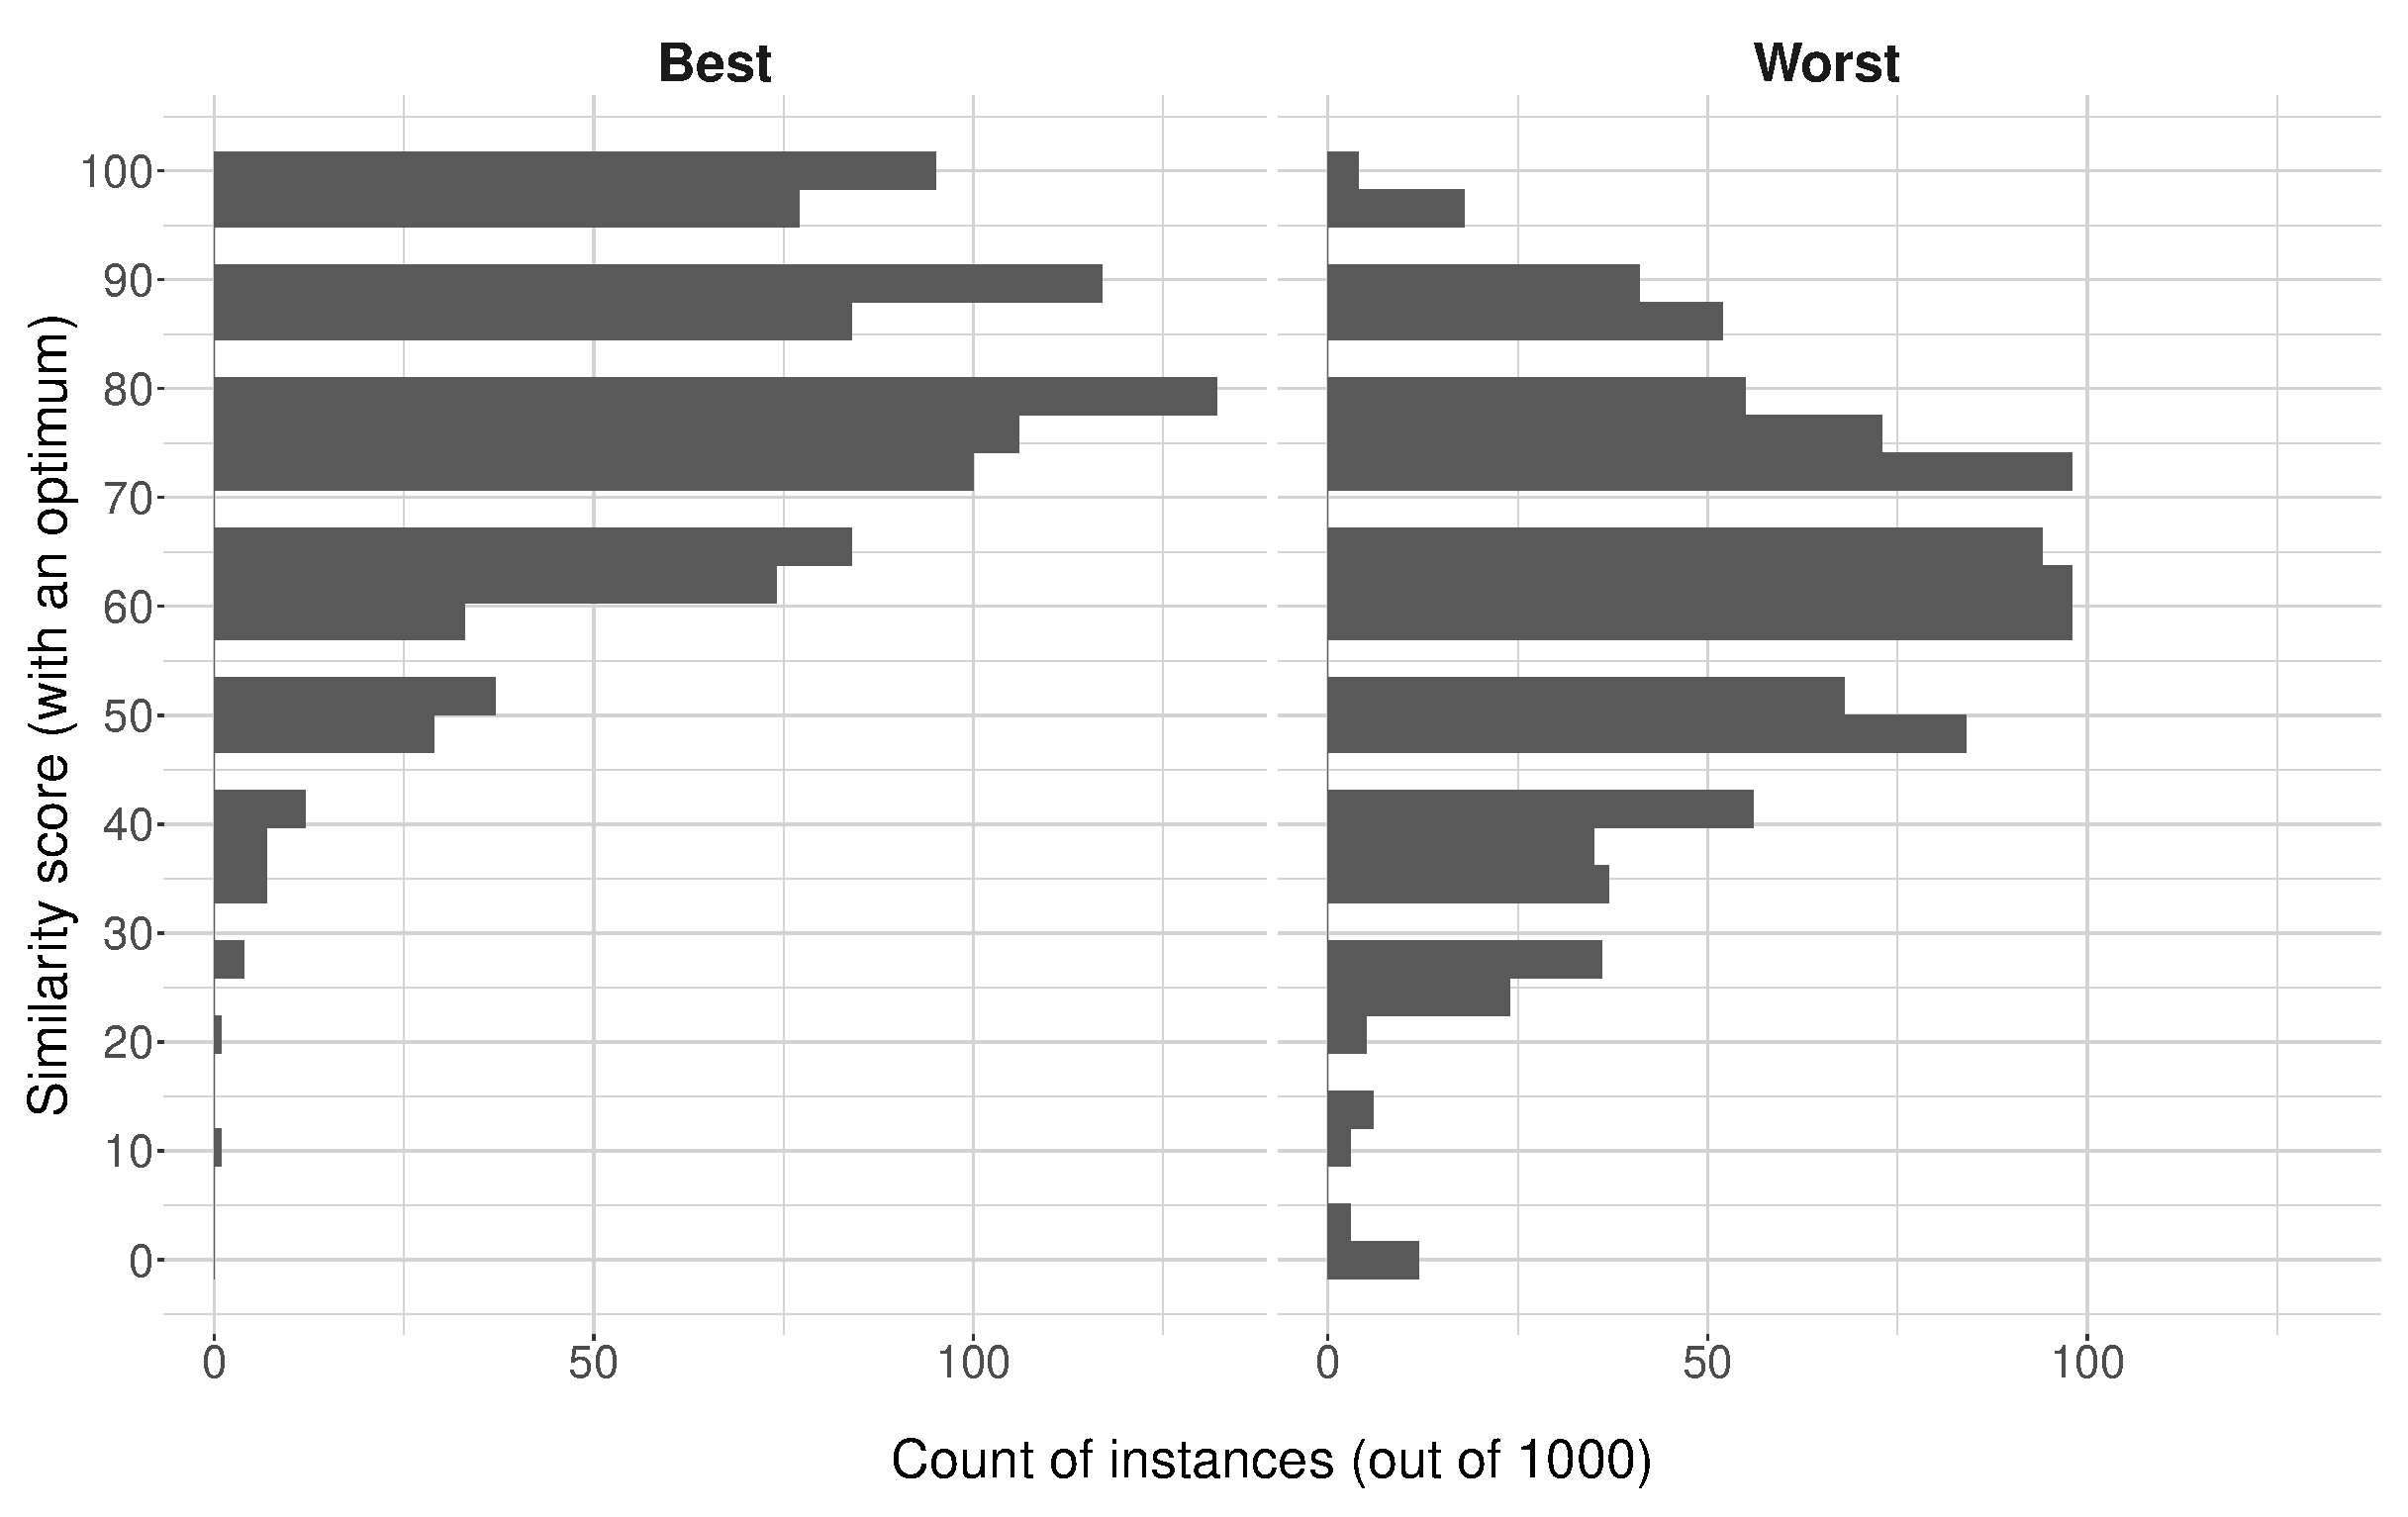
\includegraphics[width=\textwidth]{./img/heuristic_simscore.eps}
\end{frame}
\begin{frame}[label={sec:orgb6b3280}]{Effects of the problem structure}
\centering
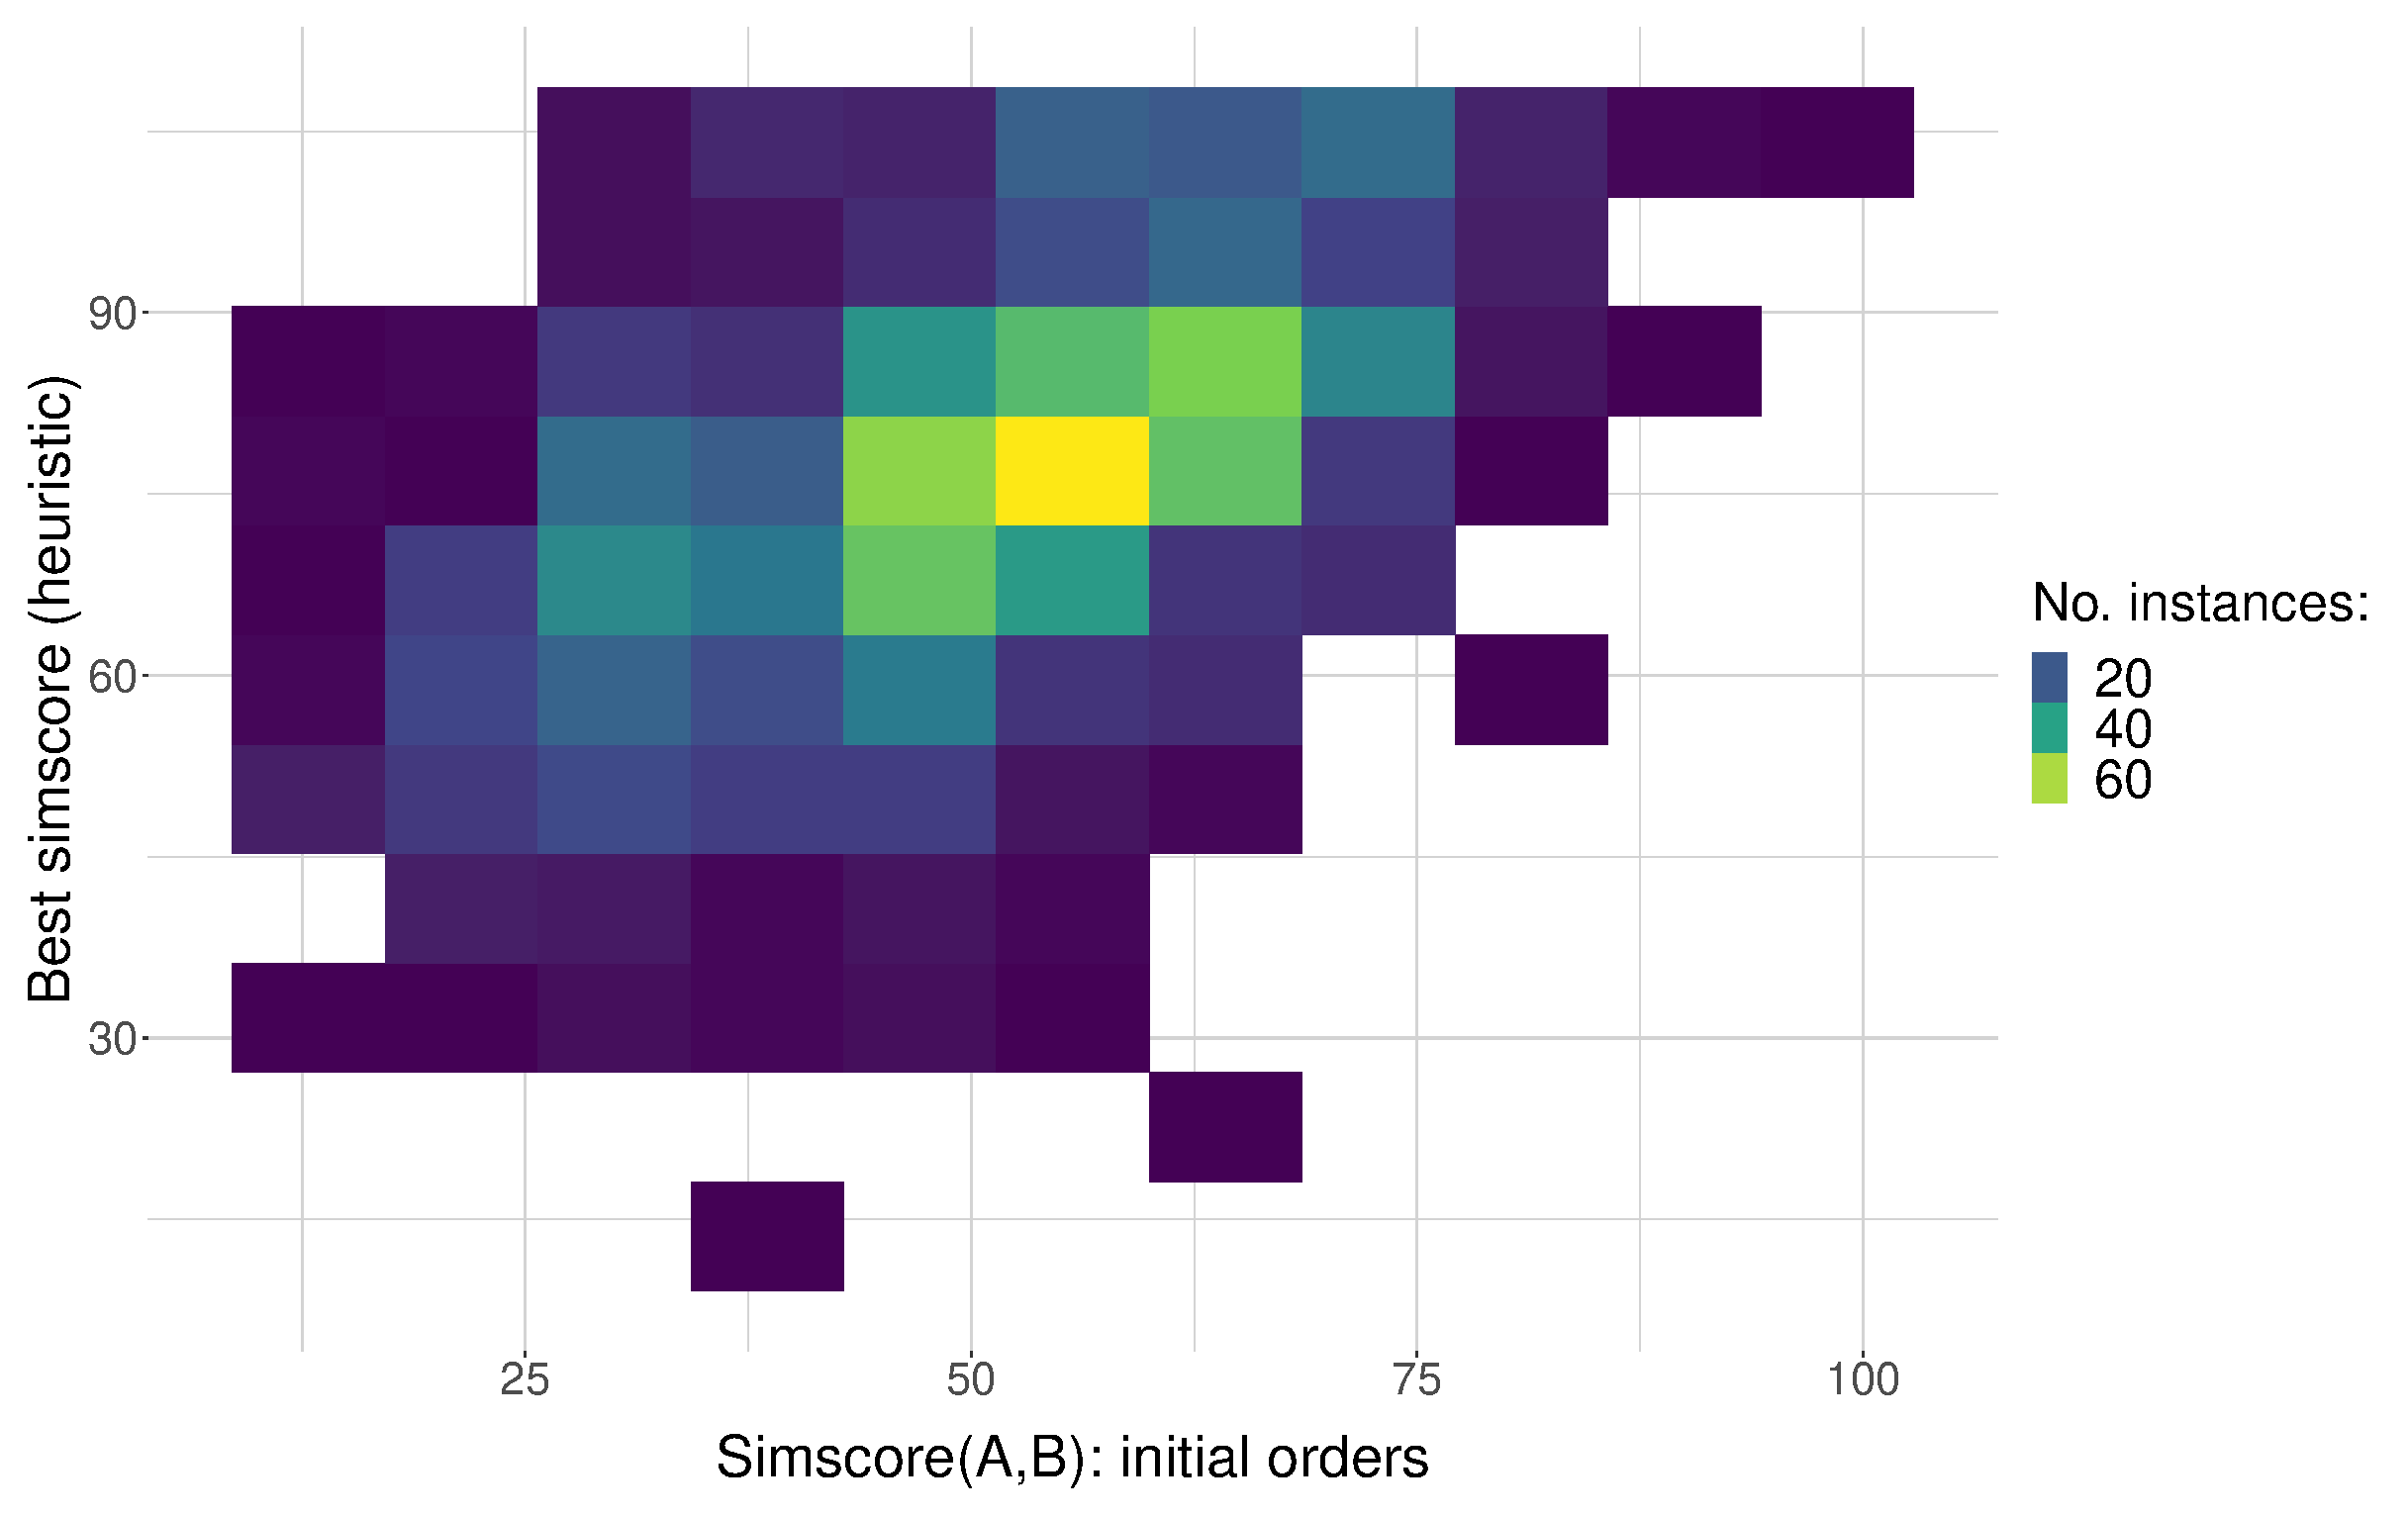
\includegraphics[width=\textwidth]{./img/heuristic_simscore_vs_AB_simscore.eps}
\end{frame}
\section[BDDs for t-UFLP]{A BDD-based approach to a Facility Location Problem}
\label{sec:org63df940}
\subsection*{Section outline}
\label{sec:orge2155c4}
\tableofcontents[currentsection]
\subsection{Problem description}
\label{sec:org5fd2bf1}
\begin{frame}[label={sec:org5670909}]{A variant of the Facility Location Problem}
\begin{columns}
\begin{column}{0.5\columnwidth}
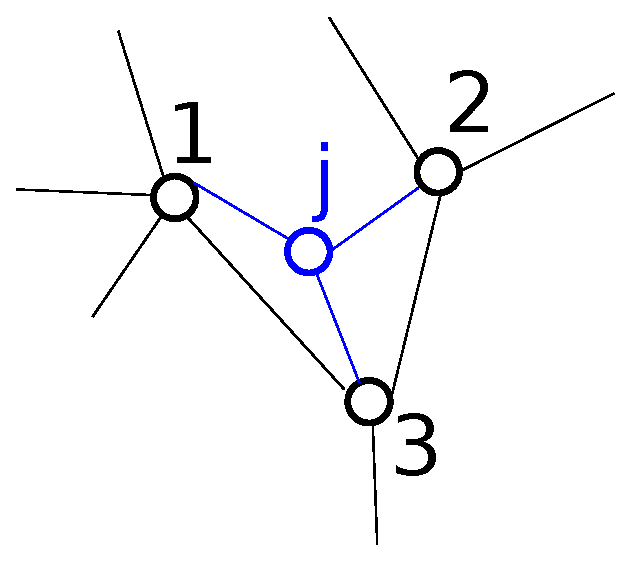
\includegraphics[width=\textwidth]{img/cover-graph.eps}
\end{column}

\begin{column}{0.5\columnwidth}
\begin{itemize}
\item \alert{Locate} facilities in a cheapest way, \ldots{}
\item \ldots{} to \alert{cover} all points, \ldots{}
\item \ldots{} respecting the \alert{budget} constraints, by facility ``type''.
\end{itemize}
\end{column}
\end{columns}
\end{frame}
\subsection{BDD representation}
\label{sec:org445b977}
\begin{frame}[label={sec:orgb447907}]{Problem formulation}
\begin{columns}
\begin{column}{0.7\columnwidth}
\begin{flalign*}
  \min & \sum_{i=1}^M f_i x_i&&\\
    \textrm{s.t. } & \sum_{j\in S_i}x_j  \geq 1 & i=1,\ldots,M, &\onslide<2->{\alert{\rightarrow  \textrm{ ``Cover'' BDD}}}\\
    &\sum_{j\in T_t}x_j  \leq k_t & t=1,\ldots, K,&\onslide<2->{\alert{\rightarrow \textrm{ ``Type'' BDD}}}\\
    & x_i\in\{0,1\} &i=1,\ldots,M. &
\end{flalign*}
\end{column}
\begin{column}{0.3\columnwidth}
Here:
\begin{itemize}
\item \(S_j\) -- adjacency lists,
\item \(k_t\) -- budgets,
\item \(f_i\) -- location costs,
\item \(x_i\) -- location decisions.
\end{itemize}
\end{column}
\end{columns}
\end{frame}
\begin{frame}[label={sec:orgd139457},t]{How to build the cover BDD}
\begin{columns}
\begin{column}[t]{0.3\columnwidth}
\centering
Original graph:\vspace{2ex}

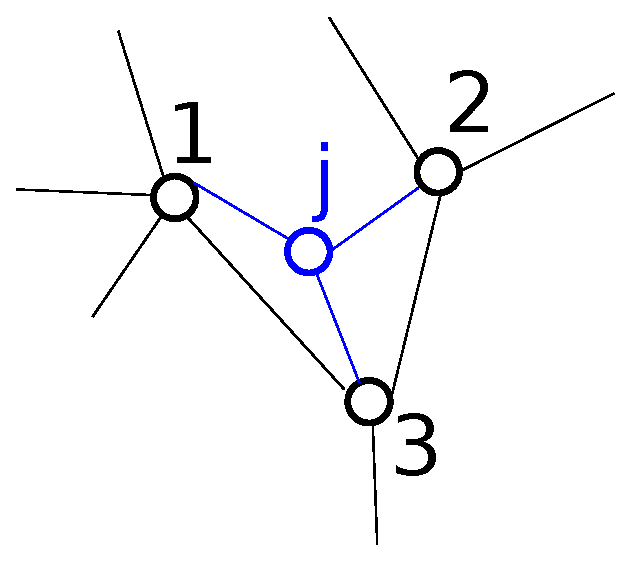
\includegraphics[width=\textwidth]{img/cover-graph.eps}
\end{column}
\begin{column}[t]{0.7\columnwidth}
\centering
Cover BDD:\vspace{2ex}

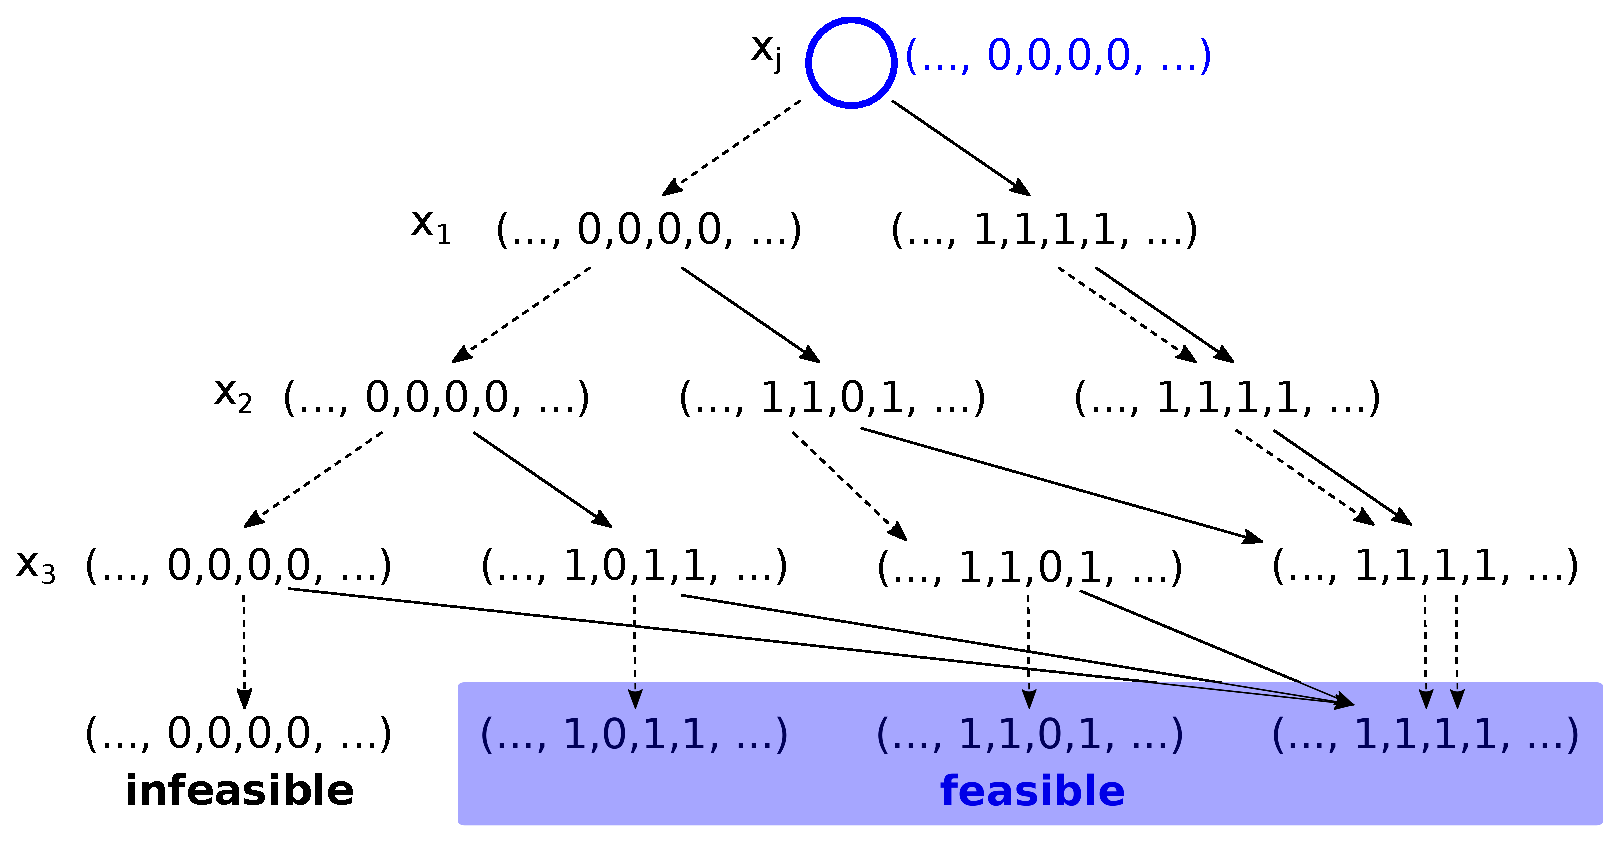
\includegraphics[width=\textwidth]{img/cover-DD.eps}
\end{column}
\end{columns}

\vspace{2ex}
\textbf{Building the diagram:}
\begin{itemize}
\item Pick next point with the least ``uncertainty'': \# of neighbors to be added to the BDD,
\item Process its adjacency list,
\item Repeat.
\end{itemize}
\end{frame}
\begin{frame}[label={sec:org2c46b26},t]{How to build the type BDD}
\begin{columns}
\begin{column}[t]{0.5\columnwidth}
\centering
Part of Type BDD:\vspace{2ex}

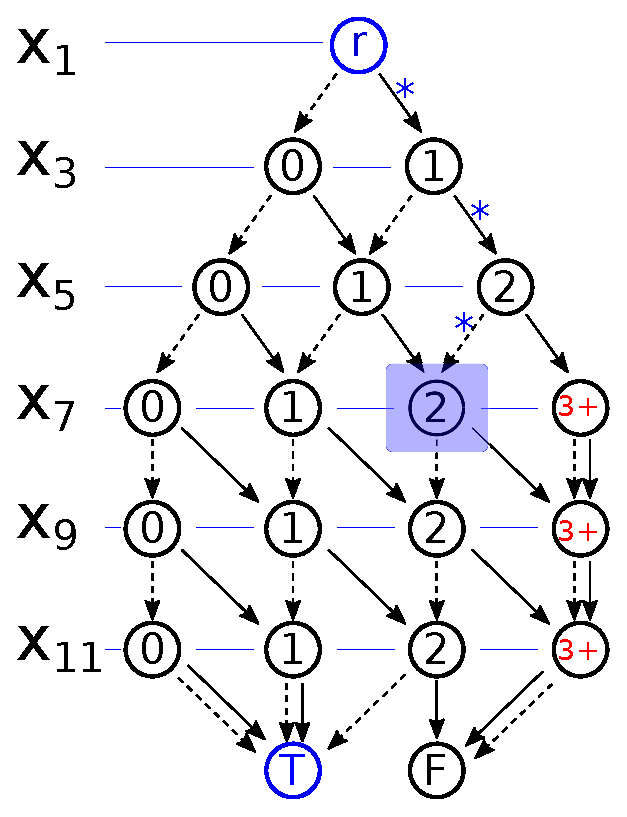
\includegraphics[height=0.7\textheight]{img/type_DD.eps}
\end{column}
\begin{column}[t]{0.5\columnwidth}
\begin{itemize}
\item Consider: \(\sum_{j\in T}x_j \leq k\) for \(T=\{1,3,5,7,9,11\}\) and \(k=2\).
\item Stack such blocks vertically.
\item Minimize the number of inversions with the Cover BDD by choosing the
order of variables within each block.
\item Randomize the order of blocks.
\end{itemize}
\end{column}
\end{columns}
\end{frame}
\begin{frame}[label={sec:orgf612a46}]{Consistent Path Problem for t-UFLP}
\begin{subequations}
\scriptsize
  \begin{align*}
    \min & \sum \tikzmarkin<2>{obj}f_i v^{\cov}_{i,\hi{i}}\tikzmarkend{obj},\\
    \textrm{s.t. } & \tikzmarkin<3>{a}(3.5,-0.5)(-0.1,0.35)\sum_{i:\hi{i}=u\textrm{ or }\lo{i}=u}v^{\cov}_{iu} = \sum_{j:\hi{u}=j\textrm{ or } \lo{u}=j}v^{\cov}_{uj} \textrm{ for all } u\in L_2^{\cov}\cup\ldots\cup L_{(M-1)}^{\cov},\\
         & \sum_{j:\hi{\ROOT}=j\textrm{ or } \lo{\ROOT}=j}v^{\cov}_{\ROOT{}j} = 1,\\
         & \sum_{j:\hi{j}=u\textrm{ or } \lo{j}=u}v^{\cov}_{ju} = 1 \textrm{ for } u\in \{\T^{\cov},\F^{\cov}\},\tikzmarkend{a}\\
         & \tikzmarkin<4>{b}(3.5,-0.5)(-0.1,0.35)\sum_{i:\hi{i}=u\textrm{ or }\lo{i}=u}v^{\type}_{iu} = \sum_{j:\hi{u}=j\textrm{ or } \lo{u}=j}v^{\type}_{uj} \textrm{ for all } u\in L_2^{\type}\cup\ldots\cup L_{(M-1)}^{\type},\\
         & \sum_{j:\hi{\ROOT}=j\textrm{ or } \lo{\ROOT}=j}v^{\type}_{\ROOT{}j} = 1,\\
         & \sum_{j:\hi{j}=u\textrm{ or } \lo{j}=u}v^{\type}_{ju} = 1 \textrm{ for } u\in \{\T^{\type},\F^{\type}\},\tikzmarkend{b}\\
         &\tikzmarkin<5>{c}(0.1,-0.5)(-0.1,0.3) \sum_{j\in L^{\cov}_q} v^{\cov}_{j\hi{j}} = x_q \textrm{ for all } q=1,\ldots,M,\\
         & \sum_{j\in L^{\type}_q} v^{\type}_{j\hi{j}} = x_q \textrm{ for all } q=1,\ldots,M,\tikzmarkend{c}\\
         & v_{pq}\geq 0 \textrm{ for all valid } p,~q;\quad x_i\in\{0,1\}.
  \end{align*}
\end{subequations}
\end{frame}

\subsection{Solving the CPP}
\label{sec:orgf678273}
\begin{frame}[label={sec:orgb705f8e}]{Approaches to solve the problem}
\begin{itemize}
\item Simple MIP (with \(x_i\in\{0,1\}\) as decision variables),
\item CPP + MIP (with continuous BDD flows + \(x_i\) as variables),
\item CPP \(\rightarrow\) Align-BDD \(\rightarrow\) shortest-path (no binary variables!)
\end{itemize}
\end{frame}
\subsection{Numerical experiments}
\label{sec:org4842d8d}
\begin{frame}[label={sec:org1dfff9f}]{Comparing runtimes (random instances)}
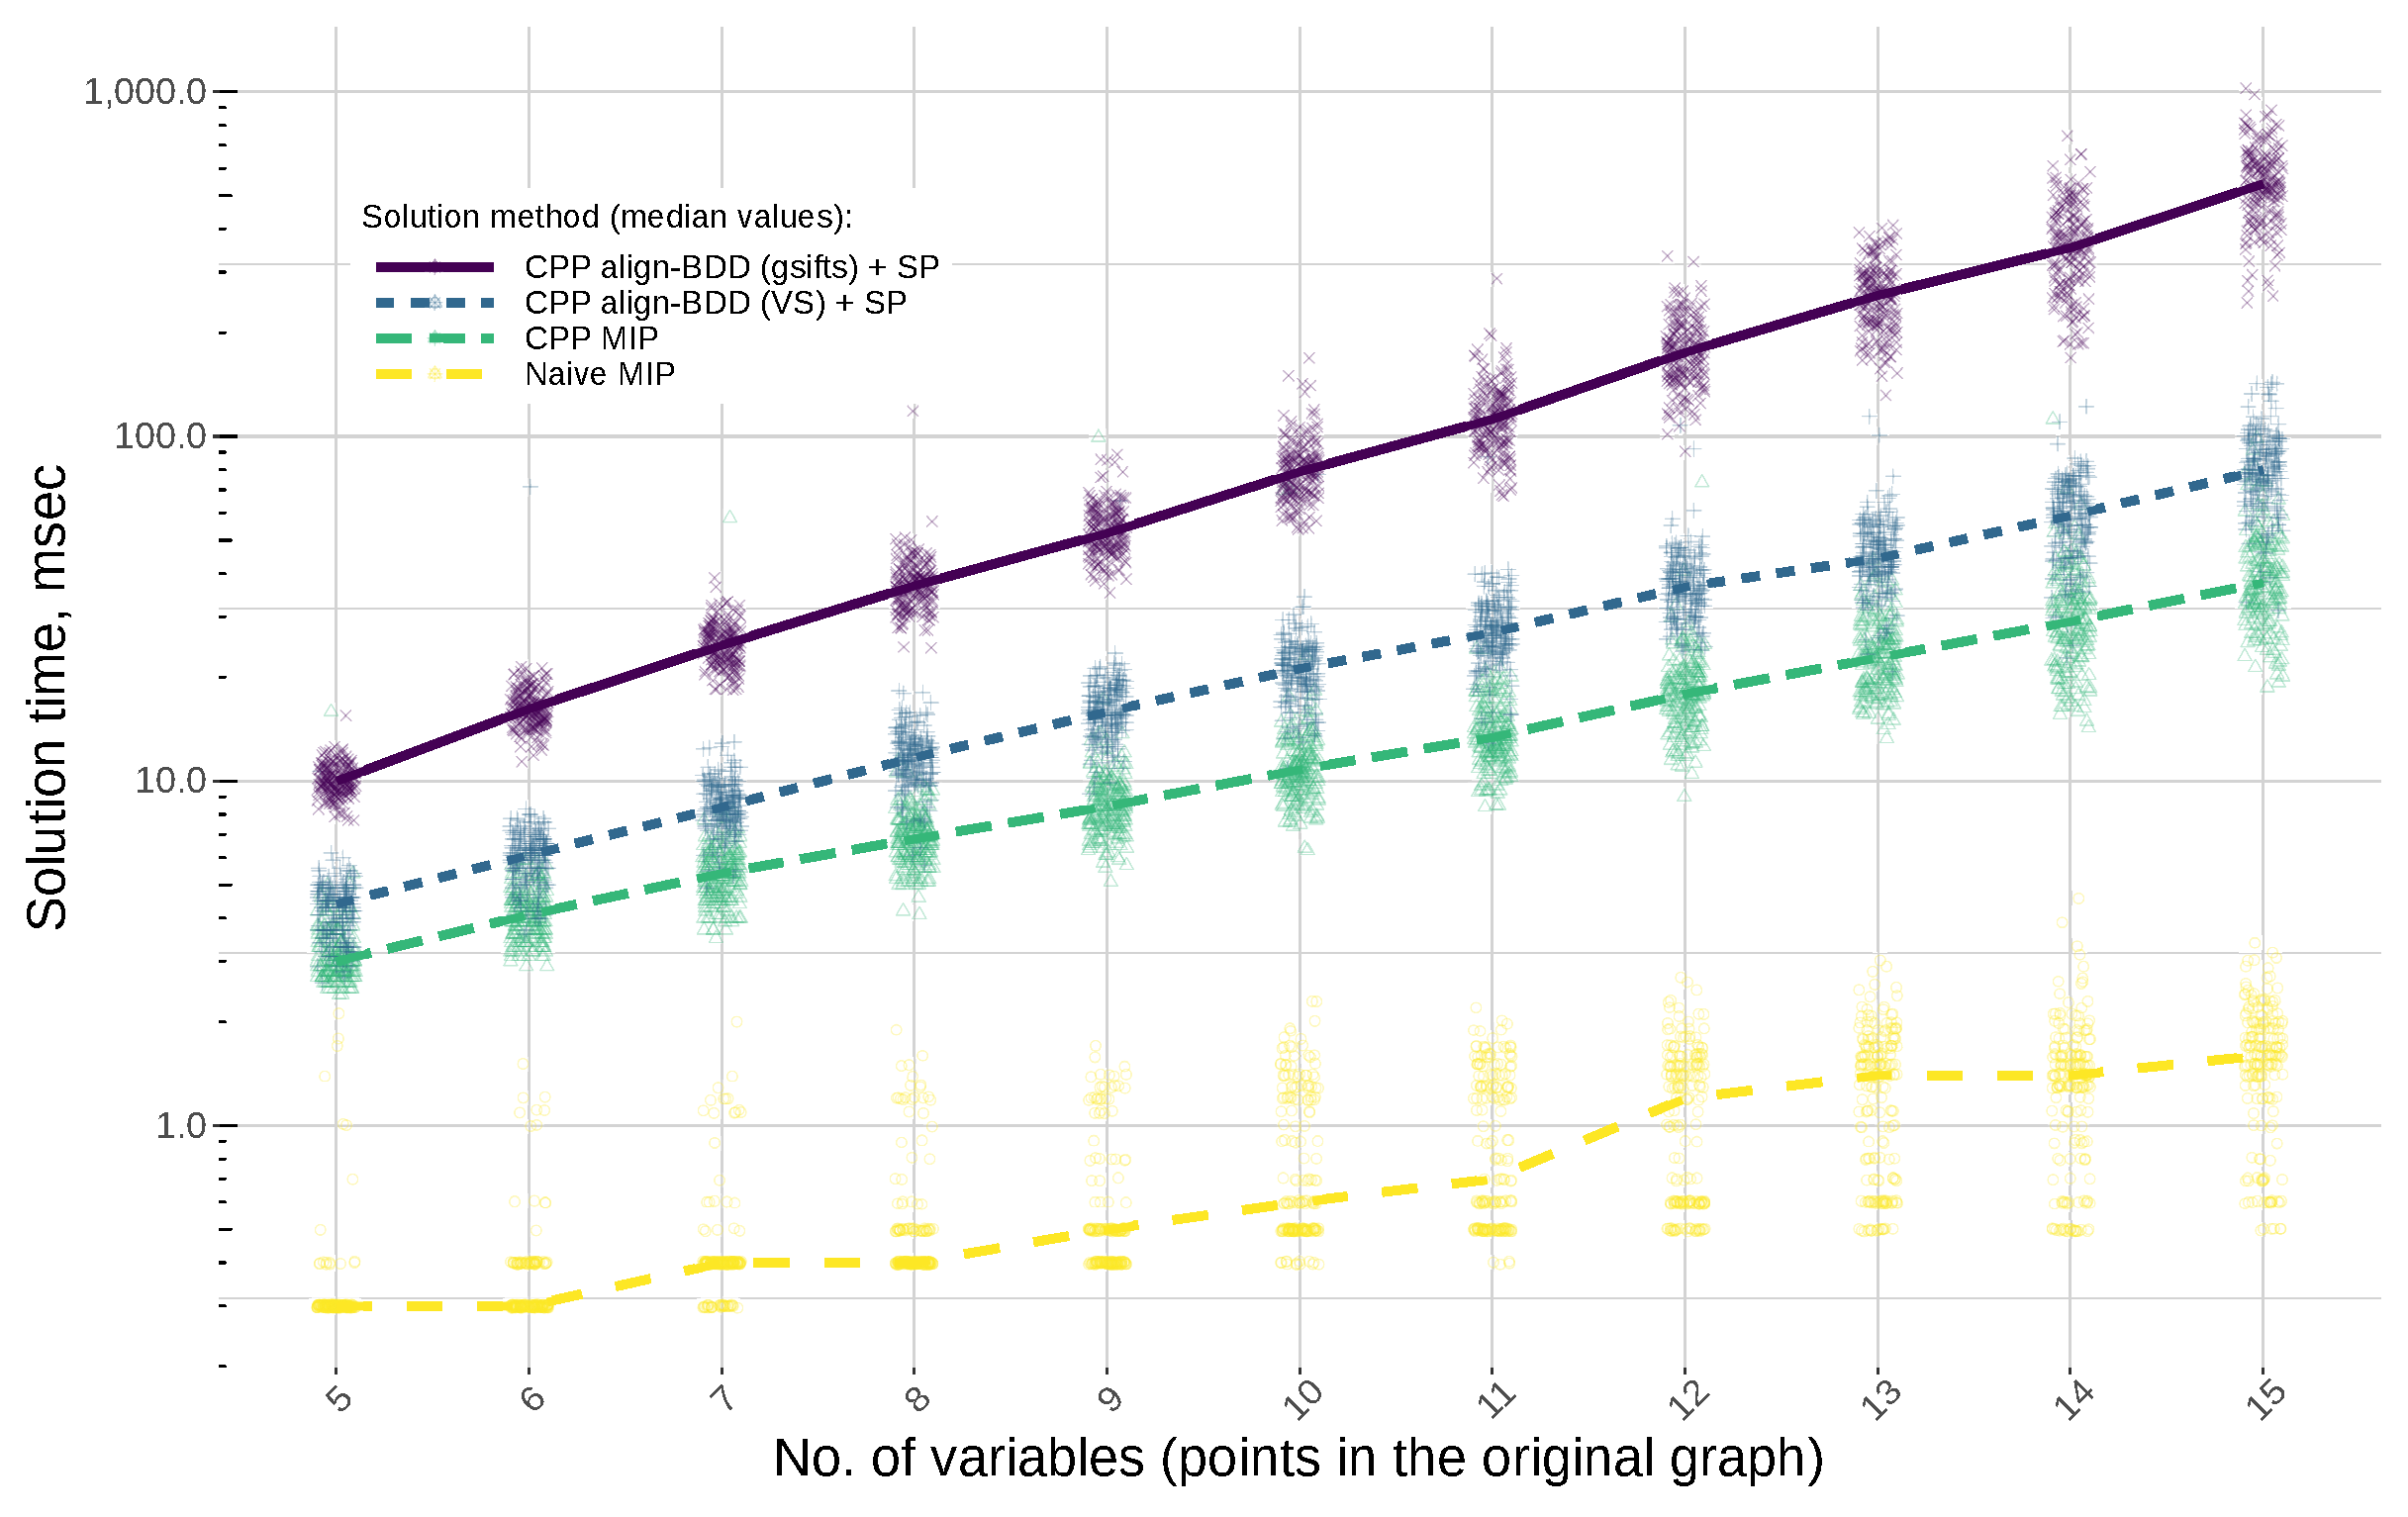
\includegraphics[width=\textwidth]{./img/tUFLP_runtimes_overview.eps}
\end{frame}
\begin{frame}[label={sec:org45cc5c6}]{Runtimes breakdown}
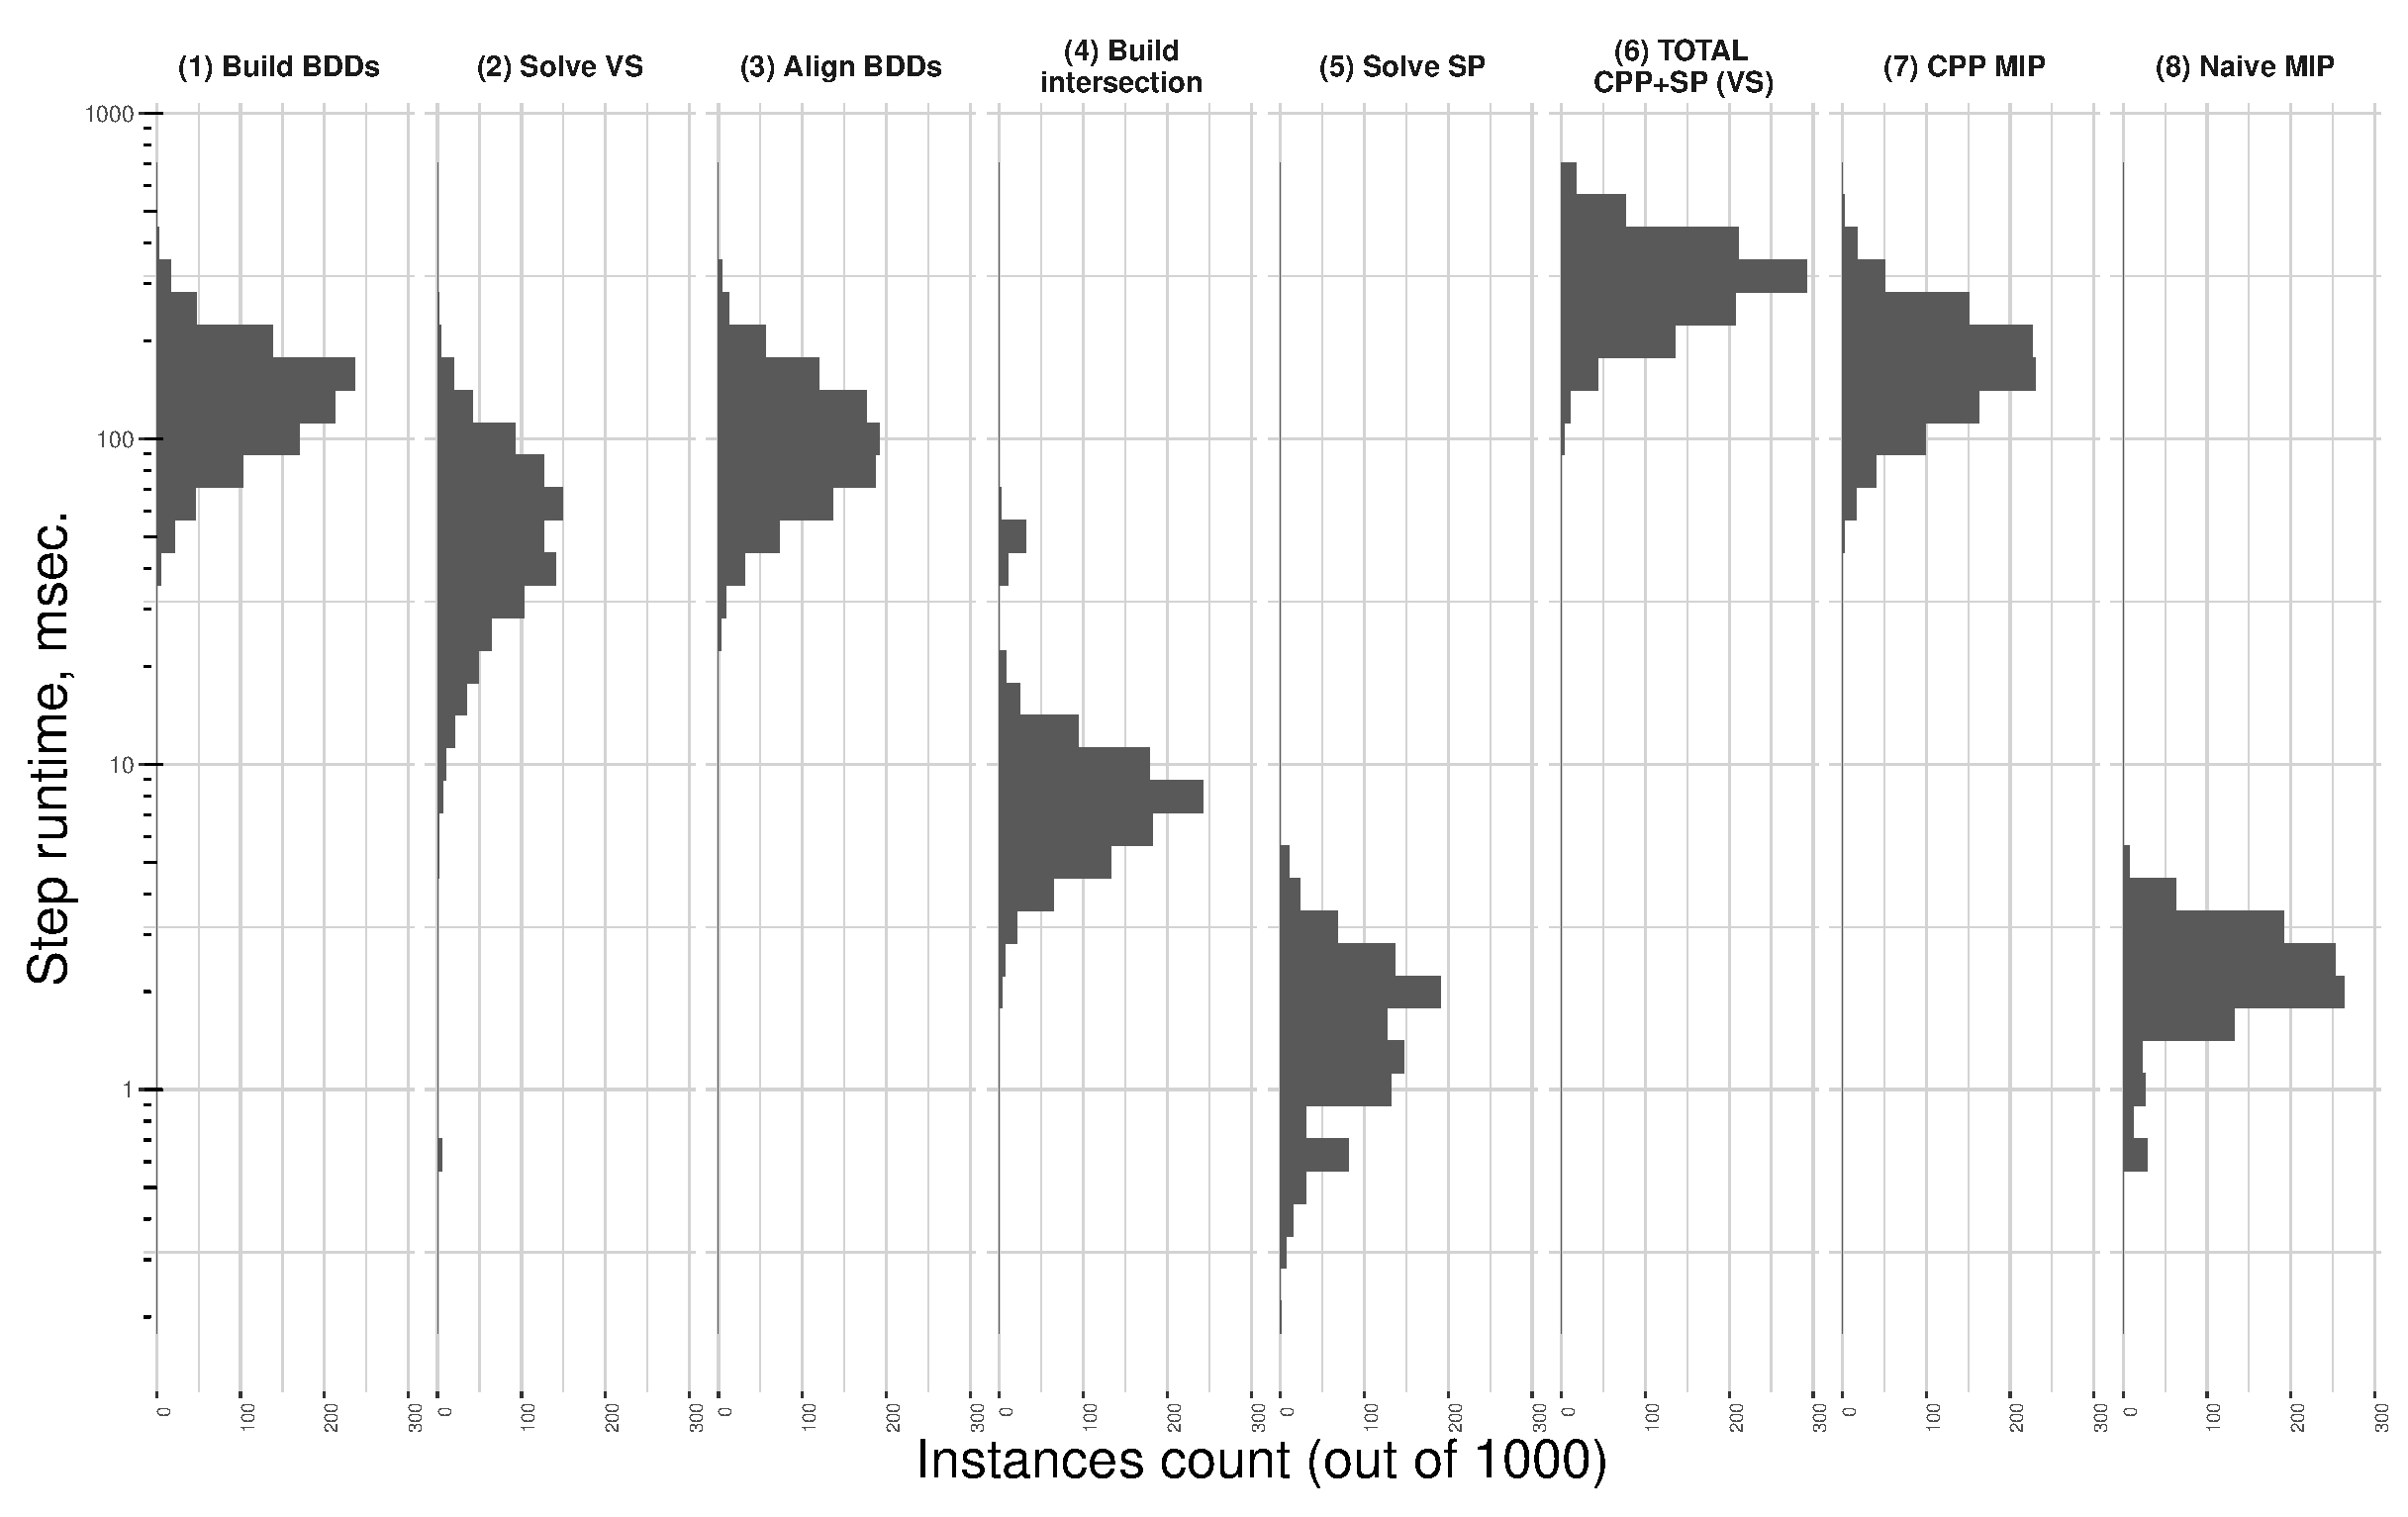
\includegraphics[width=\textwidth]{./img/tUFLP_runtimes_breakdown.eps}
\end{frame}
\begin{frame}[label={sec:org4fa9fd1}]{Alignment heuristic performance vs. problem structure}
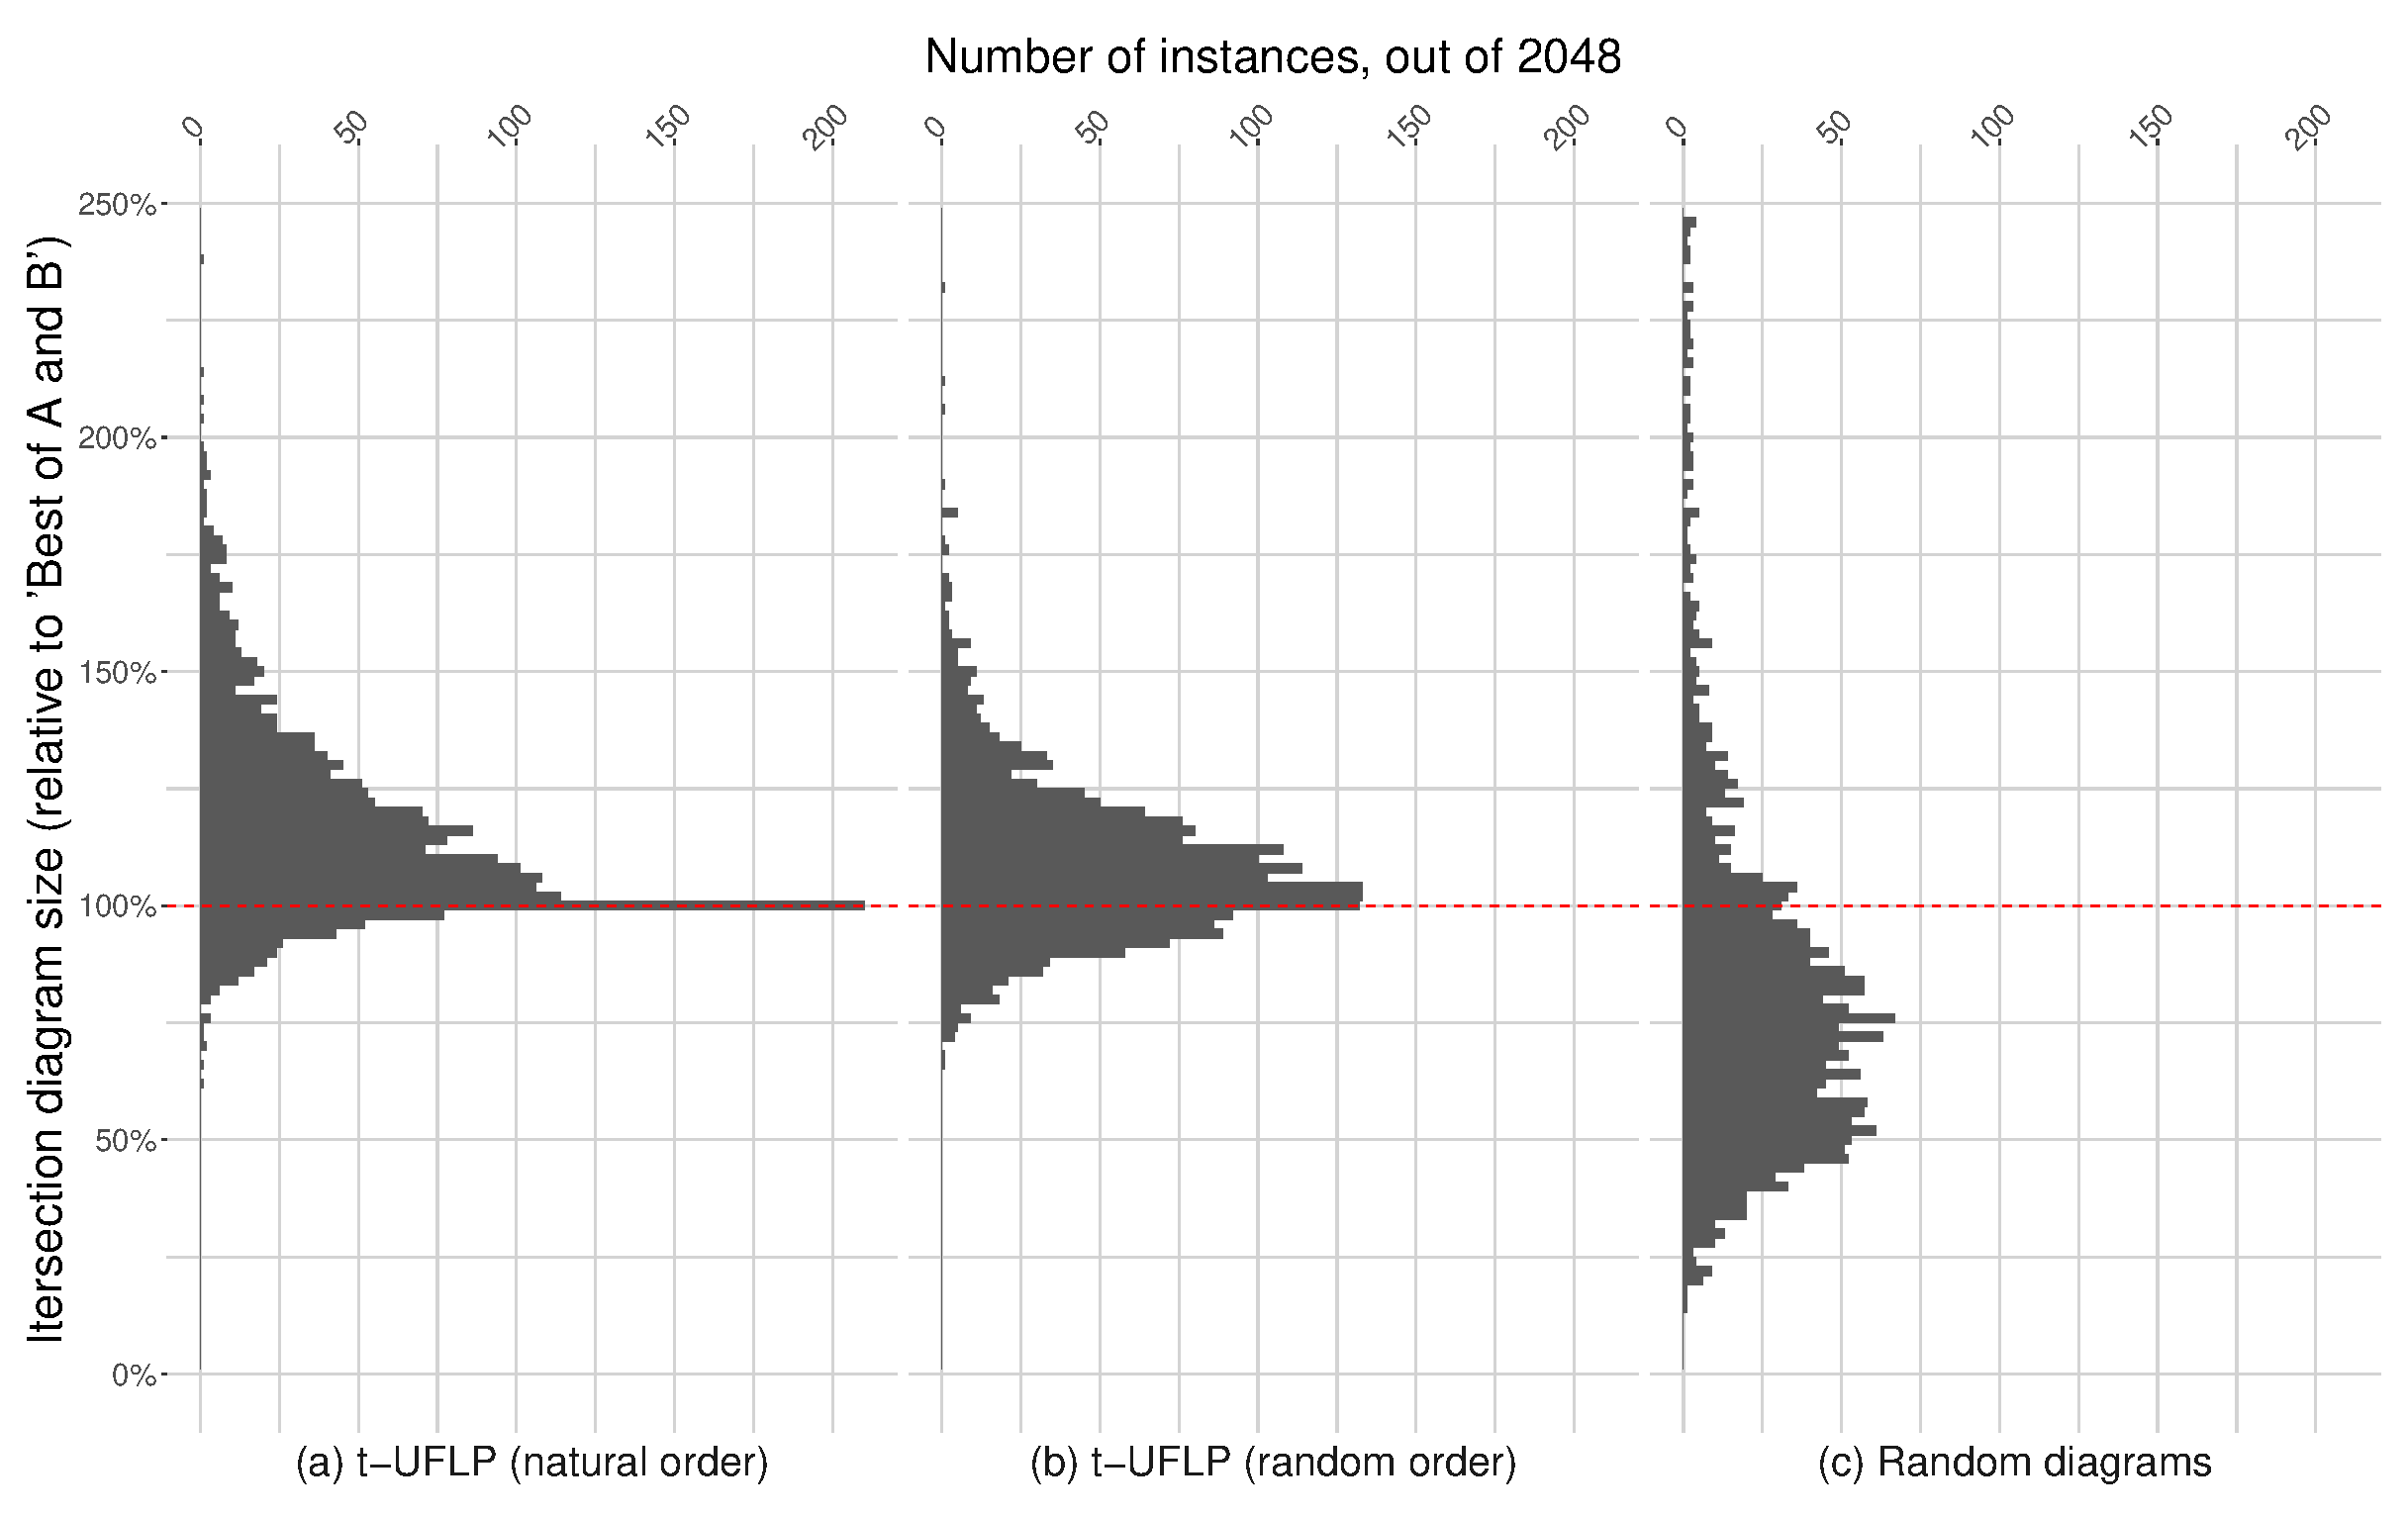
\includegraphics[width=\textwidth]{./img/various_simpl_vs_min.eps}
\end{frame}
\subsection*{t-UFLP summary}
\label{sec:orgb0129f5}
\begin{frame}[label={sec:org801f74a}]{Summary on t-UFLP}
\begin{itemize}
\item present an illustration for the Align-BDD heuristic (simplified problem),
\item introduce a problem, propose a CPP reformulation,
\item apply the heuristic to align the diagrams and obtain an LP,
\item demonstrate the runtimes in numerical experiments,
\item highlight the limits / effects of the problem structure.
\end{itemize}
\end{frame}

\section{Monte Carlo Tree Search for DSPI}
\label{sec:orgcd44ecb}
\subsection*{Section outline}
\label{sec:org1c8151f}
\tableofcontents[currentsection]
\subsection{Problem formulation}
\label{sec:orgc1d06ba}
\begin{frame}[label={sec:org2b30a3c}]{A game of ``interdiction'': intro}
\begin{columns}
\begin{column}[t]{0.4\columnwidth}
\begin{center}
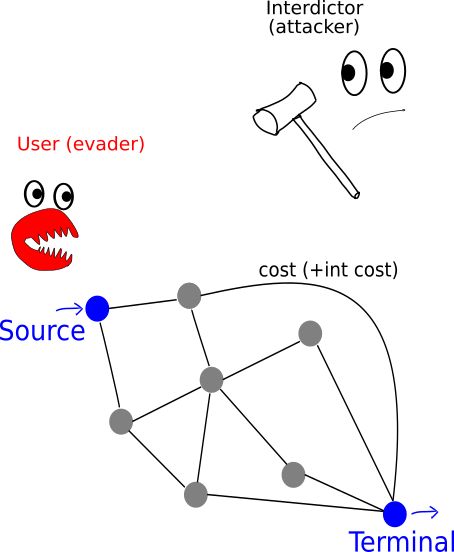
\includegraphics[width=.9\linewidth]{./img/SPI.png}
\end{center}
\end{column}

\begin{column}[t]{0.6\columnwidth}
\begin{itemize}
\item \alert{Network:} a directed graph with two special nodes (source \textcircled{s} and terminal \textcircled{t}), and a pair of "costs" associated to each edge.
\item \alert{User:} seeks to run through the graph, \textcircled{s} to \textcircled{t}, at min cost.
\item \alert{Attacker:} maximizes the User's cost by "attacking" the arcs, having a limited "budget".
\end{itemize}

We consider a \alert{dynamic} version of the game, following \cite{sefair2016}. (NP-hard)
\end{column}
\end{columns}
\end{frame}

\begin{frame}[label={sec:orgdd2493a}]{A game of ``interdiction'': formulation}
The Interdictor's optimal objective \(z^*\) can be expressed as:
\begin{equation*}
z^*(S,i) = \max_{S^\prime \subseteq \FS{i}\setminus S~:~|S\cup S^\prime|\leq b} \Big\{\min_{j\in\FS{i}} \{z^*(S\cup S^\prime, j) + \widetilde{c}_{ij}(S\cup S^\prime)\}\Big\},
\end{equation*}
where:
\begin{itemize}
\item \(S\): interdiction set,
\item \(i\): current Evader's node, \(\FS{i}\) -- forward star of node \(i\),
\item \(\widetilde{c}_{ij}\): arc traversal costs (given the interdiction),
\item \(b\): Interdictor's budget.
\end{itemize}
\pause

\begin{block}{Existing algorithms (by Sefair \& Smith)}
\begin{itemize}
\item polynomial DP algorithm for a DAG
\item exact DP algorithm, exp time for general case.
\end{itemize}
\end{block}
\end{frame}
\subsection*{What do we propose?}
\label{sec:org7704484}
\begin{frame}[label={sec:orgcd539e7}]{Monte Carlo Tree Search}
\begin{itemize}
\item Maintain the game tree,
\item Try not to create all the nodes,
\item Prune the definitely suboptimal ones,
\item Drive the tree growth by a computationally cheap objective estimate (e.g.,
based on simulated games).
\end{itemize}
\end{frame}

\subsection{MCTS framework}
\label{sec:org093231a}
\begin{frame}[label={sec:orge6b0aff}]{The ``game tree''}
Create a ``game tree'', where \alert{nodes} contain the following information.
\begin{itemize}
\item Current \alert{status}
\begin{itemize}
\item \(\pos{j}\in \mathcal{N}\): where is the Evader,
\item \(S_j\subseteq \mathcal{A}\): what is interdicted,
\item \(\tau(j)\): who's turn is it (Interdictor/Evader)\pause
\end{itemize}
\item Possible further \alert{development}
\begin{itemize}
\item \(\children{j}\): child game tree nodes,
\item \(\actions{j}\): available actions.\pause
\end{itemize}
\item \alert{Costs} info, to drive the search and prune the tree
\begin{itemize}
\item \(\widehat{Q}_j\): cost-to-go (starting from this node),
\item \(\LB{j},~\UB{j}\): bounds on the true cost-to-go,
\item \(N_j\in\mathbb{N}\): how many times the node was visited\pause
\end{itemize}

So, we iterate through \alert{episodes}, each one implying a ``full cycle'' of the game tree update in four \alert{phases}.
\end{itemize}
\end{frame}

\tikzstyle{sel} = [minimum size=2mm, NavyBlue]
\tikzstyle{stdnode} = [draw, fill, circle, lightgray, minimum size=2mm]
\tikzstyle{empty} = [draw=none, fill=none]
\tikzstyle{rootnode} = [fill=none]
\tikzstyle{edge from parent} = [draw=lightgray]

\begin{frame}[label={sec:orge77e9ee}]{Phase 1. Selection}
\begin{minipage}{0.3\textwidth}
% selection
\begin{tikzpicture}[%level distance=5mm,
level 1/.style={level distance=10mm,sibling distance=12mm},
level 2/.style={level distance=10mm,sibling distance=7mm},
level 3/.style={level distance=10mm,sibling distance=7mm},
font=\scriptsize,inner sep=2pt,every node/.style=stdnode]

\node[NavyBlue, sel] {} % root
child {node {}
        child {node {}} 
        child {node {} 
            child {node{}} 
            child {node{}}
        }
    edge from parent }
child {node {}}
child   {[NavyBlue] node[sel] {}
            child {[black] node {}}
            child {node[sel] {}
                   edge from parent[NavyBlue]
            }
        edge from parent[NavyBlue]
        };
\end{tikzpicture}
\end{minipage}\hfill
\begin{minipage}{0.5\textwidth}
\textbf{What's happening:}
\begin{itemize}
  \item Start at the root node,
  \item Use \textit{tree policy} to choose the next node recursively...
  \item ... pruning nodes as we go, when possible ...
  \item ... until we reach a leaf.
\end{itemize}
\psep{}

\textbf{What's updated:}
\begin{itemize}
  \item Nothing in the tree.
  \item Along the way: bounds for pruning (more momentarily!) + path costs.
\end{itemize}
\end{minipage}
\end{frame}
\begin{frame}[label={sec:org5b0392b}]{Phase 2. Expansion}
% expansion
\begin{minipage}{0.3\textwidth}
\begin{tikzpicture}[%level distance=5mm,
level 1/.style={level distance=10mm,sibling distance=12mm},
level 2/.style={level distance=10mm,sibling distance=7mm},
level 3/.style={level distance=10mm,sibling distance=7mm},
font=\scriptsize,inner sep=2pt,every node/.style=stdnode]

\node[rootnode] {} % root
child {node {}
        child {node {}} 
        child {node {} 
            child {node{}} 
            child {node{}}
        }
    edge from parent }
child {node {}}
child   {node {}
            child {node {}}
            child {node {}
                child {[NavyBlue] node[sel]{} edge from parent[NavyBlue]}
                child {[NavyBlue] node[sel]{} edge from parent[NavyBlue]}
                child {[NavyBlue] node[sel]{} edge from parent[NavyBlue]}
            }
        };
\end{tikzpicture}
\end{minipage}\hfill
\begin{minipage}{0.5\textwidth}
\textbf{What's happening:}
\begin{itemize}
  \item Create child nodes for possible actions.
\end{itemize}
\psep{}

\textbf{What's updated:}
\begin{itemize}
  \item New nodes are created,
  \item UBs and LBs are calculated
\end{itemize}\psep{}

\textbf{Note:} Some inconsistencies can be introduced here, between child and parent nodes.
\end{minipage}
\end{frame}
\begin{frame}[label={sec:orgee15df8}]{Phase 3. Roll-outs}
% roll-outs
\begin{minipage}{0.3\textwidth}
\begin{tikzpicture}[%level distance=5mm,
level 1/.style={level distance=10mm,sibling distance=12mm},
level 2/.style={level distance=10mm,sibling distance=7mm},
level 3/.style={level distance=10mm,sibling distance=7mm},
font=\scriptsize,inner sep=2pt,every node/.style=stdnode]

\node[rootnode] {} % root
child {node {}
        child {node {}} 
        child {node {} 
            child {node{}} 
            child {node{}}
        }
    edge from parent }
child {node {}}
child {node {}
       child {node {}}
       child {node {}
              child {node[sel] (a1) {}
                     child {node[empty, NavyBlue] (b1) {...} edge from parent[draw=none]
                       child{node[sel, fill=none] (c1) {}
                             edge from parent[draw=none]}}}
                child {node[sel] (a2) {}
                    child {node[empty, NavyBlue] (b2) {...} edge from parent[draw=none]
                       child{node[sel, fill=none] (c2) {}
                             edge from parent[draw=none]}}}
                child {node[sel] (a3) {}
                    child {node[empty, NavyBlue] (b3) {...} edge from parent[draw=none]
                       child{node[sel, fill=none] (c3) {}
                             edge from parent[draw=none]}}}}
                             };
\draw[bend left, NavyBlue, shorten <=2pt] (a1) to (b1);
\draw[->, bend right, NavyBlue, shorten >= 2pt] (b1) to (c1);
\draw[bend right, NavyBlue, shorten <=2pt] (a2) to (b2);
\draw[->, bend left, NavyBlue, shorten >=2pt] (b2) to (c2);
\draw[bend left, NavyBlue, shorten <=2pt] (a3) to (b3);
\draw[->, bend right, NavyBlue, shorten >=2pt] (b3) to (c3);
\draw[dashed, NavyBlue, rounded corners=7] ($(c1)+(-.3,.3)$)rectangle($(c3)+(.3,-.3)$);
\node[draw=none, fill=none, yshift=-4.5mm, NavyBlue] at ($(c1)!.5!(c3)$){Terminal nodes}; 
\end{tikzpicture}%
\vspace{-2.5em}
\end{minipage}\hfill
\begin{minipage}{0.5\textwidth}
\textbf{What's happening:}
\begin{itemize}
  \item Run a random simulated game from each node,
  \item Calculate cost-to-go estimate $\widehat{Q}_j$ as the simulated game cost.
\end{itemize} \psep{}

\textbf{What's updated}
\begin{itemize}
  \item Cost-to-go for each new node.
\end{itemize}\psep{}

\textbf{Note:} We do not record the intermediate game states occured during roll-outs!
\end{minipage}
\end{frame}

\begin{frame}[label={sec:orgfbe4100}]{Phase 4. Backpropagation}
% backpropagation
\begin{minipage}{0.3\textwidth}
\begin{tikzpicture}[%level distance=5mm,
level 1/.style={level distance=10mm,sibling distance=12mm},
level 2/.style={level distance=10mm,sibling distance=7mm},
level 3/.style={level distance=10mm,sibling distance=7mm},
font=\scriptsize,inner sep=2pt,every node/.style=stdnode]

\node[sel] (d) {} % root
child {node {}
        child {node {}} 
        child {node {} 
            child {node{}} 
            child {node{}}
        }
    edge from parent }
child {node {}}
child {node[sel] (c) {}
            child {node {}}
            child {node[sel] (b) {}
                child {node{}}
                child {node{}}
                child {node[sel] (a) {}}
            }
        };

\draw[->, NavyBlue, bend right, shorten >=2pt, shorten <=2pt] (a) to (b.east);
\draw[->, NavyBlue, bend right, shorten >=2pt, shorten <=2pt] (b.north east) to (c.east);
\draw[->, NavyBlue, bend right, shorten >=2pt, shorten <=2pt] (c.north east) to (d.east);
\end{tikzpicture}
\end{minipage}\hfill
\begin{minipage}{0.5\textwidth}
\textbf{What's happening:}
\begin{itemize}
  \item Start at the selected node,
  \item Recursively update (``propagate'') node information for parents ...
  \item ... until we reach the root.
\end{itemize} \psep{}

\textbf{What's updated:}
Information in each parent node, using the child nodes:
\begin{itemize}
  \item UBs and LBs
  \item Cost-to-go estimate: the best value (given the turn).
\end{itemize}
\end{minipage}
\end{frame}

\begin{frame}[label={sec:org2dd1685}]{The Algorithm}
The algorithm can perform actions for both players. Each turn involves two
steps:\vspace{2ex}

\begin{columns}
\begin{column}[t]{0.4\columnwidth}
\textbf{Step 1.} THINK.\vspace{1ex}

We iteratively improve the tree (while we have budget):\vspace{1ex}

\textbf{FOR} \(k=1,\ldots, K\) \textbf{DO}
\begin{itemize}
\item Selection
\item Expansion
\item Roll-outs
\item Backpropagation
\end{itemize}
\textbf{END.}
\end{column}

\begin{column}[t]{0.4\columnwidth}
\textbf{Step 2.} ACT.\vspace{1ex}

\ldots{} then pick an action corresponding to the ``most
attractive'' child node of the root.
\end{column}
\end{columns}
\end{frame}

\begin{frame}[label={sec:orgfdce9d2}]{There are several secret ingredients}
\begin{figure}
\includegraphics[width=\textwidth]{img/ingredient.jpg}
\end{figure}
\end{frame}

\begin{frame}[label={sec:org4805004}]{SI-1. How to select?}
\begin{itemize}
\item \textbf{with probability $\varepsilon$}: choose at random;
\item \textbf{otherwise}, a child node with the \alert{best score}:
\end{itemize}
\begin{equation*}
R_j \defeq \underbrace{\sigma_i (\widetilde{C}_{ij} + \widehat{Q}_j)}_{\textrm{best cost-to-go}} ~~+ ~~\underbrace{C_p\sqrt{\log(N_i) / N_j}}_{\textrm{encourage exploration}}, \quad \textrm{ for all } j\in\children{i}
\end{equation*}

``Best'' here depends on the turn (the Evader will choose the smallest cost estimate, the Interdictor --- the largest).
\end{frame}
\begin{frame}[label={sec:orgbb8876e}]{SI-2. How to prune?}
We leverage the classic idea of \alert{alpha--beta pruning}:
\vspace{2ex}
\begin{columns}
\begin{column}{0.4\columnwidth}
\begin{tikzpicture}[%level distance=5mm,
level 1/.style={level distance=10mm,sibling distance=12mm},
level 2/.style={level distance=10mm,sibling distance=7mm},
level 3/.style={level distance=10mm,sibling distance=7mm},
font=\scriptsize,inner sep=2pt,
edge from parent/.style={draw=black},
every node/.style={draw, circle}]

\node[label=above:{root}]{I} % root
child {node[label=left:{$(A)$}] {E}
        child {node[label=below:{$j^{\prime\prime}$}] {I}} 
        child {node[sel, label=below:{$j^\prime$}] {I}} 
        child {node {I}} 
    edge from parent node[draw=none, left] {pass}}
child {node {I}}
child   {node[sel, label=right:{$(B)$}] {I}
            child {node {I}
                child {node[draw=none] {...}}
                child {node[draw=none] {...}}}
            child {node {I}
                child {node[draw=none] {...}}}
        edge from parent};
\end{tikzpicture}
\end{column}
\begin{column}{0.6\columnwidth}
Maintain two running numbers (bounds):
\begin{itemize}
\item \(\alpha\): the worst (minimum) alternative cost achievable by the Interdictor,
\item \(\beta\): the worst (maximum) alternative cost achievable by the Evader.
\end{itemize}
\vspace{2ex}
 \alert{Pruning condition:} \(\beta \leq \ahat_j\) or \(\bhat_j \leq \alpha\), where
\begin{itemize}
\item \(\ahat_j =\pi_n+\LB{j}\)  (Interdictor's turns), and
\item \(\bhat_j = \pi_n+\widetilde{C}_{nj} + \UB{j}\) (Evader's turns)
\end{itemize}
\end{column}
\end{columns}
\end{frame}
\begin{frame}[label={sec:org77c5c63}]{SI-3. How to back-propagate?}
Assuming the Evader's turn, and \(i\) being the current game tree node:
\begin{itemize}
\item Update the bounds:
\end{itemize}
\begin{align*}
  \UB{i} &\gets \min_{j\in\children{i}} \Big\{ \widetilde{C}_{ij}(S_i) + \UB{j} \Big\},\\
  \LB{i} &\gets \min_{j\in\children{i}} \Big\{ \widetilde{C}_{ij}(S_i) + \LB{j} \Big\}.
\end{align*}

\begin{itemize}
\item Update the cost-to-go estimate:
\end{itemize}
\begin{equation*}
\widehat{Q}_i \gets \min_{j\in\children{i}} \Big\{ \widetilde{C}_{ij}(S_i) + \widehat{Q}_j\Big\}.
\end{equation*}
\end{frame}
\begin{frame}[label={sec:org0f96b49}]{SI-4. Bounds}
Are inspired by Sefair \& Smith 2016:
\begin{itemize}
\item \textbf{Lower bound:} restrict the \alert{Attacker}. Make attacks ``expire'' after a single turn).
\item \textbf{Upper bound:} restrict the \alert{Interdictor}. Remove some arcs so that \(G\) is a DAG (\(\Rightarrow\) DSPI is simple to solve.) Repeat multiple times and choose the best bound.
\end{itemize}
\end{frame}
\subsection{Numerical experiments}
\label{sec:org72ac1bb}
\begin{frame}[label={sec:org03abae9}]{Numerical experiments: strategy}
\begin{itemize}
\item How does it perform on pre-defined instances? (relative to the known optimum, and to the bounds)
\item How does it perform on randomly generated instances with different budgets?
\item What's the dynamics of the tree construction? How does the algorithm work?
\item What's the point of ``playing out'', i.e., changing root nodes?
\end{itemize}
\end{frame}

\begin{frame}[label={sec:orgcb50a57}]{Pre-defined instances}
\begin{figure}
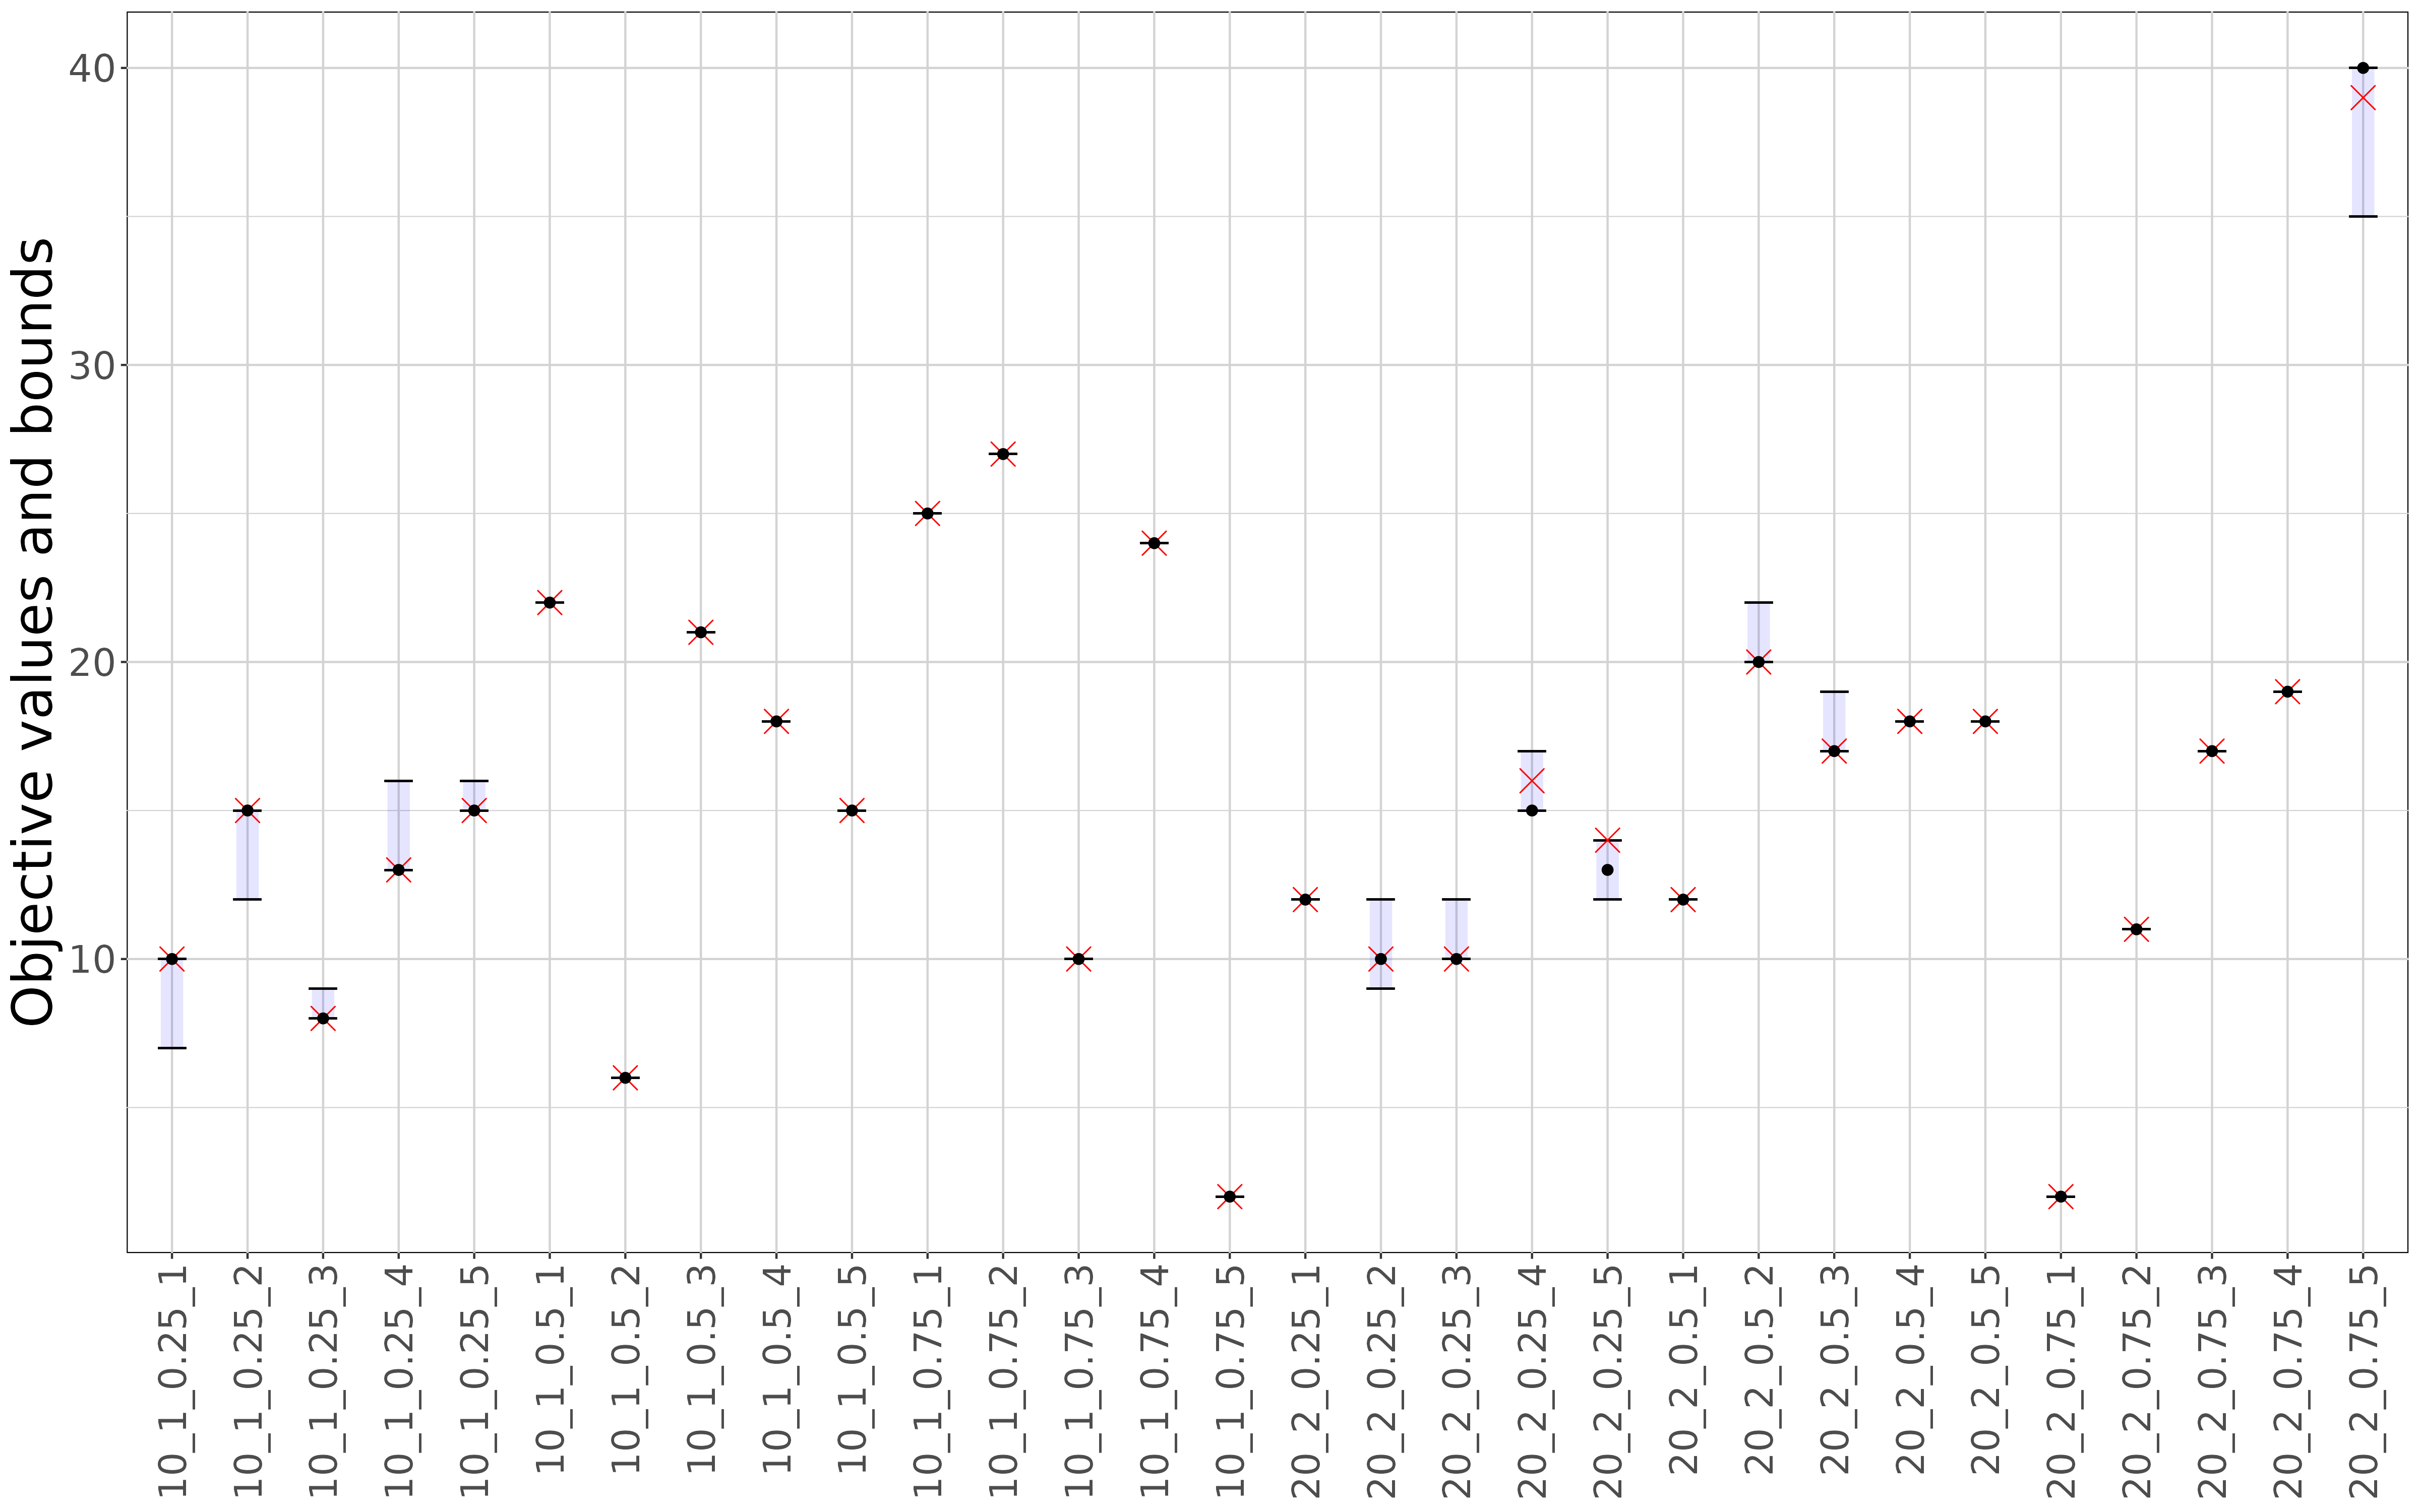
\includegraphics[width=\textwidth]{img/fig_known.png}
\end{figure}
\end{frame}
\begin{frame}[label={sec:org52aab50}]{Random instances (snapshot)}
\begin{figure}
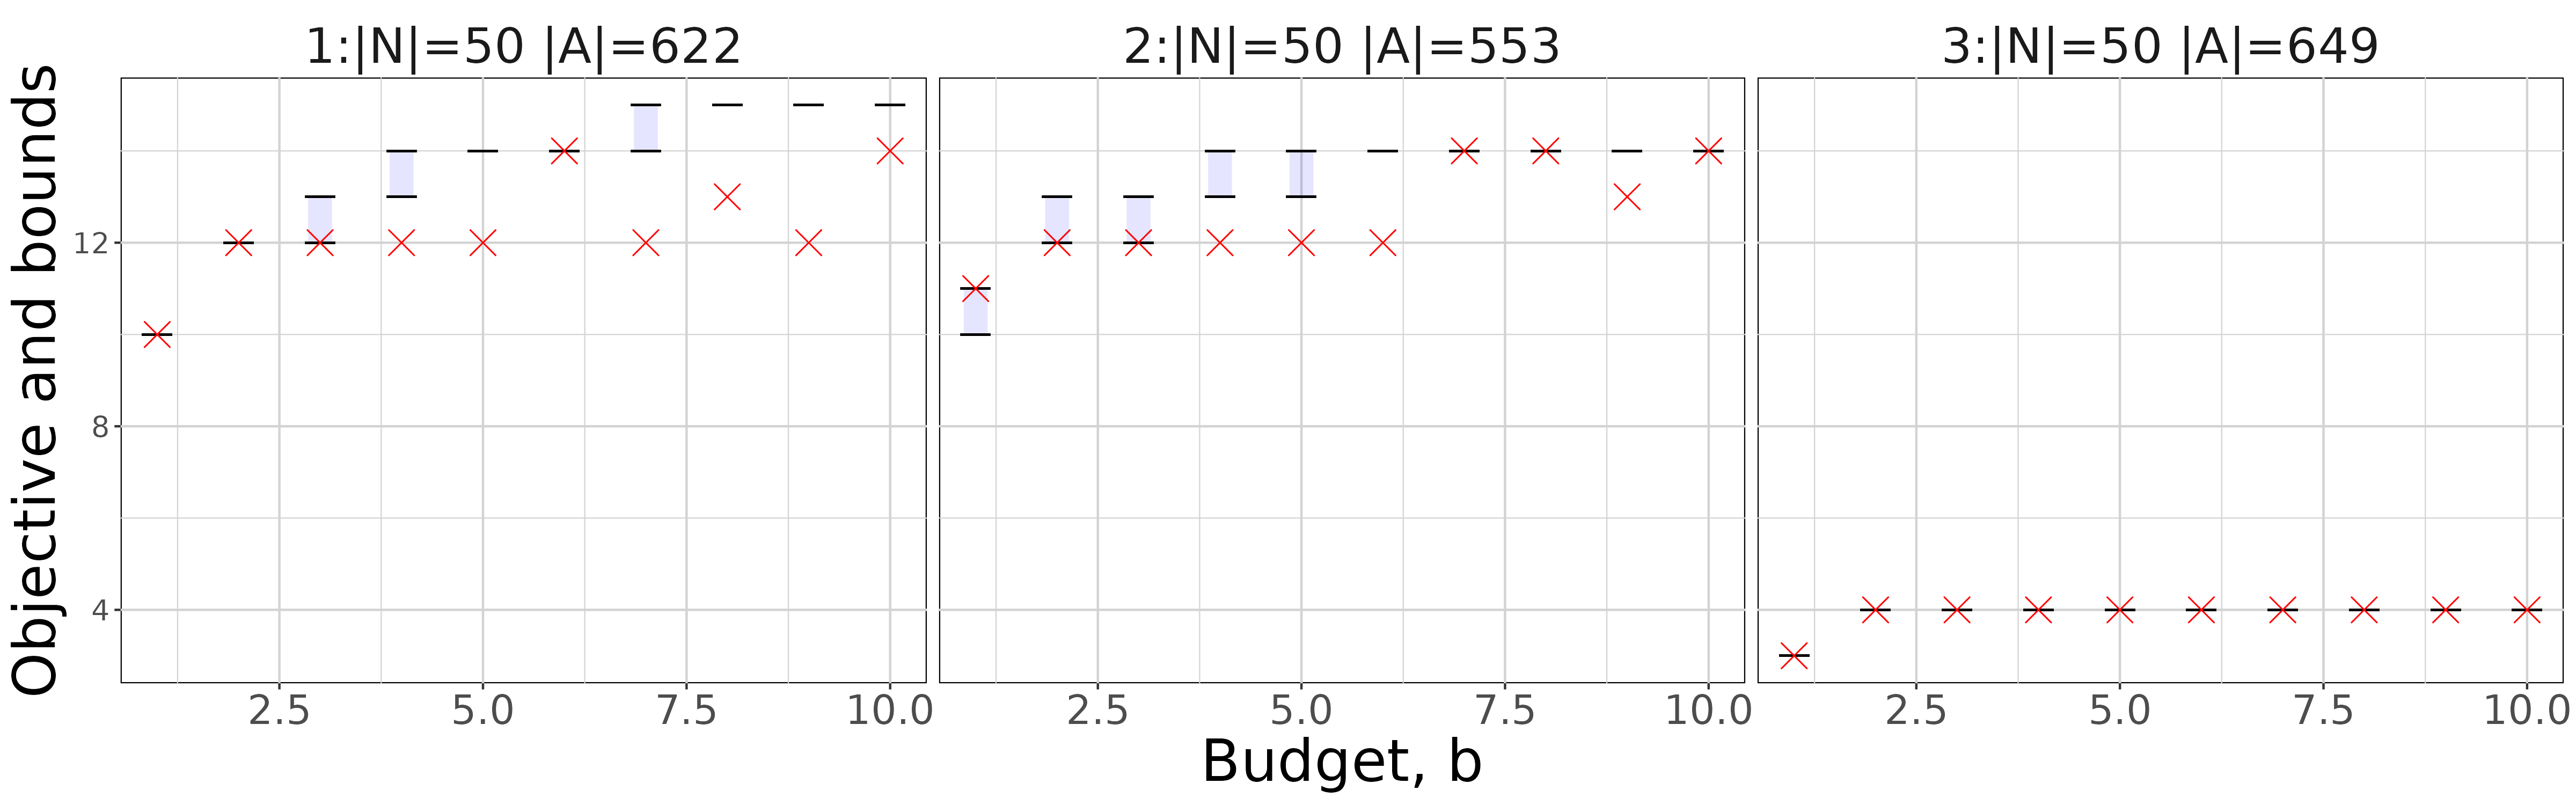
\includegraphics[width=\textwidth]{img/fig_bounds.png}\vspace{0.5ex}
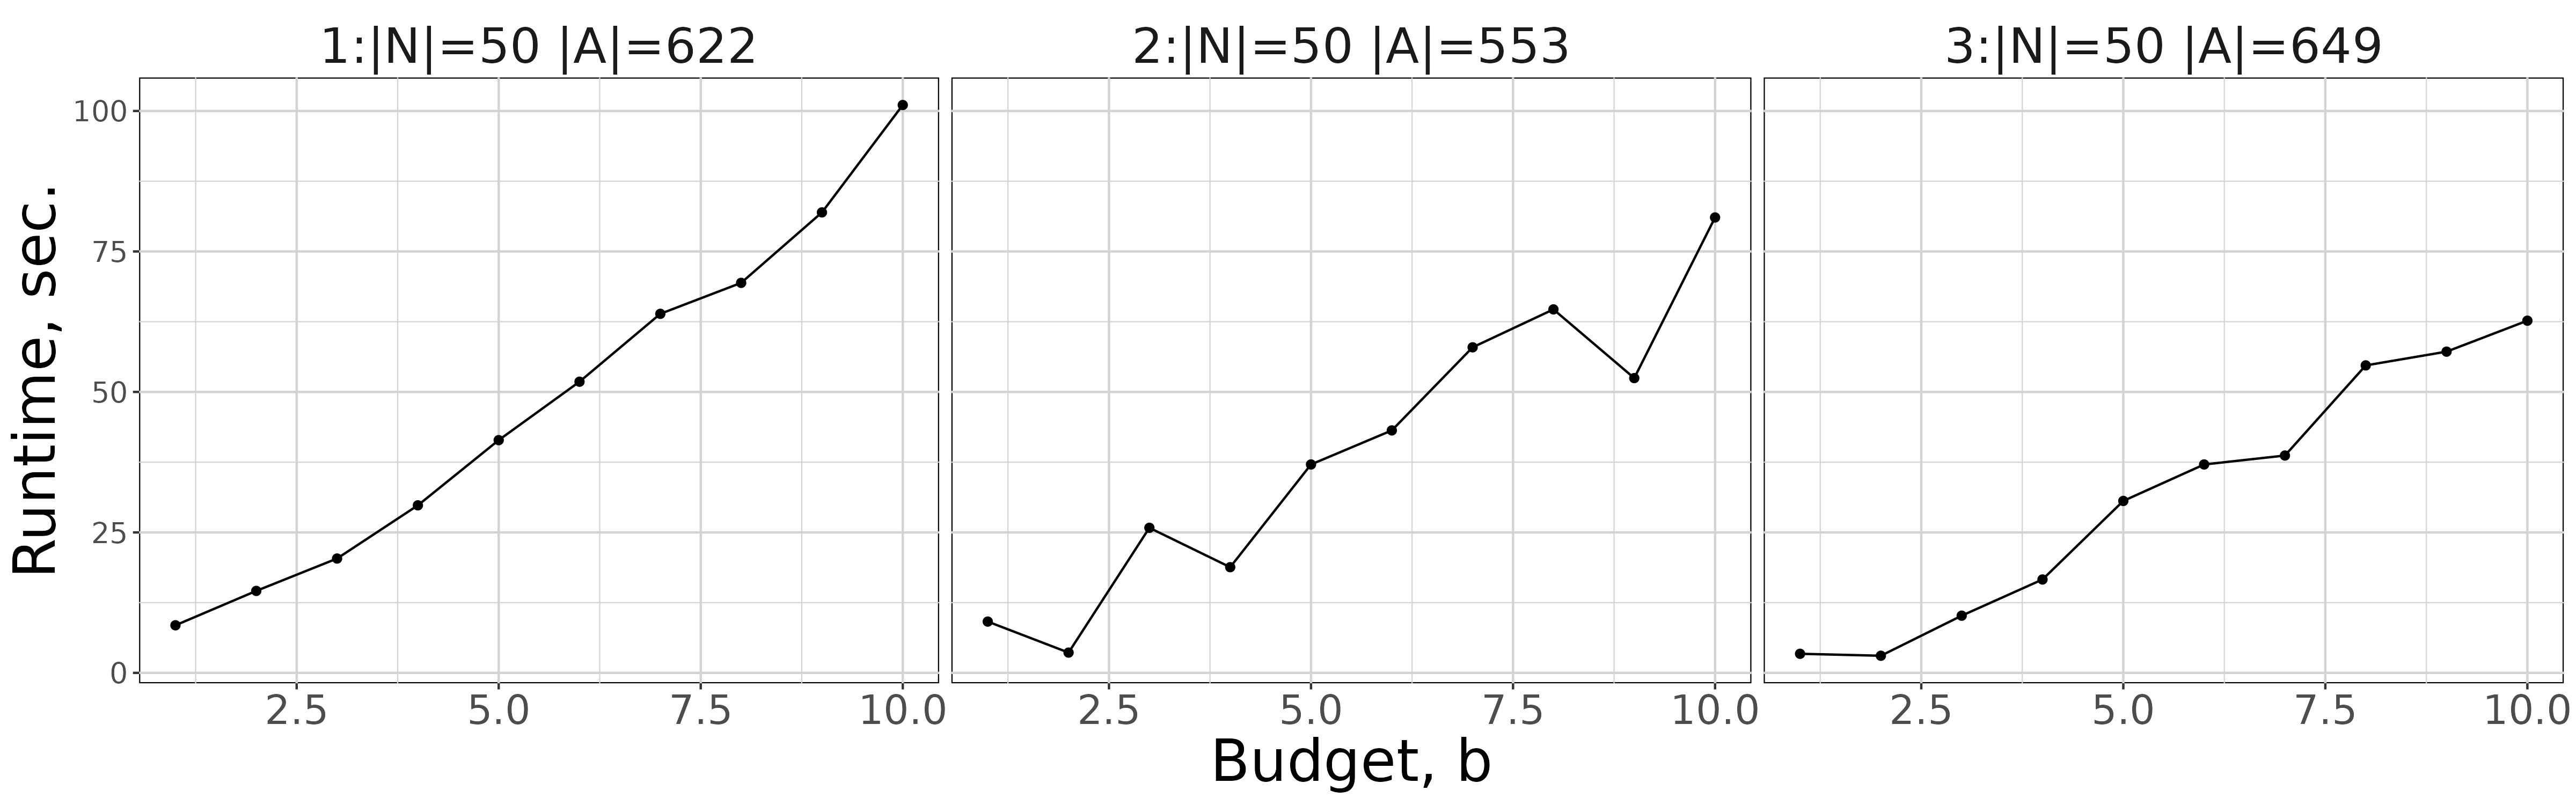
\includegraphics[width=\textwidth]{img/fig_runtimes.png}
\end{figure}
\end{frame}
\begin{frame}[label={sec:orgdc95029}]{Convergence profiles}
\begin{minipage}{0.45\textwidth}
{\scriptsize \centering $\varepsilon=0.05$\vspace{1ex} \\}
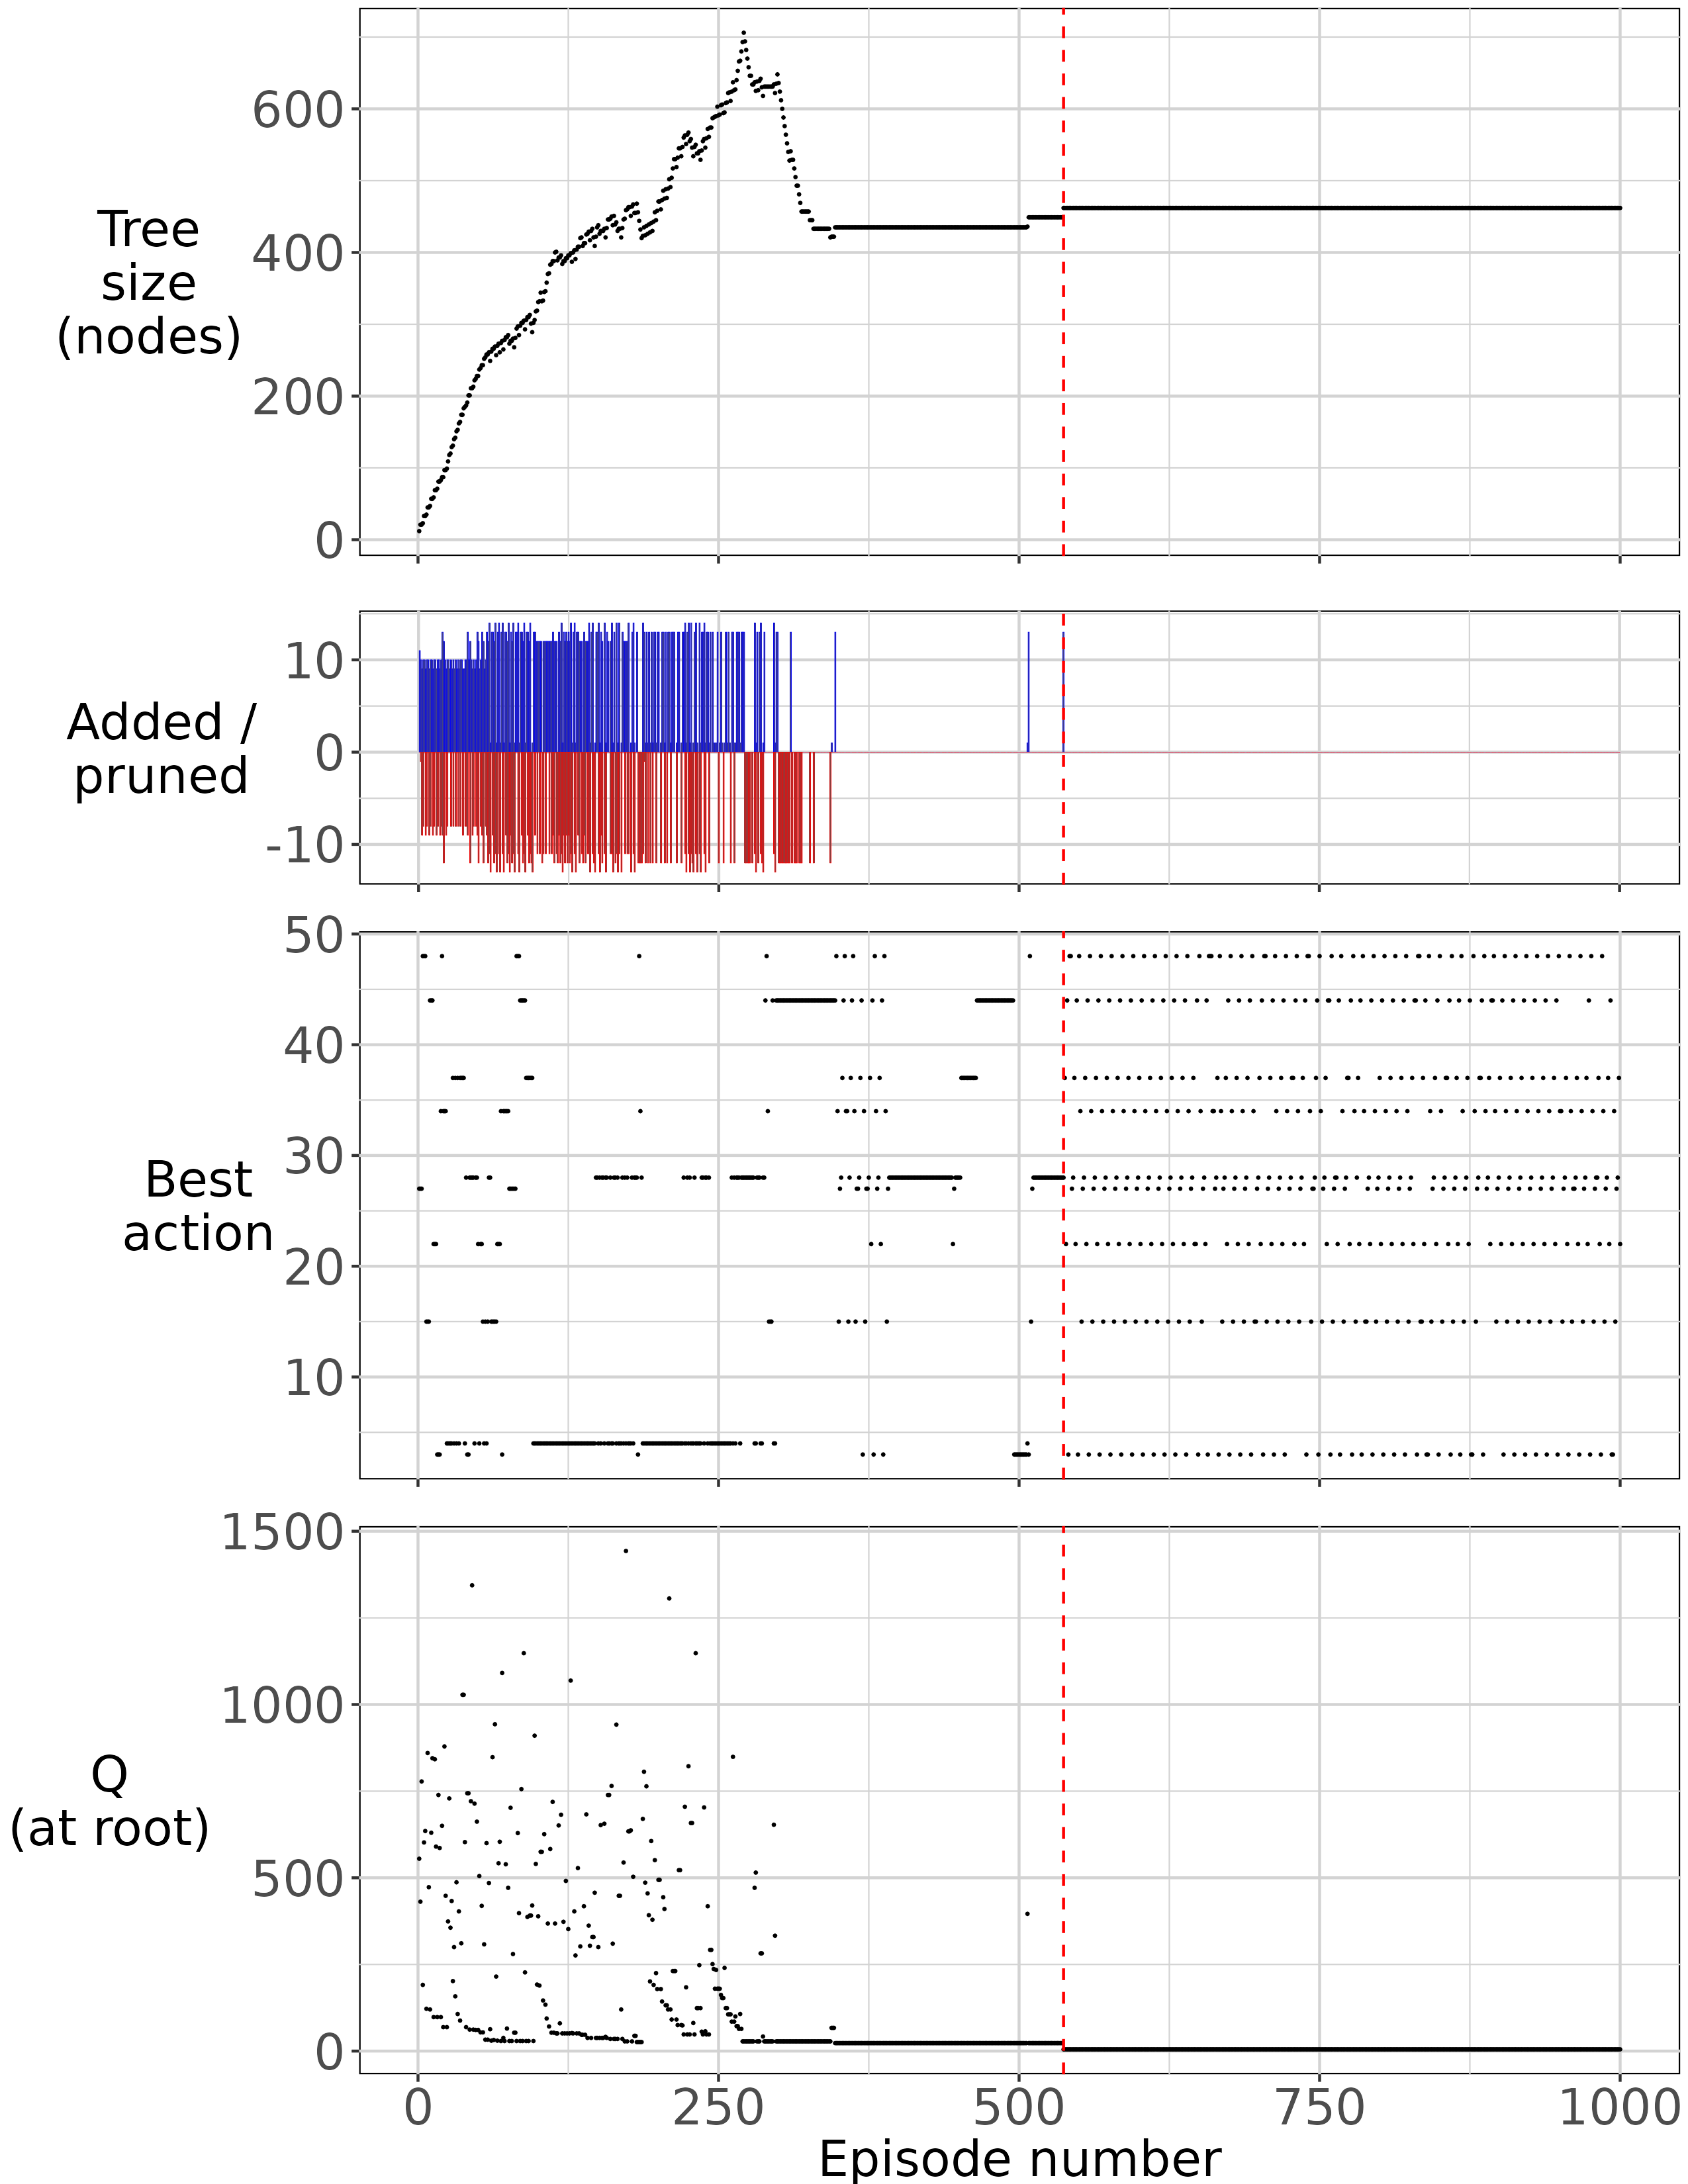
\includegraphics[width=0.4\paperwidth]{img/conv_profile_2eps_0.05.png}
\end{minipage}\hfill
\begin{minipage}{0.45\textwidth}
{\scriptsize \centering $\varepsilon=0.5$\vspace{1ex} \\}
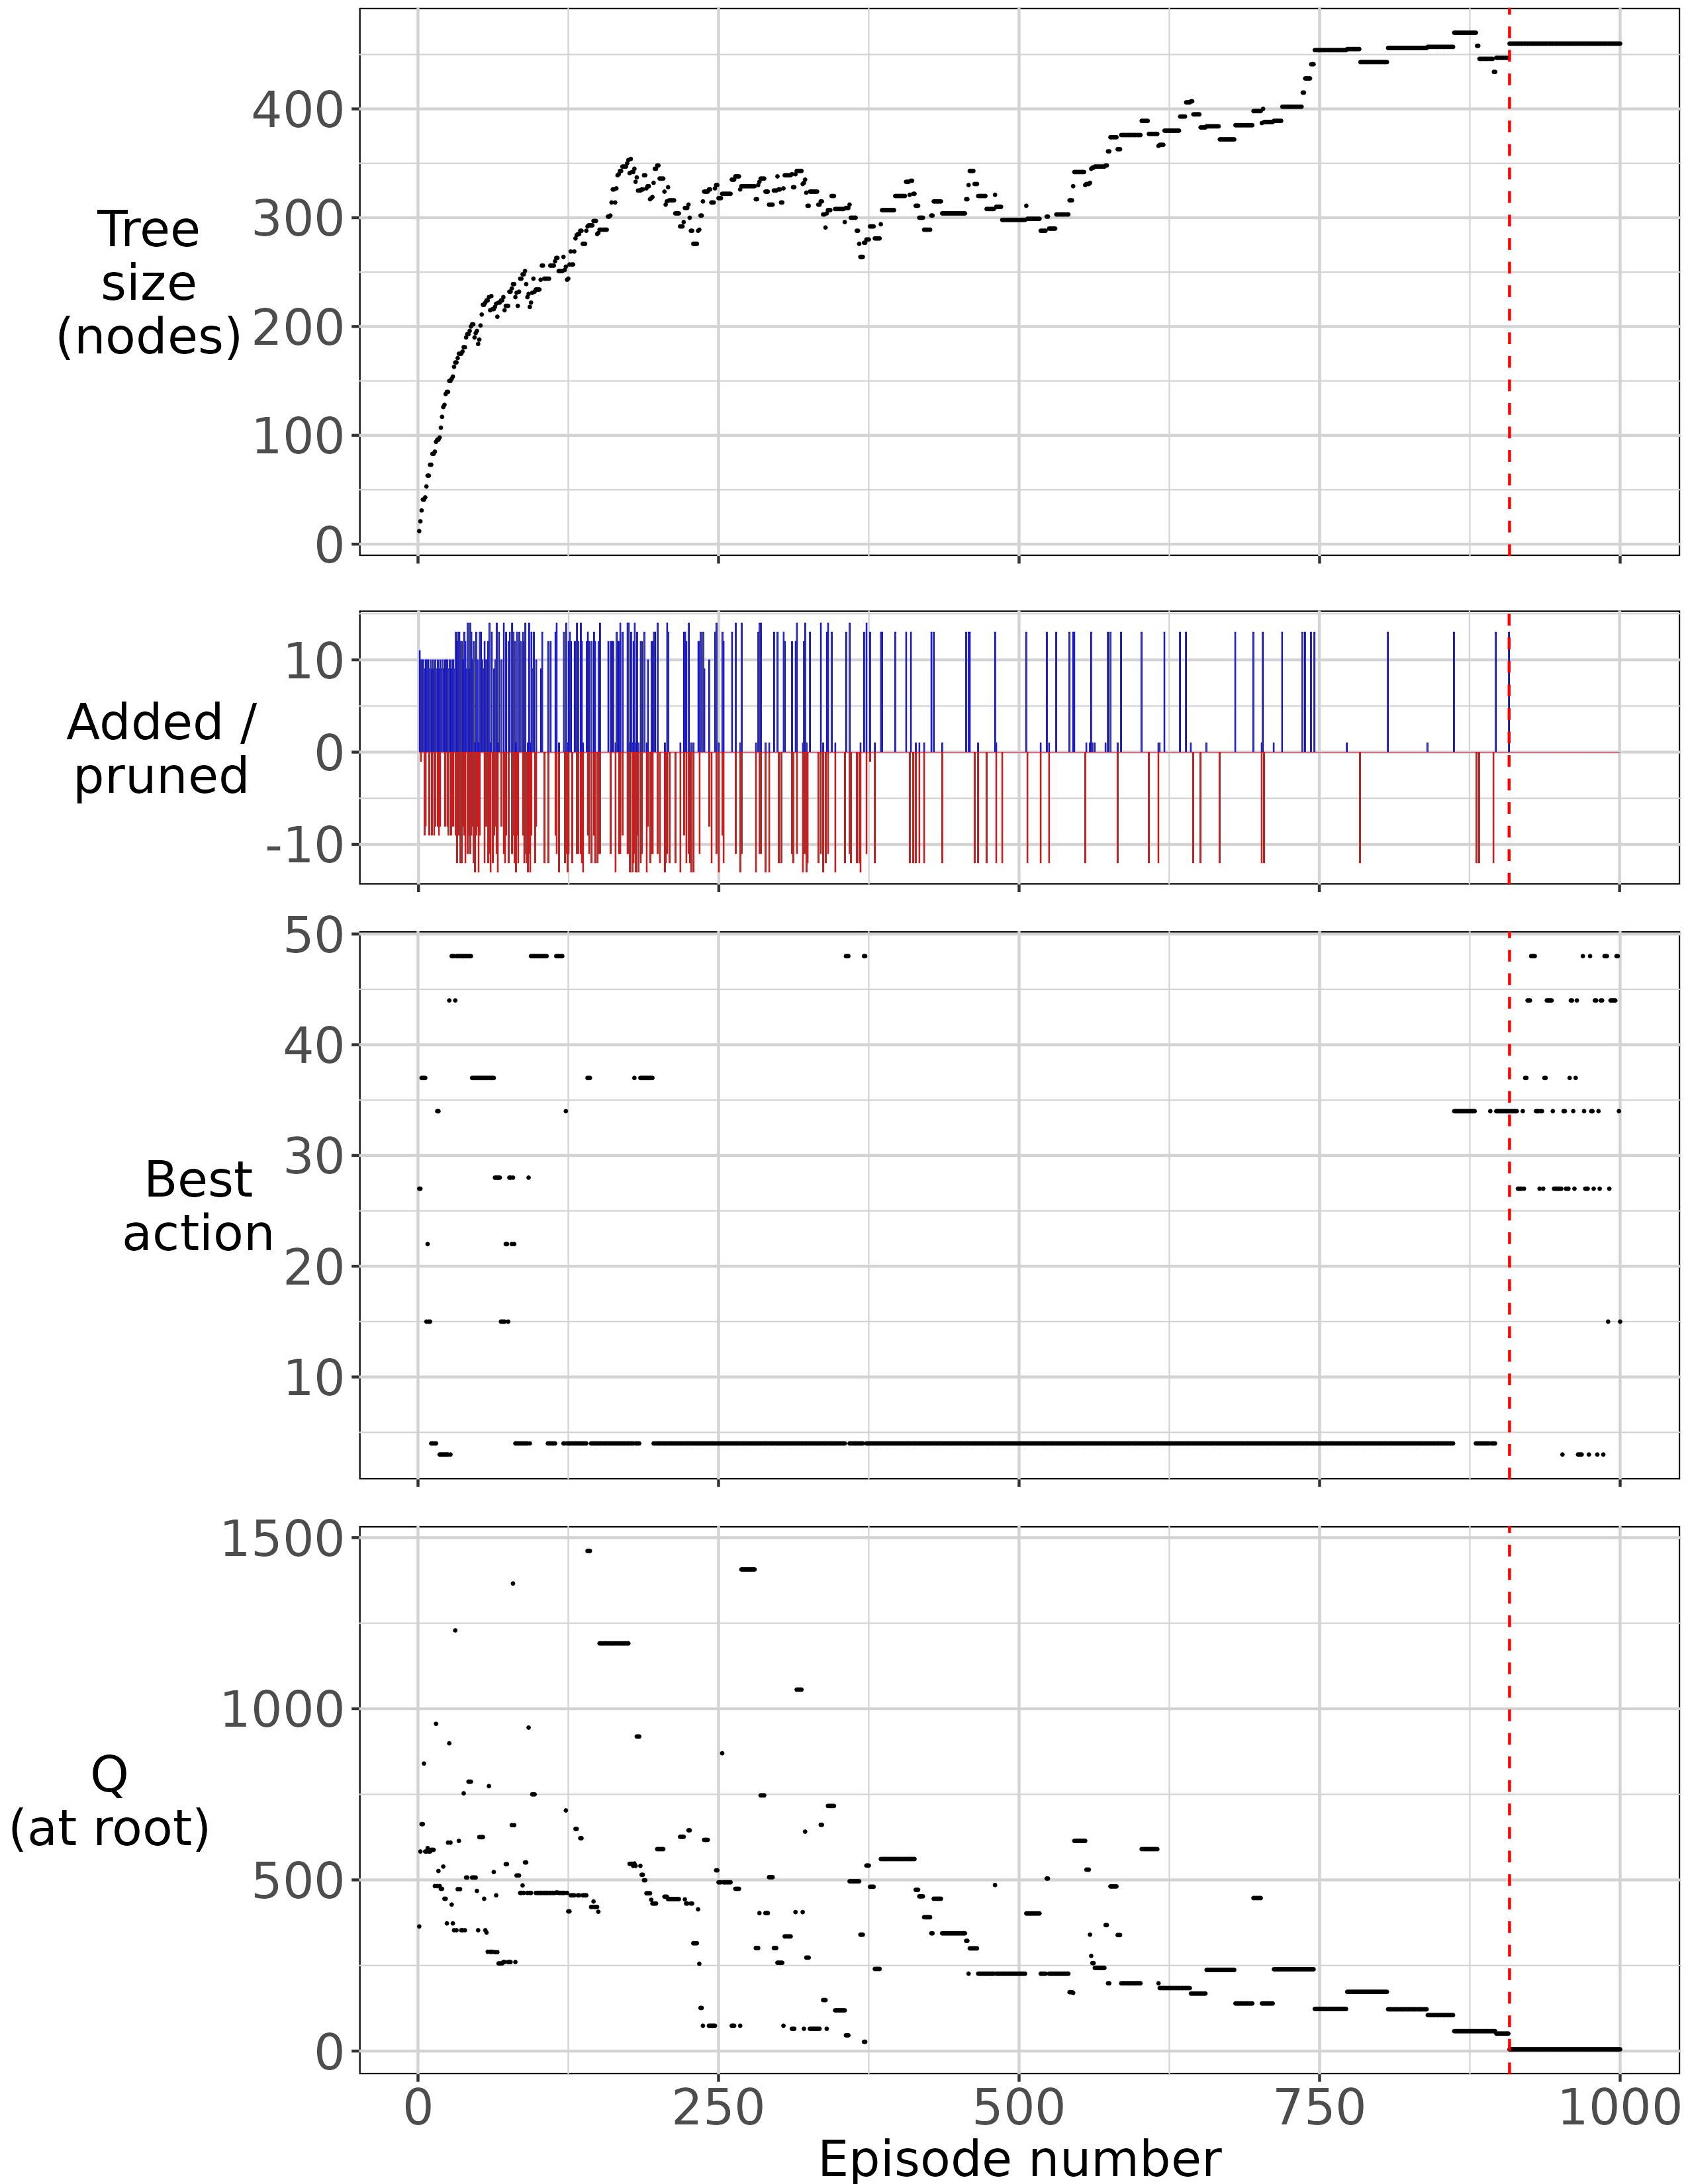
\includegraphics[width=0.4\paperwidth]{img/conv_profile_2eps_0.5.png}%
\end{minipage}
\end{frame}
\begin{frame}[label={sec:org647e23f}]{A remark: that's not just different runs}
\begin{columns}
\begin{column}{0.6\columnwidth}
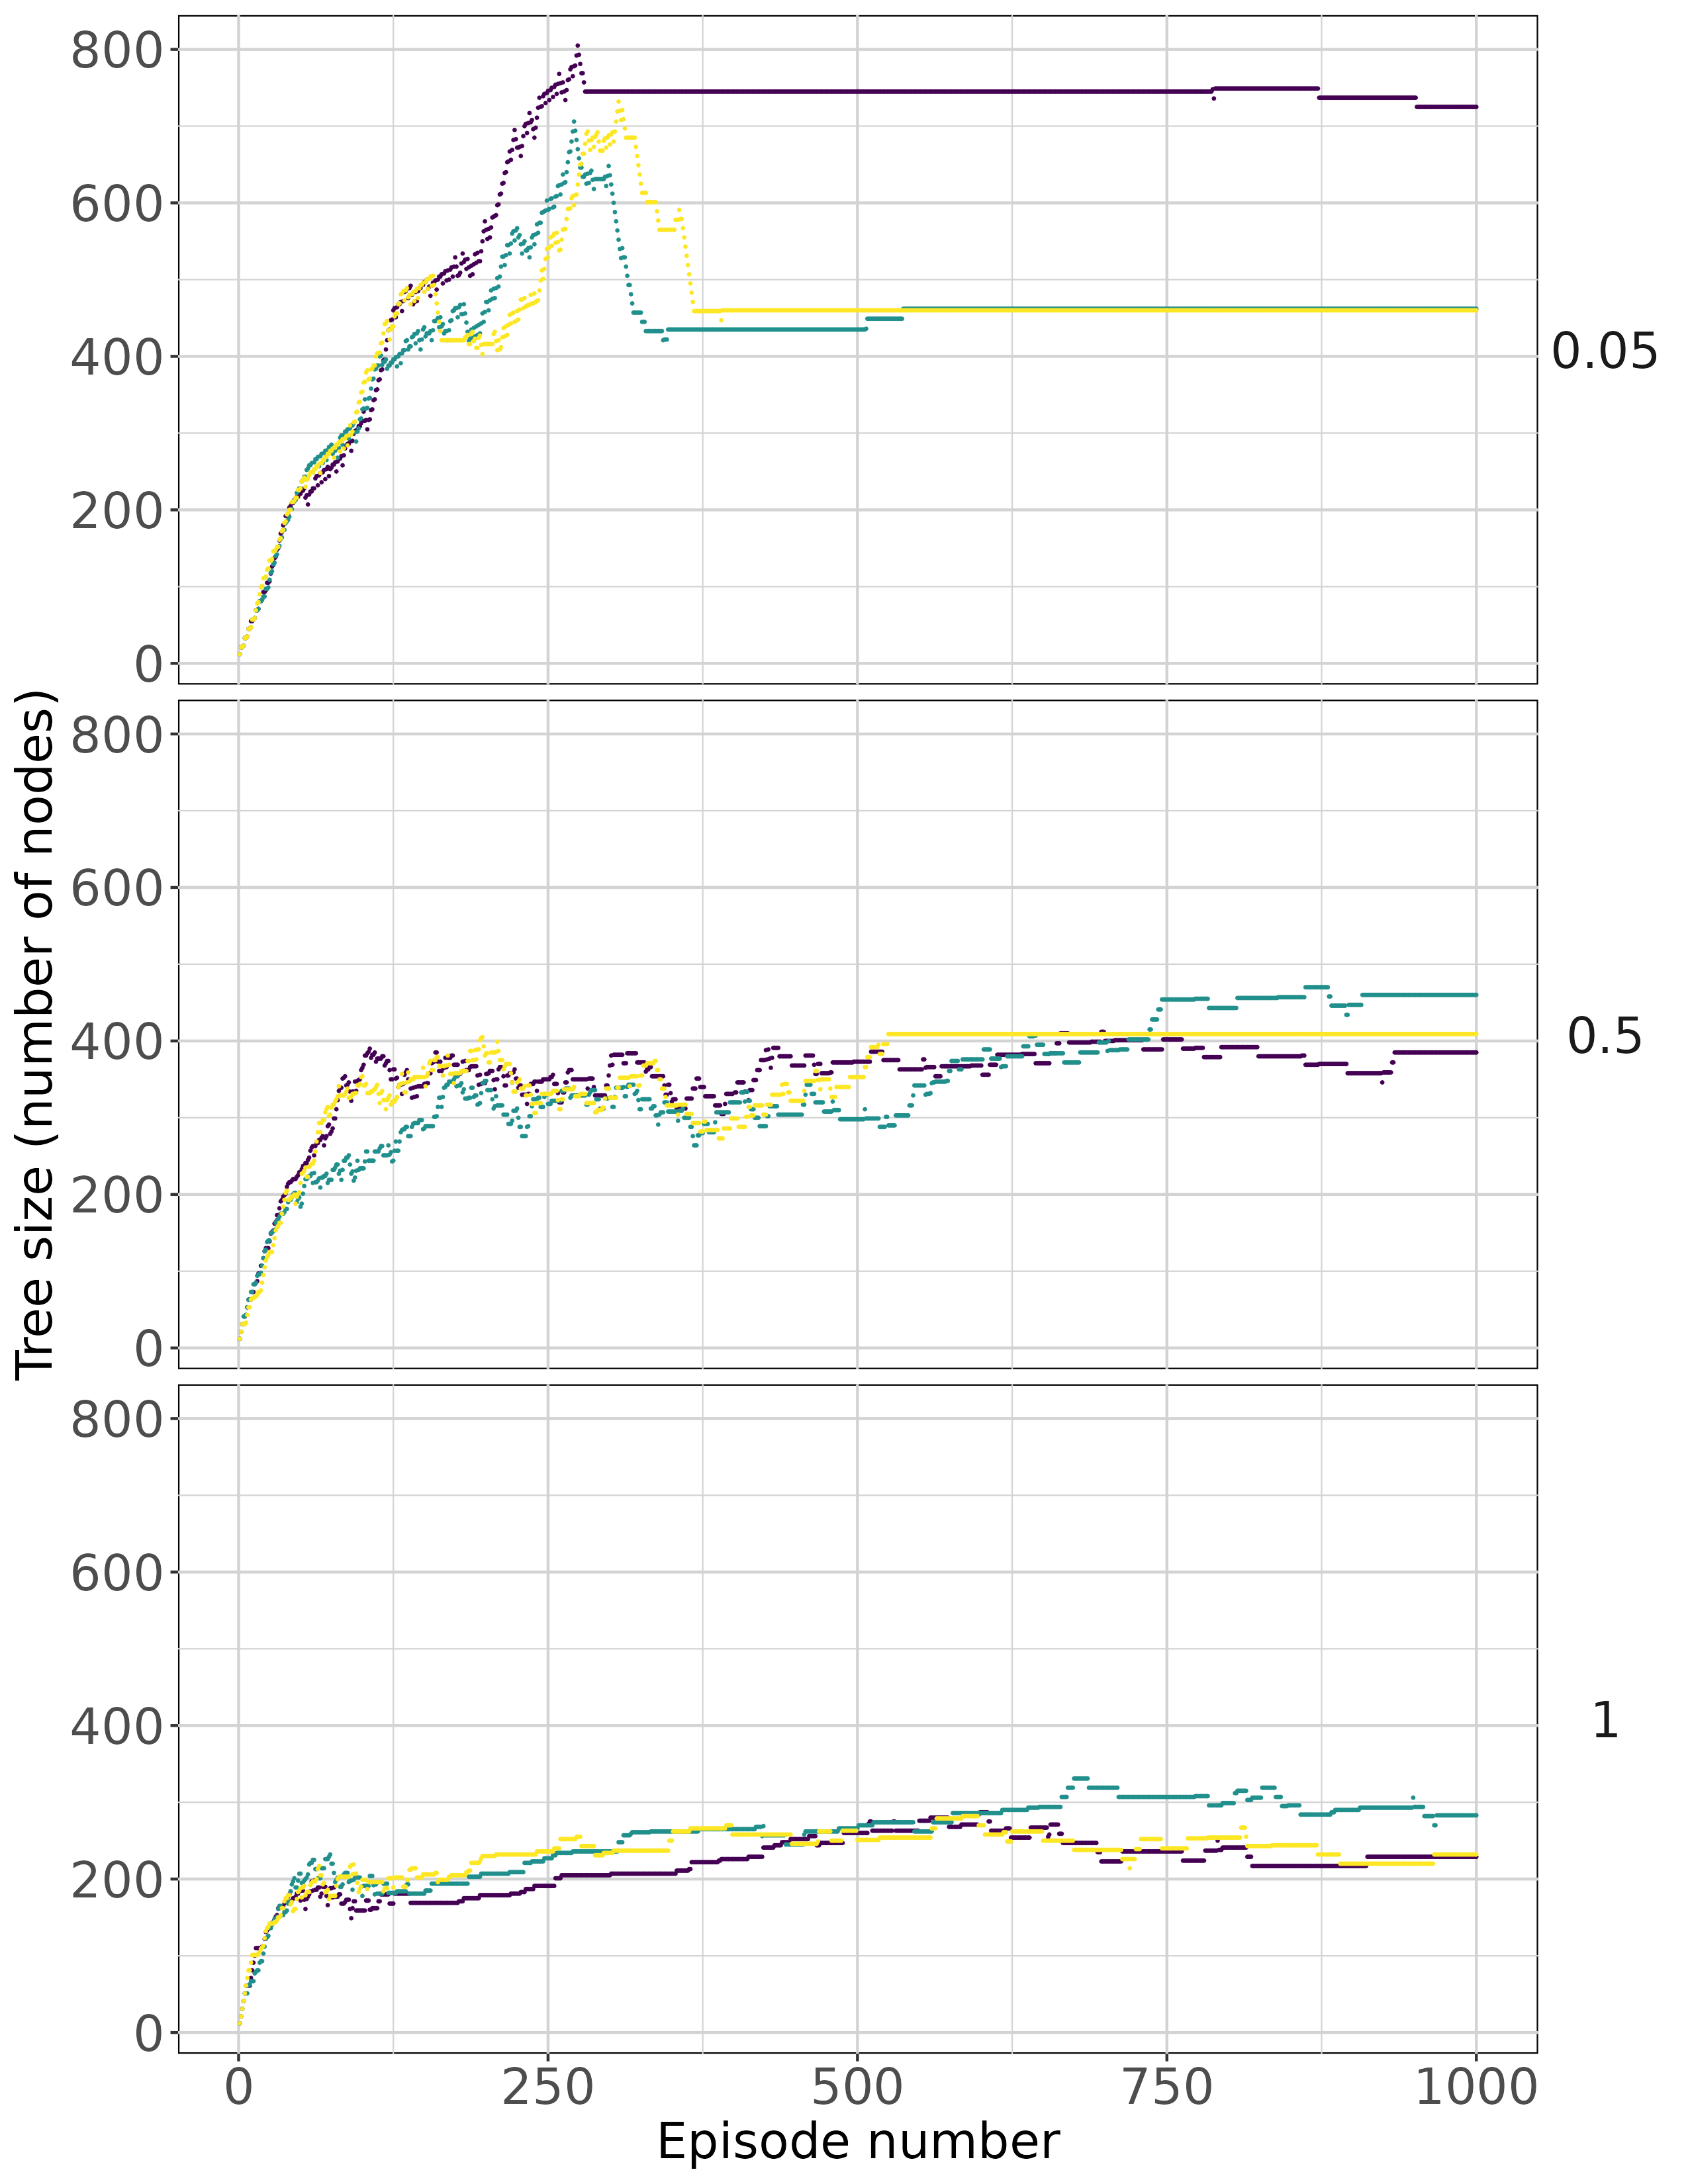
\includegraphics[height=0.8\textheight]{img/treesizes.png}
\end{column}
\begin{column}{0.4\columnwidth}
For each value of \(\varepsilon\) (0.05, 0.5, and 1) we performed three runs, to confirm these are indeed different ``modes'' of the algorithm.
\end{column}
\end{columns}
\end{frame}

\begin{frame}[label={sec:org03253ec}]{Play-out vs. first-move strategy}
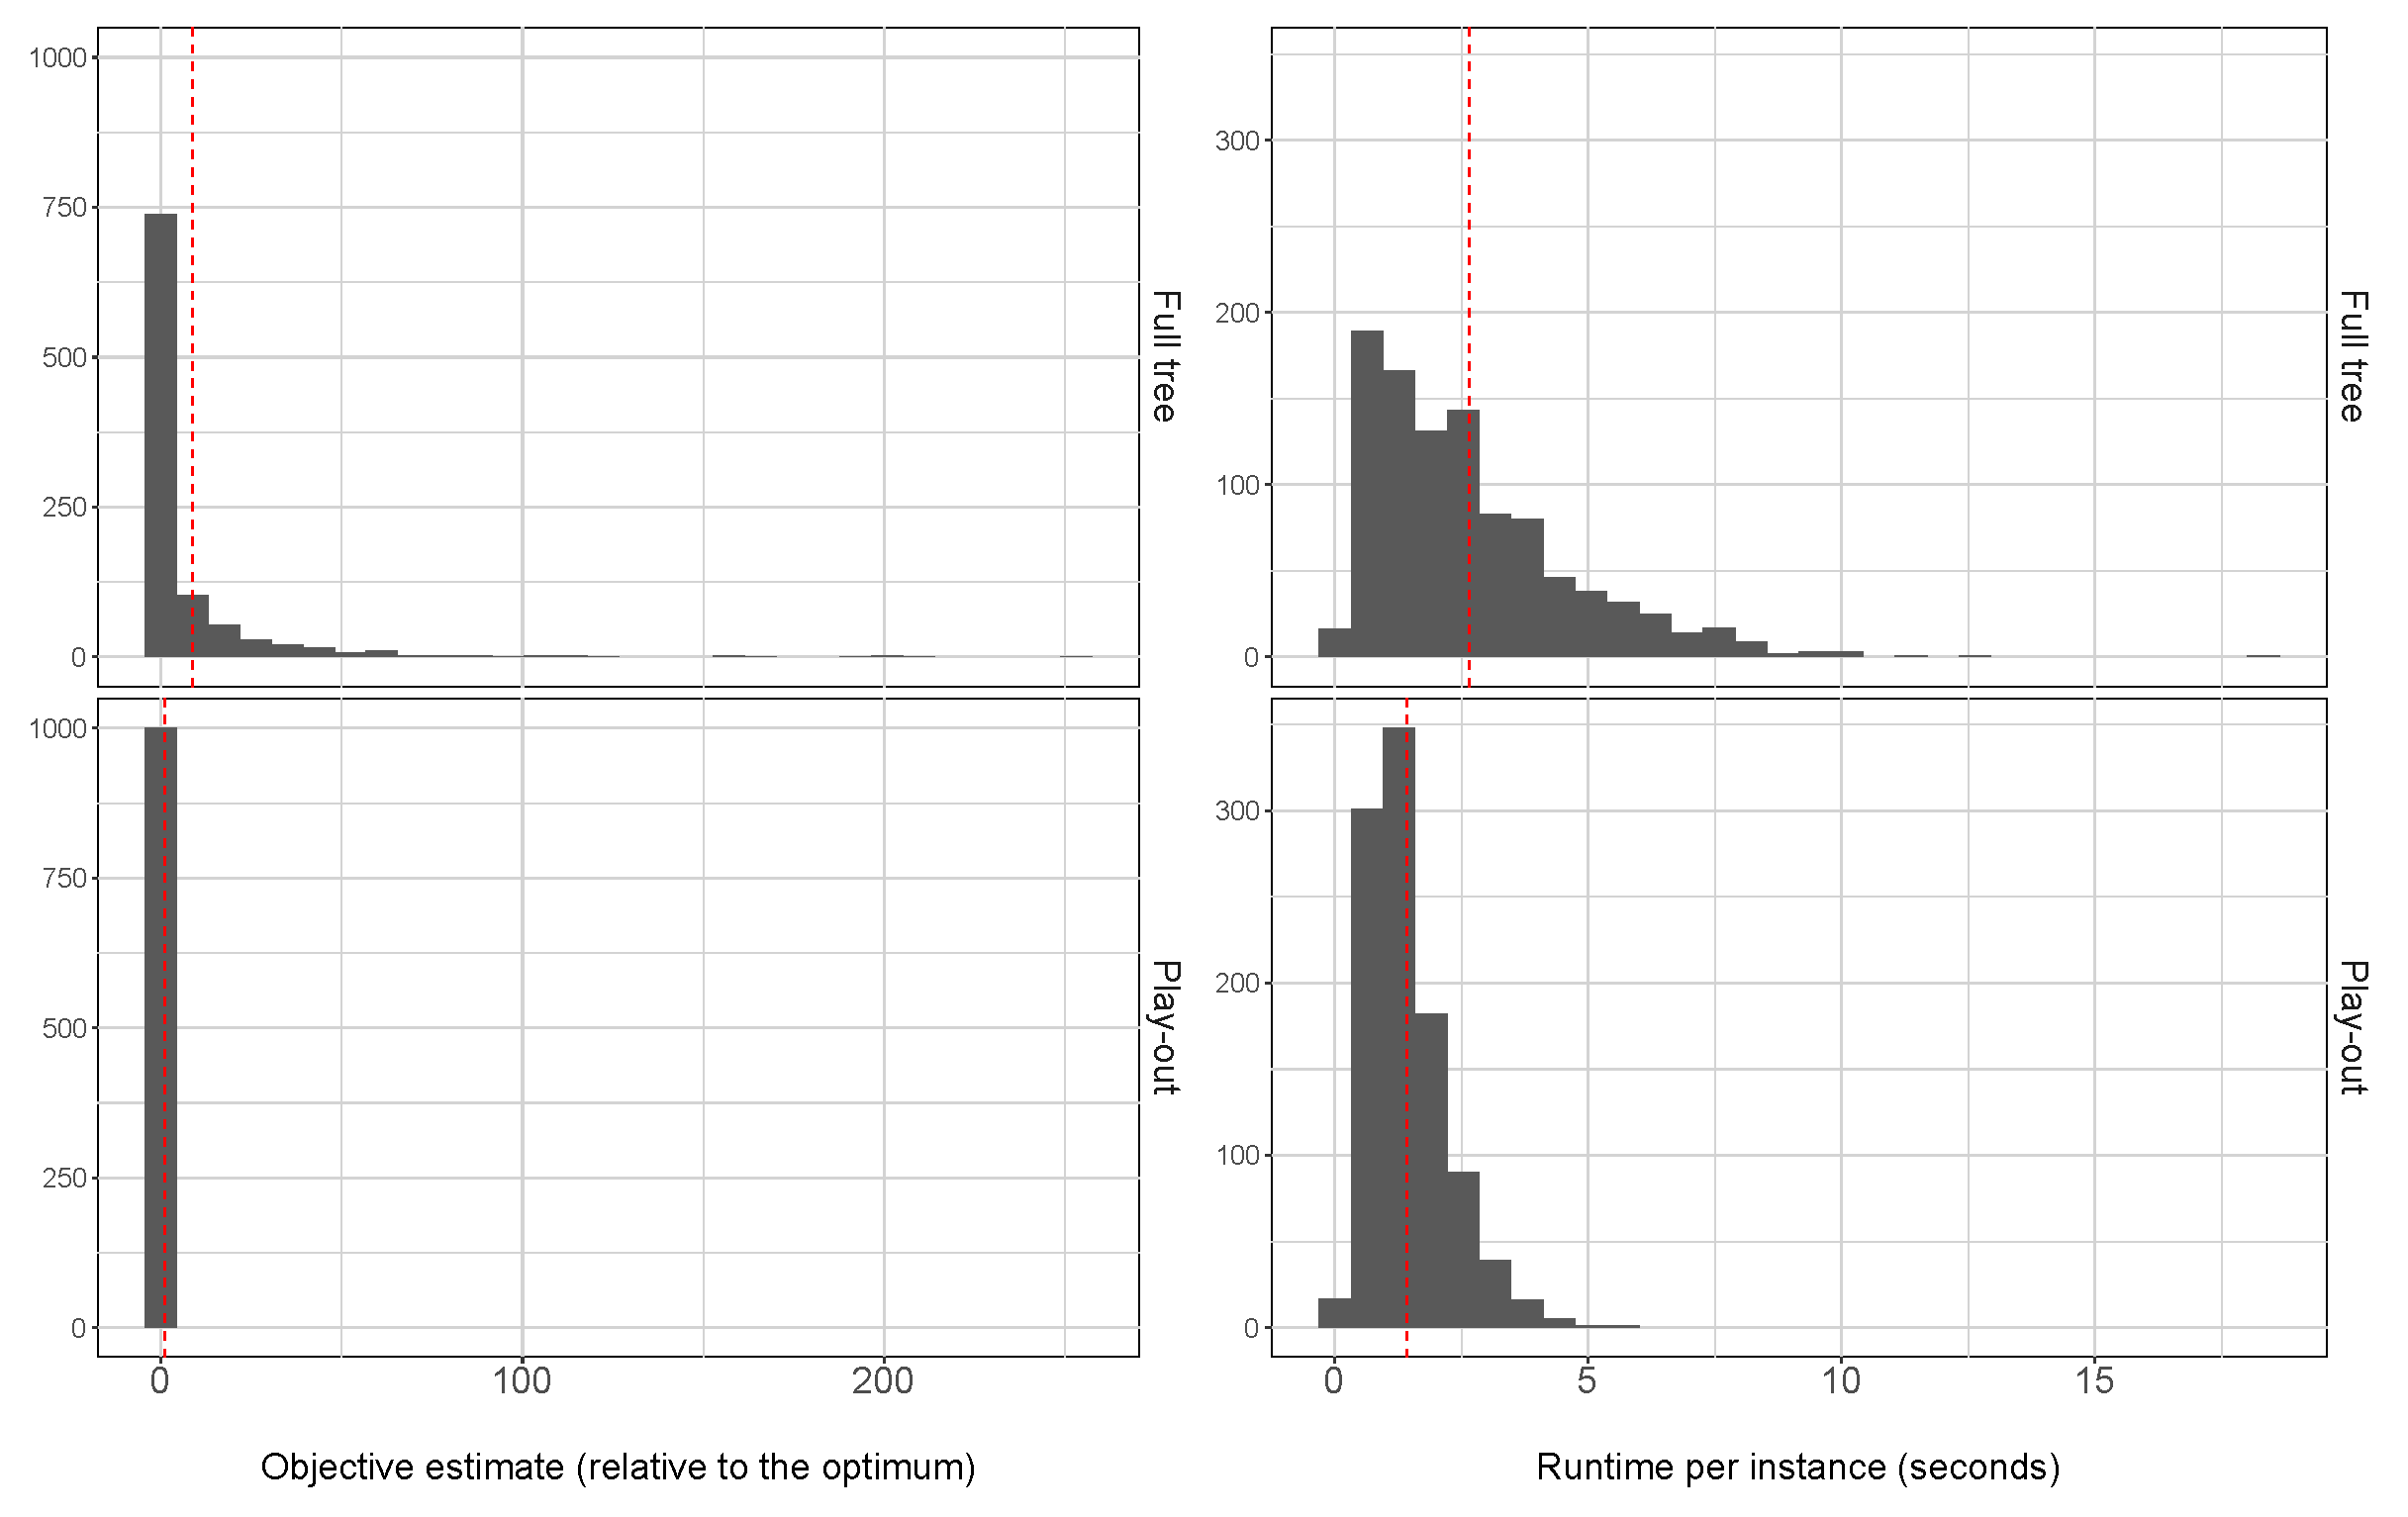
\includegraphics[width=\textwidth]{img/courage.eps}
\end{frame}
\subsection{On correctness}
\label{sec:org04b76b3}
\begin{frame}[label={sec:org9018422}]{Why does it work? (A sketch on ``correctness'')}
\begin{theorem}[Proposition]
$$\lim_{k\rightarrow \infty} \mathbb{P}\{Q^k_{\rnode{}} = \textrm{true optimum}\}=1$$
\end{theorem}
A sketch of the proof:

\begin{itemize}
\item The game tree has finite number of nodes (there is a bound independent from \(K\)).
\item We never cut off all the optima \(\Rightarrow\) the tree contains at least one.
\item What is left is a finite-size minimax tree, containing an optimum.
\item As \(K\rightarrow\infty\), probability to select every node for expansion converges to 1.
\end{itemize}
\end{frame}

\begin{frame}[label={sec:org1b5186c}]{Why in the world the tree is finite?}
\begin{columns}
\begin{column}{0.15\columnwidth}
Network:
\centering
\begin{tikzpicture}[%level distance=5mm,
  level 1/.style={level distance=10mm,sibling distance=12mm},
  level 2/.style={level distance=10mm,sibling distance=7mm},
  level 3/.style={level distance=10mm,sibling distance=7mm},
  font=\scriptsize,inner sep=2pt,
  every node/.style={draw=black, circle}]
  \node[draw=none] {...}
  child {node (a) {1}
    child {node (b) {2}
      child {node (c) {3}
        child {node[draw=none] {...}}
        child {node[draw=none] {...}}
        edge from parent node[left, draw=none] {$c_{23}$}}
      edge from parent node[left, draw=none] {$c_{12}$}}};
  \draw[->, bend right, shorten >=2pt, shorten <=2pt] (b.east) to (a.east);
  \node[draw=none, fill=none, xshift=7mm] at ($(a)!.5!(b)$){$c_{21}$}; 
\end{tikzpicture}\pause
\end{column}
\begin{column}{0.30\columnwidth}
After the \alert{first} expansion:
\vspace{2ex}

\centering
\begin{tikzpicture}[%level distance=5mm,
  level 1/.style={level distance=10mm,sibling distance=12mm},
  level 2/.style={level distance=10mm,sibling distance=7mm},
  level 3/.style={level distance=10mm,sibling distance=15mm},
  font=\scriptsize,inner sep=5pt,
  every node/.style={draw=black}]
  \node[draw=none] {...}
  child {node {$p=1$}
    child {node (A) {$p=2$}
      child {node (B) {$p=1$}}
      child {node (C) {$p=3$}}}};
  \node[draw=none, xshift=-3mm] at (A.west) {$(A)$};
  \node[draw=none, xshift=-3mm] at (B.west) {$(B)$};
  \node[draw=none, xshift=3mm] at (C.east) {$(C)$};
\end{tikzpicture}
\pause
\end{column}
\begin{column}{0.5\columnwidth}
After the \alert{second} expansion:
\vspace{2ex}

\centering
\begin{tikzpicture}[%level distance=5mm,
  level/.style={level distance=10mm,sibling distance=20mm},
  level 3/.style={sibling distance=30mm},
  font=\scriptsize,inner sep=5pt,
  every node/.style={draw=black}]
  \node[draw=none] {...}
  child {node {$p=1$}
    child {node (nA) {$p=2$}
      child {node[blue] (tn1) {$p=1$}
        child {node[blue] {$p=2$}
          child {node[blue] {$p=1$}
            child {node[draw=none] {...}}
            edge from parent[blue]}
          child {node[blue] (D) {$p=3$}
            child {node[draw=none] {...}}
            child {node[draw=none] {...}}
            edge from parent[blue]}
            edge from parent[blue]}
            edge from parent[blue]}
      child {node (nexit) {$p=3$}
        child {node[draw=none] {...}}
        child {node[draw=none] {...}}}}};
  \node[draw=none, xshift=3.5mm] at (nexit.east) {$(C)$};
  \node[draw=none, xshift=3.5mm] at (D.east) {$(D)$};
  \node[draw=none, xshift=-3mm] at (nA.west) {$(A)$};
  \node[draw=none, xshift=-3.5mm] at (tn1.west) {$(B)$};
\end{tikzpicture}
\end{column}
\end{columns}
\end{frame}
\section*{{\bfseries\sffamily TODO} Conclusion}
\label{sec:org4728b51}
\subsection*{Summary}
\label{sec:orgb0bc5c0}
\subsection*{Future research}
\label{sec:org6fa1ce6}

\begin{frame}[label={sec:orgf9f51bf}]{Mentioned sources}
 \scriptsize
\bibliographystyle{unsrtnat}
\bibliography{../../Dropbox/bibliography/references}
\end{frame}
\end{document}